\iffalse % CHANGE TO iffalse FOR RELEASE
\documentclass[letterpaper,10pt,oneside]{book}
\usepackage[compact]{titlesec}   % Reduce the space between titles and text
\titleclass{\chapter}{straight}
\titleformat{\chapter}[display]
  {\normalfont\huge\bfseries}{\chaptertitlename\ \thechapter}{20pt}{\Huge}
\titlespacing*{\chapter} {0pt}{50pt}{40pt}
\else
\documentclass[letterpaper,12pt]{book}
\usepackage{setspace}
\onehalfspacing
\fi


\usepackage{geo}
\renewcommand{\topic}[1]{#1}
\usletter

\usepackage[utf8]{inputenc}        % UTF code sequences in the input
\usepackage{times}                 % Times New font
\usepackage{pifont}                % Ding symbols (for Cloud9)
\usepackage{wasysym}               % For the bullets in the interpreter comparison (Chef)
\usepackage{multirow}              % Cells spanning rows in tables
\usepackage{xspace}
\usepackage[labelfont=bf]{caption} % Bold caption labels
\usepackage{wrapfig}               % Side figures without caption
\usepackage{framed}                % Framed paragraphs
\usepackage[linesnumbered,vlined]{algorithm2e} % Nice-looking algorithms
\SetAlgoCaptionSeparator{.}




%% Global definitions
\newcommand{\thesistitle}{Improving Scalability of Symbolic Execution for Software with Complex Environment Interfaces}

%\newcommand{\codebit}[1]{\textsf{\footnotesize #1}}
\newcommand{\codebit}[1]{\texttt{\footnotesize \bfseries #1}}

%% Cloud9 definitions
\newcommand{\cnine}{Cloud9\xspace}
\newcommand{\cninesuffix}{cloud9}

\newcommand{\cI}{\!{\raisebox{-0.2ex}{\large\ding{192}}}\xspace}
\newcommand{\cII}{\!{\raisebox{-0.2ex}{\large\ding{193}}}\xspace}
\newcommand{\cIII}{\!{\raisebox{-0.2ex}{\large\ding{194}}}\xspace}
\newcommand{\cIV}{\!{\raisebox{-0.2ex}{\large\ding{195}}}\xspace}
\newcommand{\cV}{\!{\raisebox{-0.2ex}{\large\ding{196}}}\xspace}
\newcommand{\cVI}{\!{\raisebox{-0.2ex}{\large\ding{197}}}\xspace}
\newcommand{\cVII}{\!{\raisebox{-0.2ex}{\large\ding{198}}}\xspace}
\newcommand{\cVIII}{\!{\raisebox{-0.2ex}{\large\ding{199}}}\xspace}

%% Chef definitions
\newcommand{\chef}{Chef\xspace}

\newcommand{\cmark}{\ding{51}}
\newcommand{\xmark}{\ding{55}}

\newcommand{\nicese}{NICE\xspace}
\newcommand{\cutiepy}{CutiePy\xspace}
\newcommand{\commuterse}{Commuter\xspace}


\usepackage{type1cm}
\usepackage{eso-pic}
% Use pdfsync in draft mode
%\usepackage{pdfsync}

\makeatletter
\AddToShipoutPicture{%
            \setlength{\@tempdimb}{.50\paperwidth}%
            \setlength{\@tempdimc}{.97\paperheight}%
            \setlength{\unitlength}{1pt}%
            \put(\strip@pt\@tempdimb,\strip@pt\@tempdimc){%
        \makebox(0,0){\textcolor[gray]{0.75}%
        {\fontsize{8mm}{8mm}\selectfont{DRAFT}}}}%
}
\AddToShipoutPicture{%
            \setlength{\@tempdimb}{.50\paperwidth}%
            \setlength{\@tempdimc}{.03\paperheight}%
            \setlength{\unitlength}{1pt}%
            \put(\strip@pt\@tempdimb,\strip@pt\@tempdimc){%
        \makebox(0,0){\textcolor[gray]{0.75}%
        {\fontsize{8mm}{8mm}\selectfont{DRAFT}}}}%
}
\makeatother



%% PDF SUPPORT
%% -----------

\usepackage[hidelinks]{hyperref} % Add cross references inside the PDF
\usepackage[all]{hypcap} % Fix the jump position when clicking figure references

\hypersetup{
  pdftitle={\thesistitle},
  pdfauthor={Stefan Bucur}
}

\begin{document}

\title{\thesistitle}
\author{Stefan Bucur \\ EPFL, Switzerland}

\maketitle

\chapter*{Abstract (German)}

Testen von Software ist aufwändig, zeitintensiv, und fehleranfällig. Symbolische Ausführung von Software ist eine vielversprechende Technik zum automatischen Erstellen von Testfällen. In der Praxis limitiert jedoch das Umgebungsproblem die Skalierbarkeit von symbolischer Ausführung: Software ist auf komplexe Schnittstellen zu ihrer Umgebung angewiesen, und die symbolische Ausführungsplattform sollte diese Schnittstellen bereitstellen. Es ist schwierig, das Umgebungsproblem ein für alle mal zu lösen, denn seine Natur hängt von der gegebenen Schnittstelle und ihrer Implementierung ab.

Diese Doktorarbeit behandelt zwei Fälle des Umgebungsproblems, welche zusammen ein breites Spektrum von praxisrelevanter Software abdecken: (1) Systemprogramme, welche mit dem Betriebssystem interagieren, und (2) Programme, welche in höheren, dynamischen Sprachen wie Python, Ruby oder JavaScript geschrieben sind. Diese beiden Fälle haben entgegengesetzte Eigenschaften: Betriebssystemschnittstellen sind typischerweise stabil und gut dokumentiert (z.B. POSIX); demgegenüber sind die Spezifikationen von dynamischen Sprachen partiell und unbeständig.

Um das Umgebungsproblem im Fall von stabilen Betriebssystemschnittstellen zu lösen, stellt diese Doktorarbeit \emph{\cnine} vor: eine Plattform zur symbolischen Ausführung mit einem genauen und effizienten Modell der POSIX Schnittstellen, wie sie von Systemprogrammen, Webservern und verteilten Systemen benutzt werden. \cnine beruht auf der Erkenntnis, dass die Betriebssystemschnittstelle zu Testzwecken durch ein Modell ersetzt werden kann, welches innerhalb der Testumgebung läuft und auf wenigen grundlegenden Abstraktionen aufbaut: Threads und Prozesse, Synchronisation und Adressräume mit gemeinsam genutztem Speicher. Diese Abstraktionen müssen als primitive Operationen von der symbolischen Ausführungsplattform bereitgestellt werden, während die restlichen Teile des Modells innerhalb der Testumgebung emuliert werden können.

Für den Fall der partiellen und unbeständigen Spezifikationen von dynamischen Sprachen stellt diese Arbeit \emph{\chef} vor. \chef erstellt symbolische Ausführungsplattformen für dynamische Sprachen, indem es deren Interpreter als ausführbare Spezifikation verwendet. \chef führt das zu testende Programm gemeinsam mit dem Interpreter auf maschinennaher Ebene (z.B. x86) symbolisch aus, so dass das Gesamtsystem zu einer symbolischen Ausführungsplattform auf höherer Ebene wird. \chef reduziert die Komplexität dieses Ansatzes mittels klassen-uniformer Pfadanalyse (class-uniform path analysis, CUPA), einer Heuristik zur Priorisierung von Pfaden. CUPA gruppiert Pfade in Äquivalenzklassen basierend auf Zielvorgaben der Analyse. 

\noindent \textbf{Keywords:} Symbolische Ausführung, Programmumgebungen, Systemsoftware, interpretierte Programmiersprachen.

\chapter*{Abstract}

Manual software testing is laborious, time-consuming, and subject to human error, yet it is the most common quality assurance method used in practice.
%
Automating the test case generation promises better effectiveness, especially for exposing corner-case bugs prone to oversight.
%
Symbolic execution is the most popular such technique to be applied on real-world software, as it has no false positives, it eventually enumerates all program executions, and can focus on parts of larger systems.
%
However, its scalability is limited by the \emph{environment problem}: to execute a program that relies on external functionality---its environment---the symbolic execution engine needs to efficiently support the environment interface.
%
Systematically addressing the environment problem is challenging, as its instances depend on the nature of the environment and its interface.

This thesis addresses two instances of the environment problem in symbolic execution, which collectively cover a wide range of real-world software: (1) system software interacting with the operating system, and (2) high-level programs written in dynamic languages, such as Python, Ruby, or JavaScript.
%
The two instances exhibit opposite characteristics: while the operating system interfaces are typically stable and well-documented (e.g., POSIX), the exact details of dynamic languages are left to implementations and continuously evolving.

To address the environment problem for stable operating system interfaces, this thesis introduces the idea of splitting an operating system model into a core set of primitives built into the engine, and the full operating system interface emulated on top in the guest.
%
As few as three primitives are sufficient to support a complex interface such as POSIX: threads and processes, synchronization, and address spaces with shared memory.
%
We prototyped this idea in \emph{\cnine}, a symbolic execution platform that provides an accurate and efficient model of the POSIX interface, as used by system such as utilities, web servers, and distributed systems.
%
\cnine is available at {\urlstyle{same}\url{http://cloud9.epfl.ch}}.

For programs written in dynamic languages, this thesis introduces the idea of using the language interpreter as an ``executable language specification''.  The interpreter runs inside a low-level (e.g., x86) symbolic execution engine, while it executes the target program.  The aggregate system acts as a language-level symbolic execution engine for the program.
%
To circumvent the complexity of symbolically executing the entire interpreter, this thesis introduces Class-Uniform Path Analysis (CUPA), a heuristic for prioritizing paths that works by grouping paths into equivalence classes according to a coverage goal.
%
We prototyped this idea in the \emph{\chef} symbolic execution platform for interpreted languages, available at {\urlstyle{same}\url{http://dslab.epfl.ch/proj/chef/}}.

\noindent \textbf{Keywords:} Symbolic execution, program environments, systems software, interpreted languages.


%%% Local Variables: 
%%% mode: latex
%%% eval: (visual-line-mode)
%%% fill-column: 1000000
%%% TeX-master: "main"
%%% End:



\chapter*{Acknowledgments}
This work would not have happened without the people who have supported me throughout this journey.


I~am deeply grateful to my advisor, George Candea, an exceptional model of strength, vision, and kindness.
%
I~am indebted for his patience and wisdom, for pushing me out my comfort zone to become independent in pursuing my goals and reaching for the stars.  I feel very fortunate to having worked with him and I wouldn't have gotten this far without his mentorship.


I~thank my patient thesis committee: Vikram Adve, Johannes Kinder, Willy Zwaenepoel, and Jim Larus.  Their insightful comments and advice helped crystallize the vision of the thesis.


All the work presented here is the result of collaboration with many incredibly bright people.
%
I~am grateful to Johannes Kinder for his tenacious help with Chef.  During our many insightful discussions, he would bring clarity to the most difficult problems.
%
I~thank Vitaly Chipounov for helping me navigate the fine mechanics of the S2E system.
%
I~am indebted to Vlad Ureche, who was instrumental in Cloud9's successful encounter with real-world software.
%
I~thank Cristian Zamfir for his advice and patience during the most critical parts of my PhD.
%
I~thank Volodymyr Kuznetsov for his insights and for being a model of resourcefulness.
%
I~thank Martin Weber for his work and for giving me the chance to practice my mentoring. 
%
I~am grateful to Liviu Ciortea for easing my way to symbolic execution.
%
I~thank Istvan Haller, Calin Iorgulescu, Ayrat Khalimov, and Tudor Cazangiu for their contributions to Cloud9.


My PhD experience was defined by the interactions I had with the outstanding team in the Dependable Systems lab.
%
I~am truly grateful to Silviu Andrica, Radu Banabic, Vitaly Chipounov, Alex Copot, Horatiu Jula, Baris Kasikci, Johannes Kinder, Volodymyr Kuznetsov, Georg Schmid, Ana Sima, Jonas Wagner, Cristian Zamfir, and Peter Zankov for the inspiring moments and making the lab a fun place to be.
%
I~am especially thankful to Nicoletta Isaac, who made sure everything in the lab ran smoothly.


I~thank Ed Bugnion and Jim Larus for their inspiring advice and immensely useful lessons.
%
I~am thankful to Burak Emir and Lorenzo Martignoni, my mentors at Google, for their guidance and support.


I~thank Jonas Wagner for his precious help with translating the thesis abstract to German.
%
I~am sending special thanks to Amer Chamseddine, Lo\"{\i}c Gardiol, Benjamin Schubert, and Martin Weber for their valuable feedback on my presentation dry-runs and their availability on a short notice.


I~am grateful to Cristian Cadar, Daniel Dunbar, and Dawson Engler for creating and open-sourcing KLEE.  Beside serving as a foundation for my own work, I learned a lot about symbolic execution by studying and tinkering with its code.


I~thank Google for generously supporting a significant part of my research through a fellowship.
%
I~thank EPFL for providing me a unique working environment and unparallelled resources to pursue my work.
%
I~thank ERC for their important financial support.


I~thank my parents, Jana and Mihai Bucur, for their selfless support and encouragement to follow my dreams.  Any of my accomplishments bears the mark of their upbringing.
%
I~thank my brother, Andrei Bucur, for his care and inspiration.


I~thank Alexandra Olteanu for her tireless support and care, for her wisdom, and for being a pillar of strength throughout the years.

%%% Local Variables: 
%%% mode: latex
%%% eval: (visual-line-mode)
%%% fill-column: 1000000
%%% TeX-master: "main"
%%% End:


\tableofcontents
\listoffigures
\listoftables

\chapter{Introduction}
\label{ch:introduction}
In this chapter, we describe the problem being addressed in this thesis and present a brief overview of the solution we propose.
%
Subsequently, in Chapter~\ref{ch:relatedwork}, we describe in more depth the prior art and the work related to ours, to gain an understanding of the landscape in which our solution appeared.
%
The rest of the thesis covers our solution.

\section{Problem Definition}
\subsection{Limitations of Manual Software Testing}

A crucial aspect of software development is ensuring that the written code behaves as intended.  Today, this is particularly important, as software is playing an increasingly dominant role in our lives, from keeping our private data in the cloud to powering our ubiquitous smartphones.

Ideally, software would be written correctly by construction.  This was the way software engineering was envisioned in the early days of computer science~\cite{dijkstra1976discipline}; the code would be written together with the mathematical proof of its correctness.

However, the decades of software development experience that followed have painted a different picture.  As it turns out, the software complexity---up to hundreds of millions of lines of code---and rapid pace of feature development have precluded a formal, rigorous approach.
%
With the exception of a few safety-critical segments, such as avionics~\cite{Astree}, automotive~\cite{automotive}, or medical equipment, most of the software industry today relies on \emph{testing} for its quality assurance~\cite{softwareMetrics}.
%% %
%% In this thesis, we refer to such software as \emph{real-world software}, which we define more precisely as follows.

%% \medskip

%% \textbf{Definition:} We define \emph{real-world software} to be commodity software developed in industry in the form of products (e.g., browsers or CAD tools), services (e.g., web search or web-based email), building blocks (e.g., libraries), and developer support tools (compilers, benchmarks, etc.).
%% %
%% The development of real-world software is primarily governed by market and logistic constraints, such as budgets, shipping deadlines, and competition on features.
%% %
%% In this respect, real-world software distinguishes itself from safety-critical software developed in the automotive, avionics, or space industry.

%% \medskip

Testing a program consists of exercising multiple different paths through it and checking whether ``they do the right thing.''
%
In other words, testing is a way to produce partial evidence of correctness, and thus increase confidence in the tested software.
%
Yet, test suites provide inadequate coverage of all the inputs a program could handle.
%% Yet, due to the typically poor coverage one can get today, testing often turns into a mere hunt for bugs.
%
For instance, the test suite of the Chromium browser contains about one hundred thousands tests~\cite{chrome-tests}.  This suite is thoroughly comprehensive by industry standards, yet it represents only a small fraction of all possible inputs the browser may receive.

%% In practice, most software test harnesses consist of manually written tests that are run periodically; regression test suites provide an automated way of checking whether new bugs have entered the code~\cite{codeComplete}.
%
Test suites also tend to be tedious to write and maintain.  Statistics show that, on average, developers spend as much as half of their time doing testing~\cite{codeComplete}, and companies allocate up to a quarter of their IT budget for software testing~\cite{capgemini-world-quality}.

The net result is that, despite the effort and resources invested in manual testing, bugs escape quality assurance and make it into production~\cite{redHatSecurityX}.
%
The industry average for bug density is a staggering 15 errors per 1000 lines of shipped code, while the most thorough quality assurance processes reach 0.1 errors per 1000 lines of code~\cite{codeComplete}.

Today, this problem is amplified by having an increasing number of businesses online and hence vulnerable to remote attacks that exploit software vulnerabilities.  For instance, in 2014, there were 19 CVE vulnerabilities reported on average \emph{per day}~\cite{nvd}.
%
These vulnerabilities are exploited to cause major disruptions~\cite{sony-hack} or leaks of sensitive data~\cite{sony-hack,psp-hack}.  On average, a data breach cost \$3.8 million in 2015~\cite{breach2015}, and the most prominent cases cost over \$100 million~\cite{target-hack}.

%% Software testing is resource-hungry, time-consuming, labor-intensive, and prone to human omission and error.  A lot of bugs escape quality assurance into production, where they cause disruptions and data loss. For instance, in 2014, there were 19 CVE vulnerabilities reported on average per day, and estimates show that software bugs cost the global economy more than \$300 billion in 2013.

%% At the same time, resources invested in testing are peaking. In 2014, about a quarter of the entire IT budget in enterprises was allocated to software testing, which was the highest figure to that date.  On average, developer teams spend as much as half of their time doing testing and fixing bugs.

%% Facing this situation, organizations recognize that software testing is cumbersome.  In a recent survey, more than two thirds of the organizations questioned admitted they have difficulties determining relevant tests for their software and pointed at the lack of adequate tools to support that.

Alas, with a few exceptions---e.g., seL4~\cite{seL4}, a recent effort of formally verifying an operating system kernel---switching to a formal development model is not feasible for most of the software written today.
%
Despite recent advancements in formal techniques and tools, which have brought down the cost of building formally-proven software, it still takes on the order of person-years to develop a few thousand lines of verified code~\cite{seL4}.
%
This rate is currently unsustainable for most commodity software.
%
Therefore, the second best option today is to automate the software testing process itself.


\subsection{Automated Testing: Black-box vs. White-box}

The simplest (and most popular) form of automated testing consists of randomly generating program inputs and observing whether the program crashes~\cite{fuzz,quickcheck,afl,autodafe,skipfish}.
%
The inputs are typically obtained by fuzzing~\cite{fuzz}, i.e., randomly mutating a known valid input, such as an image file or a productivity suite document.  This form of testing is called ``blackbox'', because the input generation does not take into account the structure of the program under test~\cite{blackbox-testing}.
%
Despite their conceptual simplicity, fuzzers are effective at discovering  bugs~\cite{afl,autodafe,skipfish} (albeit shallow) and are currently the state of the practice in automated testing.

\begin{figure}
  \centering
  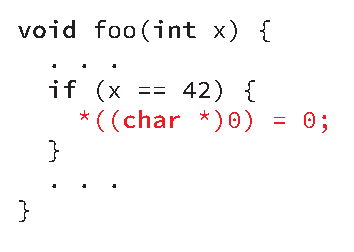
\includegraphics[width=2.0in]{introduction/figures/fuzzing-example}
  \caption{Example program for which random fuzzing is unlikely to uncover the memory error bug (the red line).}
  \label{fig:intro:fuzzing}
\end{figure}

However, plain random fuzzers are ineffective at discovering corner-case bugs---bugs that manifest only under particular inputs in the program.
%
Consider the simple example in Figure~\ref{fig:intro:fuzzing}, where the program checks the input for the particular value 42 before performing a null-pointer access.  A random fuzzer has \emph{less than one in a billion} chance of hitting the bug with each input generated.
%
The vast majority of the generated inputs are therefore redundant.

A better approach is ``greybox'' testing, i.e., to generate tests that follow a certain structure, as defined by a specification, such as protocol format~\cite{sulley}, grammar~\cite{quickcheck}, or input precondition~\cite{boyapati:korat}.
%
However, this method would still likely miss bugs whose triggering inputs are not exposed in the input specification.

The most precise approach is to take the program structure itself into account when generating inputs.
%
This form of testing is called ``whitebox''; its goal is to generate inputs that take the program along previously unexplored execution paths.
%
Symbolic execution is the most successful automated whitebox testing technique to be applied to commodity software, in terms of size of software and bugs found~\cite{sage2012,all-symbex,decades-symbex,practice-symbex}.

\subsection{Systematic Path Exploration Using Symbolic Execution}
\label{sec:intro:symbex}

\begin{figure}
  \centering
  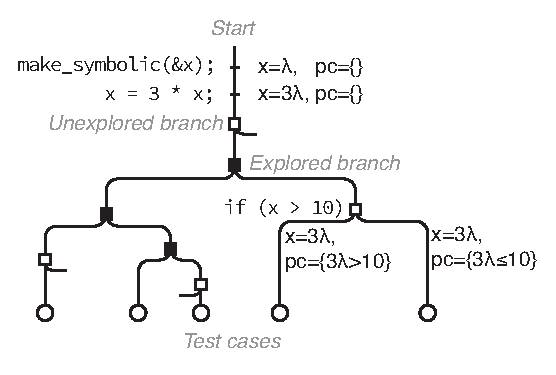
\includegraphics[width=3.5in]{introduction/figures/symbex-tree}
  \caption{Symbolic execution tree for a simple example.  Program states maintain symbolic values for variable \codebit{x} and carry a path condition (pc).}
  \label{fig:intro:symbex-tree}
\end{figure}

Symbolic execution works by executing a program with \emph{symbolic} instead of concrete input values, to cover the entire input space and thus all possible program execution paths (Figure~\ref{fig:intro:symbex-tree}).  For instance, a function \codebit{foo(int x)} is executed with a symbolic variable $\lambda$ assigned to \codebit{x}.
%
Statements using \codebit{x} manipulate it symbolically: \codebit{x := x * 3} updates the value of \codebit{x} to $3 \cdot \lambda$.  During execution, the assignment of variables to expressions is kept in a \emph{symbolic store} of the program execution state.

Whenever the symbolic execution engine encounters a conditional branch, the execution state forks into two states, whose executions proceed independently.  For each state, this process repeats for subsequent branches, turning an otherwise linear execution into a \emph{symbolic execution tree}.

Each program state keeps the conjunction of the branch conditions taken as a \emph{path condition}.
%
The path condition is a formula over the symbolic program inputs, whose solutions are concrete input assignments (e.g., $\lambda = 42$) that take the program along the same execution path.
%
The satisfiability of the formula is decided by a constraint solver, which is typically an external off-the-shelf tool~\cite{stp,Z3,cvc}.
%
The symbolic execution engine queries the solver whenever it needs to decide the feasibility of each branch condition, or when it generates a \emph{test case} at the end of an execution path.

Symbolic execution is \emph{complete}, as it systematically enumerates all program paths.
%
It is also \emph{sound}, because each execution path corresponds to a real execution, replayable using a test case.
%
The two properties make symbolic execution highly effective at automatically generating high-coverage test suites~\cite{klee}, finding bugs~\cite{sage2012,mayhem}, and even debugging~\cite{esd,oasis,portend,king:symbolic:2}.

% The satisfiability problem is NP-complete, which means there is no efficient (polynomial) algorithm available.  In practice, modern solvers can handle most formulas efficiently by using heuristics.  However, symbolic execution time is still dominated by constraint solving, as formulas can quickly become complex for non-trivial software.

%% The number of paths in the symbolic execution tree is roughly exponential in the number of program branches, with loops making the problem even worse.  As any non-trivial software can have at least thousands of branches, the size of the tree quickly becomes too large to be exhaustively covered in a reasonable amount of time.  This is called the ``path explosion'' problem.

Alas, symbolic execution is challenging to apply to non-trivial software.  The number of paths in the symbolic execution tree is roughly exponential in the number of program branches, with loops further amplifying the problem.  Even for moderately sized programs with hundreds of branches, the size of the execution tree becomes too large to be completely covered in a reasonable amount of time.
%
This is commonly known as the ``path explosion'' problem~\cite{burnim2008heuristics,klee,godefroid:compdyntest,rwset,state-merging}.
%
In practice, given a limited time budget, most symbolic execution engines resort to prioritizing paths guided by a pluggable engine component called a \emph{search strategy}~\cite{burnim2008heuristics,hct,dart,klee,godefroid:fuzz}.


\subsection{The Environment Problem in Symbolic Execution}

The environment problem in symbolic execution is closely related to the notion of \emph{real-world} software, which we define first below.

\begin{framed}
  In this thesis, we define \textbf{real-world software} as programs whose logic \emph{depends} on external functionality, such as libraries or the operating system.
  %
  We call this external functionality the \emph{environment} of the program, with which the program interacts through an environment \emph{interface}.
\end{framed}

The size of the environment---code and state---may be much larger than the size of the program itself.
%
For instance, consider a 50 lines of code system utility that prints on the terminal the contents of a file.  To perform this task, the program calls the operating system for accessing files and printing on the screen, implemented in tens of thousands of lines of kernel and library code.


%% The program dependency on its environment manifests as the program reliance on the environment interface contracts (pre- and post-conditions), as well as a relationship between the program state and the environment state.
%
The environment interface is often stateful and its state is closely coupled with the program state.
%
In our previous example, the kernel keeps the open file and the terminal in a file table, whereas the program keeps file descriptors that index into the file table.

More sophisticated systems maintain even stronger relationships with their environments.
%
For instance, the functionality of a web server depends on the connection state and semantics of network sockets, on the memory management logic, the concurrency model, etc. as provided by the operating system and the C library.

The existing path explosion mitigation techniques do not suffice for efficient symbolic execution of real-world software.
%
On the one hand, executing a real-world program soundly and completely involves running the program together with its environment.
%
On the other hand, the symbolic execution engine would end up mostly executing the implementation details of the environment and make little progress inside the target program.

\begin{framed}
  This defines the \textbf{environment problem} in symbolic execution: to execute a program that relies on its environment, the symbolic execution engine needs to \emph{efficiently} provide the environment interface, while maintaining as much as possible soundness and completeness in the target program.
  %
  The environment problem is the main scalability issue of applying symbolic execution on real-world software.
\end{framed}

One simple approach for dealing with the environment problem is to let the calls into the environment go through concretely.
%
For instance, the symbolic parameters of a system call could be forcefully assigned concrete values satisfying the path condition, before executing the system call.  However, this approach risks introducing inconsistencies in the execution and miss feasible paths in the target program itself.
%
For example, if opening a file with a symbolic name would succeed or fail depending on whether the file exists or not, concretizing to an existing file name would cause the symbolic execution to miss the error handling path in the program.
%
For this example, a possible approach to simplifying the environment, while maintaining program coverage, is to employ fault injection at the environment interface: the symbolic execution engine forces the system call to both succeed and return a failure code, to exercise both successful and failing paths in the program.

\newcommand{\cnineccolor}{\cellcolor{GreenYellow}}
\newcommand{\chefccolor}{\cellcolor{SkyBlue}}

\begin{table}
  \centering
  \small
  \begin{tabular}{r p{6cm} p{6cm}}
    
    \textbf{Abstraction} & Shallow & Deep \\
    \hline
    \bigskip Examples      & Library of arbitrary-precision numbers exposed as buffers of digits to C programs.     & Native arbitrary-precision datatypes in dynamic languages (e.g., Python). \\
    
    \textbf{Encapsulation} & Weak & Strong \\
    \hline
    \bigskip Examples      & Linux file system implemented as a kernel module.   & Linux file system implemented using the FUSE user-space interface. \\
    
    \textbf{Stability}   & Stable    & Frequently-changing \\
    \hline
        Examples          & A web application that uses a standard web interface, such as CGI.    & A web application that uses the fast-changing native API of its web server (e.g., Apache). \\
  \end{tabular}
  \caption{Examples of environment interfaces, classified along main axes---abstraction and encapsulation---and stability in time.
%% Color overlays indicate design space coverage by \colorbox{GreenYellow}{\cnine} and \colorbox{SkyBlue}{\chef}.
}
  \label{tab:intro:env}
\end{table}

In general, systematically addressing the environment problem is challenging, as its manifestations depend on the nature of the environment interface and its implementation.

To broadly structure the problem space, we classify in Table~\ref{tab:intro:env} the instances of the environment problem along three main axes of the environment interface: abstraction, encapsulation, and interface stability in time.
%
Abstraction and encapsulation are two essential principles in system design.  For environments, abstraction refers to hiding the environment state behind simpler entities.
%
Encapsulation refers to restricting access to the environment state through narrow, well-defined interfaces.
%
Finally, interface stability refers to the frequency of changes in the interface specification.  For instance, well-documented and standardized interfaces tend to change less often.

For each combination of the three axes, a symbolic execution engine needs to approach the environment problem in different ways.
%
To give a sense of the environment diversity, Table~\ref{tab:intro:env} provides concrete examples for each level of abstraction, encapsulation, and stability occurring in real-world software.


%%% Local Variables: 
%%% mode: latex
%%% eval: (visual-line-mode)
%%% fill-column: 1000000
%%% TeX-master: "main"
%%% End: 


\section{Solution Overview: A Tailored Approach to The Environment Problem}
This thesis addresses two instances of the environment problem, which collectively cover a wide range of real-world software: (1) system software interacting with the operating system, and (2) high-level programs written in dynamic languages, such as Python, Ruby, or JavaScript.
%
The two instances exhibit opposite characteristics.

On the one hand, the operating system interfaces are typically stable and well-documented (e.g., POSIX).  Moreover, while they consist of hundreds of system calls, their usage follow a power-law distribution, such that most software only uses a small fraction of them.

On the other hand, the specifications of dynamic languages are incomplete and unstable.
%
Moreover, these languages rely heavily on built-in functions, i.e., functions that are not implemented in the language itself, but are C code part of the interpreter.  This makes the program/environment interface highly ``porous'', as the built-in calls may have arbitrary side effects on the program state.

Both problem instances cover both levels of abstraction, encapsulation, and stability, as the color overlays show in Table~\ref{tab:intro:env}.

\subsection{Symbolic Models for a Stable Operating System Interface}

To address the environment problem for stable operating system interfaces, this thesis introduces \cnine, a symbolic execution platform with an accurate and efficient operating system model, as used by systems such as system utilities, web servers, or distributed systems.

\cnine relies on the insight that, for the purpose of testing, the operating system interface can be modeled as guest code on top of a set of basic abstractions: threads and processes, synchronization, and address spaces with shared memory.
%
These abstractions need to be provided as primitives by the symbolic execution engine, while the rest of the model can be emulated as guest code, by substituting the standard C library used by the target programs.

We prototyped \cnine for system code that uses the standard POSIX interface.  \cnine provides accurate and efficient models for files, network sockets, threads, processes, synchronization, IPC, signals, and other miscellaneous functions.
%
By using these models as substitutes for the complex kernel implementations, \cnine is the first to efficiently target complex system utilities such as \textsf{curl}, web servers such as Apache and lighttpd, or other networked services, such as memcached.
%
As a result, \cnine uncovered new bugs, including a security vulnerability in memcached, and generated high-coverage test suites.


\subsection{Using Interpreters as Specifications for Fast-changing Languages}

For programs written in high-level dynamic languages, such as Python, Ruby, or JavaScript, the environment problem lends itself to a different approach.
%
Building a symbolic execution engine by hand for these languages is a significant engineering undertaking.  The language semantics are complex, loosely specified, and change frequently.  Moreover, they rely heavily on built-in functionality that ought to be modeled in the symbolic execution engine.

This thesis introduces the idea of using the language interpreter---the de facto standard of the language semantics---as an ``executable language specification'': the interpreter runs in a lower-level (e.g., x86) symbolic execution engine, while it executes the target program.  In turn, the aggregate system acts as a high-level symbolic execution engine for the target program.

To map the low-level interpreter paths to high-level program paths, we partition the interpreter paths into chunks, one for each high-level instruction executed on the path. Then, the low-level paths with the same sequence of high-level instructions map to the same high-level path.

To circumvent the path explosion arising in the interpreter, we introduce Class-uniform Path Analysis (CUPA), a family of path prioritization heuristics for maximizing a given coverage metric.
%
CUPA works by grouping paths into equivalence classes, according to a coverage goal.  The prioritization is done by uniformly choosing groups instead of paths.  As a result, any path selection bias introduced by program locations with higher path explosion is contained within one equivalence class.

We prototyped these ideas in the \chef symbolic execution platform for interpreted languages.  With \chef, we obtained engines for Python and Lua, which generated test suites and found bugs in popular library packages.

%%% Local Variables: 
%%% mode: latex
%%% eval: (visual-line-mode)
%%% fill-column: 1000000
%%% TeX-master: "main"
%%% End: 



\section{Thesis Roadmap}

The rest of the thesis presents in detail the design, implementation, and evaluation of the two approaches to the environment problem.

Chapter~\ref{ch:relatedwork} provides more background on symbolic execution and the environment problem, by surveying the related work and positioning our contributions with respect to it.

Chapter~\ref{ch:cloud9} expands on the idea of modeling the operating system interface.  It presents the core abstractions that are built into the symbolic execution engine, then elaborates on the specifics of modeling the POSIX interface on top of them.

Chapter~\ref{ch:chef} presents the approach of using interpreters as executable language specifications.  It presents an overview of the Chef system, then it goes into the details of converting between the low-level symbolic execution of the interpreter and the high-level program execution.

Chapter~\ref{ch:evaluation} provides the experimental evaluation of the two systems we built, along two main dimensions: the effectiveness in generating test suites and finding bugs, and the scalability to real-world software.

Chapter~\ref{ch:paas} presents the ongoing work and longer-term vision of building a cloud-based testing service for cloud applications based on the techniques introduced in this thesis.

Chapter~\ref{ch:conclusion} ends the thesis with conclusions.

%%% Local Variables: 
%%% mode: latex
%%% eval: (visual-line-mode)
%%% fill-column: 1000000
%%% TeX-master: "main"
%%% End:


\chapter{Related Work}
\label{ch:relatedwork}
%% There is extensive work in the area of symbolic execution and automated testing.  In this chapter, we review the use of symbolic execution on commodity software for automated test case generation (Section~\ref{sec:relwork:atcg}), with an emphasis on how previous work addresses the environment problem (Section~\ref{sec:relwork:envproblem}).  We specifically review the work on parallelizing symbolic execution (Section~\ref{sec:relwork:parsymbex}), and discuss existing approaches related to symbolic tests (Section~\ref{sec:relwork:symtests}).


In this chapter, we review the existing work that touches on the environment problem in symbolic execution.
%
We start with a brief overview of the most important symbolic execution engines that advanced the state of the art and made the technique applicable to real-world software (Section~\ref{sec:relwork:atcg}).
%
We then systematize the approaches these tools took to address the environment problem (Section~\ref{sec:relwork:envproblem}).
%
The last part of the chapter covers the use of symbolic execution for high-level languages, which is a particular focus of our work (Section~\ref{sec:relwork:interplang}).


%%%%%%%%%%%%%%%%%%%%%%%%%%%%%%%%%%%%%%%%%%%%%%%%%%%%%%%%%%%%%%%%%%%%%%%%%%%%%%%%

\section{Symbolic Execution for Real-world Software Testing: A Brief History}
\label{sec:relwork:atcg}

%% King~\cite{king:symbolic:2} described symbolic execution as a practical middle ground between testing a program with a set of concrete inputs and using formal correctness proofs.  The paper introduced EFFIGY, an interactive symbolic execution tool where developers manually step through paths and switch states in the execution tree.  However, the tool could only handle small programs written in a custom language supporting basic integer operations, and had limited performance, due to limited solver capabilities.

Symbolic execution was introduced almost four decades ago as a test case generation technique~\cite{king:symbolic:2, boyer:symbolic}.  The first tools worked on domain-specific languages, supported basic numeric operations, and were mostly used for interactive debugging.  The effectiveness of the technique on more complex programs was limited by the lack of efficient and expressive constraint solvers and by slow hardware.

%% It was only in the past decade that symbolic execution has become a feasible approach to test generation for real-world software, with the advent of modern constraint solvers, such as Chaff~\cite{chaff}, MiniSAT~\cite{minisat}, STP~\cite{stp}, Z3~\cite{Z3}, or CVC~\cite{cvc}, and the exponential increase in hardware performance.  Our tools build on this foundation, too---both Cloud9 and Chef resort to the STP solver for all symbolic queries, such as branch feasibility checks.

The exponential increase in hardware performance and the availability of fast off-the-shelf constraint solvers~\cite{chaff,minisat,stp,Z3,cvc} amplified the research in symbolic execution.  Over the past decade, the new generation of symbolic execution engines produced test suites and found bugs on real-world software, ranging from small system utilities to large application suites.

In this section, we highlight the most important tools and discuss the techniques that expanded the applicability of symbolic execution on real-world software.  Whenever appropriate, we touch on the environment problem; however, we cover it extensively later on, in Section~\ref{sec:relwork:envproblem}.

\paragraph{Concrete + Symbolic Execution}

To support real-world programs, a symbolic execution engine must be prepared to deal with all language features and calls into the environment.
%
A first solution introduced by early engines, such as DART~\cite{dart} and CUTE~\cite{cute}, is to execute the program normally, using concrete inputs, while maintaining the symbolic execution state in the areas of interest.
%
When the symbolic semantics are not available, such as inside external library calls, the program execution would still be able proceed.
%
By using this approach, these tools found crashes in small-to-moderate C programs, such as protocol implementations and data structure libraries.

This form of execution is also called concolic (\emph{conc}rete + symb\emph{olic}), or ``whitebox fuzzing''.  The symbolic execution space is explored through successive runs of the program with concrete inputs.  The symbolic constraints collected at each run are used to generate new inputs, which are used in subsequent executions.


\paragraph{Specialized Solver Support}

%% In addition, real-world software generates constraints that are hard to reason about, containing expressions such as memory accesses from symbolic addresses, or complex arithmetic operations such as bit-wise multiplication and division.  Without solver support, a symbolic execution engine ends up concretizing the state or abandoning the path, hence losing completeness.

While the concolic approach helps engines avoid stumbling upon unsupported parts of the execution, it does not solve the problem of providing symbolic semantics for the target program.
%
In particular, a major limitation of the early symbolic execution engines was the lack of support for reasoning precisely and efficiently about common expressions involving binary arithmetic and memory access.  For instance, DART and CUTE used a solver only for linear integer constraints, which limited the scope of the symbolic analysis.

Subsequent symbolic execution engines took advantage of new breakthroughs in constraint solving and employed high-performance off-the-shelf solvers, such as Z3~\cite{Z3}, STP~\cite{stp}, or CVC~\cite{cvc}.  These solvers can reason efficiently about a large set of operations commonly encountered in program execution.
%
For example, the EXE~\cite{exe} symbolic execution engine was among the first to employ such a solver (STP), which was co-designed with EXE to accurately express machine operations in low-level languages such as C.
%
EXE modeled the program memory as a flat array of bytes, with support for arbitrary pointer reads and writes, mixed with fixed-width integer operations.
%
As a result, EXE targeted and found bugs in larger system software such as the \codebit{udhcpd} DHPC server, packet filters, and the \codebit{pcre} Perl regular expression library.

\paragraph{Low-level Symbolic Interpretation}

DART, CUTE, and EXE implemented symbolic execution at the C source code level, by using CIL~\cite{cil} to instrument the code with additional statements that maintain the symbolic state as the program executes.
%
However, this approach is tedious.  Even for a low-level language like C, the size of the language specification is about 200 pages\footnote{This figure refers to the C99 standard ISO/IEC 9899:1990 -- {\urlstyle{same}\url{http://www.iso.org/iso/iso_catalogue/catalogue_ics/catalogue_detail_ics.htm?csnumber=17782}}.}, so supporting all language features symbolically is an extensive engineering effort.  Moreover, the engineering cost would increase for more complex languages, such as C++.

%% Instead, the current state-of-the-art symbolic execution engines target lower-level compiled representations of programs, , which consist of a smaller set of simpler instructions, with an extensive and stable specification.

Instead, the current state-of-the-art symbolic execution engines take advantage of the fact that C, C++, and other languages are compiled to a lower-level representation, such as x86 binary or LLVM~\cite{llvm} bytecode, which is simpler to reason about~\cite{godefroid:fuzz,klee,bitBlaze,s2eSystem,mayhem}.  Two prominent examples are SAGE and KLEE.

SAGE~\cite{sage2012,godefroid:fuzz}---the best known use of symbolic execution in production---performs concolic execution at binary level.
%
This enables SAGE to target large applications with deep execution paths, such as Windows format parsers and Microsoft Office applications.
%
SAGE found thousands of Windows vulnerabilities at development time.

%% To target systems of increasing complexity, symbolic execution engines needed to address the environment problem.
%% %
%% KLEE~\cite{klee} was the first symbolic execution engine to target system software that communicates with its environment.  KLEE provides robust support for complex system software by having the software compiled to LLVM~\cite{llvm} IR, which is then interpreted symbolically.
%% %
%% KLEE~\cite{klee} introduced environment models as approximations of the real OS interface: the models replace parts of the standard C library and provided support for files.
%% %
%% This resulted in KLEE uncovering crashes and generating test suites with over 90\% coverage on average in the popular Coreutils utilities (e.g., \codebit{ls}, \codebit{echo}), testing Busybox and an OS kernel.
%% %
%% Our Cloud9 system builds on top of KLEE, providing symbolic primitives for a large fraction of the POSIX interface, as well as adding support for parallel symbolic execution.

KLEE~\cite{klee} is arguably the most popular symbolic execution engine, having served as a foundation for a wide range of other tools.
%
KLEE works as a symbolic interpreter for LLVM IR bytecode, obtained by compiling source programs using an LLVM-based compiler such as Clang.
%
KLEE was designed to target systems code, such as command line utilities (e.g., the popular \codebit{ls} or \codebit{echo}).  Since these systems call into the operating system, which is not available as LLVM IR, KLEE employs \emph{models} that approximate the real OS interface.
%
The KLEE models replaced parts of the standard C library and were linked with the target program, providing basic support for file operations---the most common dependency among the targeted utilities.
%
Unmodeled system calls were still allowed, by passing them to the host environment, executed concretely on behalf of the KLEE process.
%
KLEE found bugs and generated test suites with over 90\% statement coverage on average in the Coreutils suite.  It also found bugs in other systems software, such as Busybox and the HiStar kernel.

\paragraph{``In-vivo'' Symbolic Execution}

Targeting low-level representations, such as x86, has an additional advantage: it blurs the line between the program and its environment.  A program, its libraries, and the entire operating system, all execute the same CPU instruction set, which would be targeted by the symbolic execution engine.
%
This approach is particularly convenient when the target program is deeply integrated in the system, such that there is no clear separation between the program and its environment.

Full-VM symbolic execution engines, such as S2E~\cite{s2eSystem} and BitBlaze~\cite{bitBlaze}, leverage this approach in order to run symbolically any part of the software stack ``in-vivo'', without the need of the program source code, nor operating system models.
%
The program state effectively is the CPU state (registers, flags, etc.) and the contents of the physical memory.
%
I/O would still need to be modeled, as it constitutes the CPU environment; for instance, S2E provides symbolic models for devices, when testing their drivers running in a kernel.
%
Most notably, S2E discovered vulnerabilities in several Windows device drivers, some of whom were Microsoft-certified~\cite{ddt}.

Symbolic execution also found use in security testing~\cite{aeg,mayhem,bitBlaze}.  For this task, reaching vulnerabilities is more important than achieving completeness, so engines in this space resort to simplifications to increase performance and reach deeper executions in larger programs, at the expense of losing completeness.
%
For example, the AEG~\cite{aeg} tool uses symbolic analysis to both find bugs and automatically generate exploits (get a shell) from the bugs.  AEG uses heuristics that prioritize buggy paths and employs simple operating system models that minimize path explosion.
%
The Mayhem~\cite{mayhem} tool employs a simplified symbolic memory model where write addresses are concretized.
%
Both tools found exploitable vulnerabilities in Linux and Windows programs.

%% Handling real-world targets: C, C++ (KLOVER), parallel systems (explain the two ways to run these systems symbolically, depending on what bugs we're looking for).


%%%%%%%%%%%%%%%%%%%%%%%%%%%%%%%%%%%%%%%%%%%%%%%%%%%%%%%%%%%%%%%%%%%%%%%%%%%%%%%%

\section{Tackling the Environment Problem in Symbolic Execution}
\label{sec:relwork:envproblem}

\begin{figure}
  \centering
  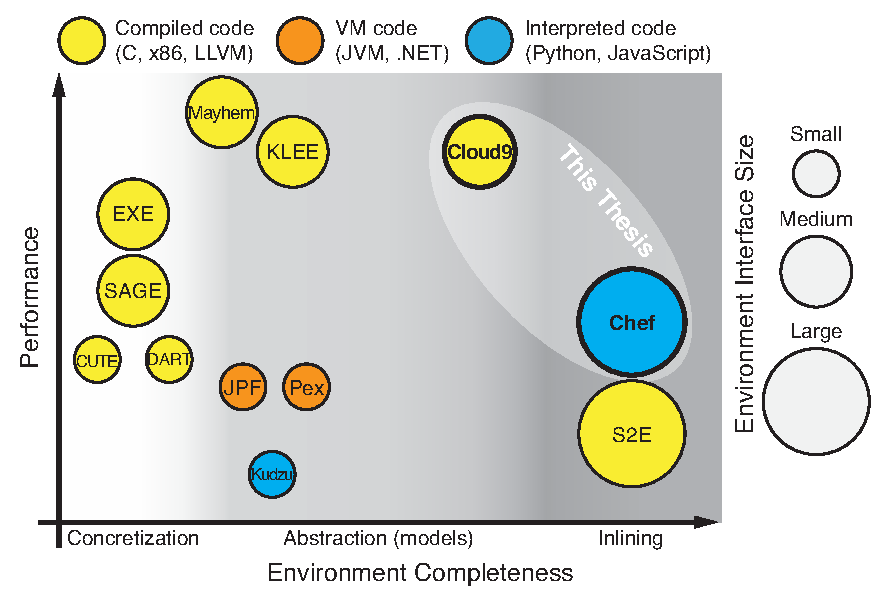
\includegraphics[width=0.8\textwidth]{relatedwork/figures/relwork-positioning}
  \caption{Qualitative comparison of most important symbolic execution engines with respect to the environment problem. X axis indicates completeness of symbolic environment, ranging from no symbolic support (concretization) to full environment inlining.  Y axis indicates relative performance of engines in terms of paths throughput, as deduced from each engine's evaluation numbers.}
  \label{fig:relwork:positioning}
\end{figure}

To efficiently handle real-world programs, symbolic execution engines need to minimize the time spent in the environment, while ensuring correct behavior in the program.
%
Existing approaches roughly fall into three categories, according to the degree of completeness in handling symbolic data going to the environment: (1) concretizing the calls to the environment (no symbolic support at all), (2) abstracting away the environment complexity through models, and (3) ``inlining'' the environment with the program.

Figure~\ref{fig:relwork:positioning} positions the existing work with respect to this classification, while qualitatively indicating the size of the environment interface targeted by the engine and the relative performance attained by each engine in its class.
%
In general, the less complete the environment support, the higher the engine performance is.  The engine performance is also influenced by the language level it targets: engines targeting complied code are typically faster than engines targeting high-level code.

Figure~\ref{fig:relwork:positioning} also shows that Chef and Cloud9 advance the state of the art by providing a better tradeoff between environment completeness and engine performance.
%
Cloud9 retains the performance of model-based environment handling, while providing an accurate operating system model that comes closer in completeness to an inlined approach.
%
On the other hand, Chef benefits from the completeness of inlining the environment---the language interpreter---with the interpreted program, while significantly improving performance over na\"{\i}ve symbolic execution.

In the rest of this section, we discuss in more detail each of the three environment approaches.

\subsection{Over-approximation (Concretization)}

A simple approach to simplifying the environment execution is to concretize the values that cross the program boundary~\cite{dart,godefroid:fuzz,klee,exe}.
%
For instance, when a symbolic value $\mu$ is passed as a parameter to an external function, the symbolic execution engine replaces the symbolic expression with a concrete example $m$.  This causes the execution to proceed linearly inside the environment.

For simple programs with limited interactions with their environment, this approach is sufficient.  However, for programs with stronger connections to the environment---e.g., maintaining open file descriptors---concretization may cause missed feasible paths and inconsistencies.

Consider the example of an environment call with symbolic arguments.  Concretization affects both the return value and the input arguments.
%
First, the return value is always concrete, which may lead the symbolic execution engine to miss value-dependent paths in the program, such as error handling.
%
Second, in order to maintain soundness, concretization introduces constraints in the path condition that bind the symbolic arguments to concrete examples (in our case, $pc_{new} := pc_{old} \wedge (\mu = m)$).  This, too, restricts the possible executions on the paths following the external call.
%
Avoiding the extra conditions might increase the coverage of the target program, at the expense of potentially introducing false executions.

A concrete environment may also introduce inconsistencies if it is shared among all execution paths~\cite{klee}.
%
This is commonly the case with non-concolic (``purely-symbolic'') execution, when the symbolic execution engine maintains all execution states as data structures in its address space.  Calls to the environment would then be passed on to the environment of the engine itself, potentially causing cross-talking between different execution paths.

\subsection{Abstraction (Modeling)}

An alternative approach to simplifying the environment is to replace its concrete implementation with a simpler one---a model---that captures its essential behavior~\cite{klee,mayhem,aeg}.
%
The model is smaller---often by orders of magnitude---than the original implementation, as it drops non-functional requirements, such as performance or fault-tolerance.  For example a key-value store database dependency of a web application could be replaced with a plain dictionary when symbolically executing it.

Symbolic execution engines implement models either by building them into the engine implementation (e.g., symbolic hardware models in S2E~\cite{s2eSystem}), or as guest code running together with the target program (e.g., the file system models in KLEE~\cite{klee}).

Although they are effective at reducing path explosion, models are expensive to write correctly and completely.  As a result, they tend to be employed only for simple or stable environment semantics, or when the model accuracy is less important (e.g., security testing~\cite{aeg}).

Cloud9 takes the modeling approach to the environment problem, when symbolically executing programs interacting with the operating system.  Cloud9 is the first to provide an accurate and efficient model for an operating system interface as complex as POSIX.  Key to our approach is to divide the model code into built-in core primitives and guest code, which helps keep the implementation simple, while covering much of the most common operating system abstractions.

\subsection{Inlining (Whole-system Analysis)}

Concretizing environment calls or writing models is unfeasible when the environment interface is large or maintains a complex state, strongly coupled to the program state.
%
For example, once loaded, a device driver typically can interact with the entire operating system kernel.  Concretizing all kernel calls would drastically reduce the exploration space, while modeling all kernel features would be expensive, especially for kernels with high internal churn, such as Linux.

For these cases, an approach that preserves correctness and completeness is to bundle the environment with the program and execute it symbolically as one target.
%
Full-VM symbolic execution engines provide this approach~\cite{s2e,bitBlaze}.

However, this approach reduces the effectiveness of symbolic execution on the original target program, due to the path explosion in the entire system, which may be orders of magnitude larger than the program.
%
To mitigate the path explosion, S2E introduces execution consistency models, which are principles of converting between symbolic and concrete values when crossing the program boundaries, in order to control the path explosion in the environment.

Chef takes the inlining approach to the environment problem, when symbolically executing programs written in interpreted languages.  Chef is the first system to use a language interpreter as a semantics provider for symbolic execution.


\subsection{Developer Control of Symbolic Environments}

The developer interface to a symbolic execution engine plays an important role in controlling its effectiveness and efficiency.
%
The best known sources of developer inputs are the search selection strategies and the injection of symbolic data in the system.
%
For example, KLEE runs command-line utilities with symbolic arguments defined using a special syntax, in line with the rest of the target arguments.  For instance, \codebit{ls -l --sym-arg 1 3} runs \codebit{ls} with the second argument symbolic, between 1 and 3 characters.  This syntax can be used to define symbolic arguments or symbolic files.

The developer control over the symbolic input was encapsulated in concepts such as parameterized unit tests~\cite{tillmann-puts}, which extend regular unit tests with parameters marked as symbolic inputs during symbolic execution.
%
Similarly, QuickCheck~\cite{quickcheck} allows writing input specifications in Haskell, which are used to instantiate inputs during random testing.

However, systems software is influenced by many other external factors, such as environment variables, system call failures, thread schedules, signal dispatch timing, and so on.
%
To address this problem, Cloud9's symbolic test interface gives extensive control over the behavior of its operating system model, such as per-file descriptor symbolic fault injection or per-socket symbolic control flow.


%%%%%%%%%%%%%%%%%%%%%%%%%%%%%%%%%%%%%%%%%%%%%%%%%%%%%%%%%%%%%%%%%%%%%%%%%%%%%%%%

\iffalse
\section{Path Explosion Mitigation}
\label{sec:relwork:pathexpl}

Dealing with the path explosion problem: grammar-based whitebox fuzzing (abstracting inputs), MultiSE (merging states), using symbolic execution friendly primitives (OVerify), underconstrained execution (dealing with a single module at a time).

Group heuristics by their goals and their inputs (the state information they use).

Search Heuristics in Symbolic Execution

Generational search in SAGE.

Eliminate or deprioritize the paths are are less likely to lead to the exploration goal.  Goes hand in hand with prioritization heuristics.

Replace two states meeting in the CFG with one that combines the memory locations and path conditions of the two.  Doesn't lead to improvements all the time, due to increased solver overhead [cite Trevor Hansen's study].

Compositionality means executing symbolically individual functions and storing the disjunction of path conditions as a function summary.  Can be computed incrementally, in response to program executions [cite demand-driven].

Addressing the solver bottleneck: query caches, memory models (Mayhem only models symbolic reads). Guarded sets in multiSE.

\section{Parallelizing Symbolic Execution}
\label{sec:relwork:parsymbex}

To our knowledge, we are the first to scalably parallelize symbolic execution to shared-nothing clusters.
%
\cite{parallelSymbex} described an extension to Java Pathfinder (JPF) that parallelizes symbolic execution by using parallel random searches on a static partition of the execution tree.  JPF pre-computes a set of disjoint constraints that, when used as preconditions on a worker's exploration of the execution tree, steer each worker to explore a subset of paths disjoint from all other workers.  In this approach, using constraints as preconditions imposes, at {\em every} branch in the program, a solving overhead relative to exploration without preconditions.  The complexity of these preconditions increases with the number of workers, as the preconditions need to be more selective.  Thus, per-worker solving overhead increases as more workers are added to the cluster.  This limits scalability: the largest evaluated program had 447 lines of code and did not interact with its environment.  Due to the {\em static} partitioning of the execution tree, total running time is determined by the worker with the largest subtree.  As a result, increasing the number of workers can even increase total test time instead of reducing it~\cite{parallelSymbex}.  \cnine mitigates these drawbacks.

There has been work on parallel model checking~\cite{parallelMurphi,distributed-spin,loadBalModelchecking,spin:multicore-modelchecking,modelCheckBDD}.  The SPIN model checker has been parallelized two-way for dual-core machines~\cite{parallelSPIN}. Nevertheless, there are currently no model checkers that can scale to many loosely connected computers, mainly due to the overhead of coordinating the search across multiple machines and transferring explicit states. \cnine uses an encoding of states that is compact and enables better scaling.

\fi

%%%%%%%%%%%%%%%%%%%%%%%%%%%%%%%%%%%%%%%%%%%%%%%%%%%%%%%%%%%%%%%%%%%%%%%%%%%%%%%%

\section{Symbolic Execution for High-level Languages}
\label{sec:relwork:interplang}

\subsection{Virtual Machine-based Languages: Java and C\#}

Beyond low-level system software, a significant amount of software is written in higher-level languages, offering features such as garbage collection, reflection, and built-in data structures.

Some of these languages, such as Java and C\#, are compiled to a lower-level bytecode representation and executed in a virtual machine.
%
The bytecode format is standardized and well-documented, which facilitates the development of dedicated symbolic execution engines for their runtimes.
%
For example, the Java PathFinder project~\cite{visser-jpf,jpf-symbex,jpf-testgen} provides a model checker and symbolic execution framework for Java bytecode.
%
Similarly, Pex~\cite{tillmann-pex} is a symbolic execution engine for .NET that has recently been distributed as part of the Visual Studio IDE.

The high-level environments pose additional challenges for symbolic execution related to the complexity of their data and execution model.  For example, symbolic program inputs can be both scalar and object-based.
%
Java PathFinder handles symbolic object inputs using a technique called generalized symbolic execution~\cite{generalized-symbex}, where symbolic objects are lazily initialized in response to the member accesses encountered during program execution.  Pex takes a similar approach for handling symbolic inputs in the .NET runtime.

\subsection{Dynamic Interpreted Languages}

The high-level languages that are never compiled, but source-interpreted, such as Python, JavaScript, Ruby, or Lua, are significantly more challenging for symbolic execution.
%
These languages have complex semantics that are under-specified, their features evolve rapidly from one version to another, and they rely on large built-in support libraries~\cite{dom2011,cutie-py,pythonReference}.
%
Building and maintaining a symbolic execution engine for these languages is a significant engineering effort.  As a result, the existing engines target only domain-specific subsets of their languages.

\paragraph{Supporting Symbolic Semantics}

Existing work addresses the problem of providing language semantics for symbolic execution in three major ways: by writing a symbolic interpreter for the language statements~\cite{nice}, executing the program concolically~\cite{cutie-py,jalangi}, and by requiring program cooperation~\cite{commuter}.

Writing a symbolic interpreter from scratch involves reconstructing the semantics for all the language constructs used by the target programs.  For example, the NICE-PySE~\cite{nice} symbolic execution engine, which is part of the NICE framework for testing OpenFlow applications, interprets the internal Python bytecode instructions generated by the interpreter when executing a program.  NICE-PySE is a Python application itself and uses the language reflection mechanisms to obtain, instrument and interpret the internal representation of the program.

The downside of writing a complete interpreter from scratch---including a symbolic execution engine---is that whenever a construct is not supported, the interpreter would halt.  To mitigate this, other engines take the concolic execution approach, where they run the real interpreter in concrete mode, and maintain in parallel the symbolic semantics of the language statements.  On the path segments where the symbolic semantics are not available, the execution can still make progress concretely, keeping the program state sound.  CutiePy~\cite{cutie-py} uses the tracing API of the Python interpreter to maintain the symbolic state in lockstep with the concrete execution.  The Jalangi dynamic instrumentation framework for JavaScript~\cite{jalangi} rewrites the target JavaScript program to insert statements for maintaining the symbolic state, similar to other symbolic execution engines for C programs~\cite{dart,cute,exe}.

In certain applications, symbolic execution is used to execute a model of a larger system, in the vein of model checking.  In this case, the model uses the specific API provided by the engine; the high-level language acts as a DSL, whose features are fully supported by the engine.
%
For example, the symbolic execution engine of the scalability testing tool Commuter~\cite{commuter} is entirely built in Python and offers an API for symbolically modeling operating system calls using the Python language.

In contrast to the existing techniques, Chef is the first system to use symbolic execution on an interpreter to symbolically execute a program written in the target interpreted language.  The closest work related to our approach is PokeEMU~\cite{hifi-lofi}, which uses symbolic execution on a reference CPU emulator to generate a test suite for checking the correctness of another emulator.  The generated test suite captures the semantics of the CPU instruction set, as implemented by the reference emulator.  However, the goal of PokeEMU is to check the implementation of the emulator, while in the case of Chef, we target the programs running in the interpreter.

\paragraph{Effectiveness of Symbolic Execution for Interpreted Languages}

Despite their shortcomings, the existing symbolic execution engines for interpreted languages have already shown promise for finding bugs, in areas where these languages are increasingly popular, such as web applications~\cite{saxena-kudzu,artzi-apollo, kiezun-ardilla}.

For instance, the Kudzu~\cite{saxena-kudzu} symbolic execution engine for JavaScript was used to detect code injection vulnerabilities.  The Apollo~\cite{artzi-apollo} engine targets PHP code to detect runtime and HTML errors, while Ardilla~\cite{kiezun-ardilla} discovered SQL injection and cross-site scripting vulnerabilities in PHP applications.
%
This potential is also confirmed by our findings with Chef, whose engines for Python and Lua discovered hangs and unexpected exceptions in popular packages (Section~\ref{sec:eval:bug-finding}).


\iffalse
\section{UNSORTED}

Closely related to symbolic execution is the concept of bounded model checking (BMC).  Instead of exploring individual execution paths and generate test cases, a BMC unfolds the control flow graph of the program and constructs a verification condition---a formula encompassing the behavior of the entire program with respect to a property to be checked.  Popular model checkers include CBMC~\cite{cbmc}, LLBMC~\cite{llbmc2012}, F-Soft~\cite{f-soft}, Magic~\cite{magic}, or Saturn~\cite{saturn}.

Beyond symbolic execution, there is substantial work done in the field of model checking and formal methods in general, which goes beyond the scope of this thesis.  We refer the interested reader to survey papers that cover the topic in more breadth~\cite{jhala2009software, woodcock2009formal}.

Black-box (random) fuzzing.

Unsound approaches.

Cooperative symbolic execution (where the program uses special APIs of the engine).

OVerify.
\fi

%% \paragraph{DART}

%% DART automatically extracts the environment interface of a C program using static analysis.  DART augment the classic random fuzzing with a dynamic analysis that collects. The advantage of concrete execution is that DART can fall back on concrete semantics when symbolic ones are not supported (e.g., multiplications) DART detects standard errors such as crashes, assertion violations, and hangs.  Dart extracts the static interface of a program, consisting of global variables and inputs to the program entry function.  It concretizes calls to library functions.

%% Initializing values in DART: either randomly, or NULL or malloced values (for pointer types).  Chef and Cloud9 leaves it to the symbolic test the job of creating inputs. The basic primitives are marking allocated buffers (or integers or strings) as symbolic.
%% Dealing with environment inconsistencies in DART: Not a problem, as programs are re-executed (so no cross-talking in paths).  But assume no side effects in the program.
%% Solver in DART: lp\_solve (linear constraints of integers and reals).
%% DART was applied on C benchmarks and an implementation of the SIP protocol, finding hundreds of crashes.
%% DART uses DFS, BFS, or random.

%% \paragraph{CUTE}
%% Unit testing using concolic execution, with memory graphs as inputs.  Separates memory constraints from scalar constraints and keeps pointer constraints simple to keep the decision procedure tractable and efficient.
%% CUTE uses DFS.
%% CUTE uses its own in-house solver, built on top of lp\_solve, which adds optimizations such as incrementality.
%% CUTE supports generation of structured data by either calling sequences of operations, or solving data structure invariants (repOk operations), similar to Korat~\cite{boyapati:korat}.
%% Used for testing data structures.

%% \paragraph{EXE}
%% Dedicated constraint solver STP, codesigned with EXE, optimized for reasoning about bitvectors and arrays, which accurately encode machine operations at good performance.
%% Has a flat view of memory.
%% Works by translating the C code to an instrumented format that includes checks for concrete/symbolic values, forks (UNIX forks), and checks for properties (memory errors, division by zero).
%% Introduced constraint optimization: caching, constraint independence.
%% DFS/BFS as search heuristics.
%% Found bugs in udhcpd, packet filters (BPF), pcre regexp library.

%% \paragraph{SAGE}~\cite{sage2012,godefroid:fuzz}
%% Used in production, during Windows development, found thousands of vulnerabilities.  Largest known deployment of symbolic execution in production.
%% Targeted large applications, binary-level.
%% Introduces the generational search heuristic for finding bugs more efficiently in an incomplete search.

%% \paragraph{KLEE}
%% Uses symbolic execution for testing real-world systems code (Coreutils, Hi-star kernel, Busybox).  They built a high-performance symbolic execution engine that finds bugs in highly tested code and achieves high coverage levels.
%% Compact state representation using COW.
%% Uses a high-performance SMT solver (STP), and optimizes interface to the solver (constraint caching, expression simplifications).
%% Handles the environment problem through a model of files (used by the Coreutils), and external calls into the host environment.
%% Handles C code by compiling and running LLVM.
%% Uses static heuristics to maximize coverage, plus standard strategies.
%% Command line interface for marking inputs symbolic.

%% \paragraph{AEG}~\cite{aeg}
%% Automated testing with the specific purpose of generating proofs of vulnerabilities (exploits), i.e., inputs that explicitly hijack the program control flow and get a shell.
%% Takes as input LLVM + binary, produces exploit.
%% Generated 16 exploits on 14 open-source projects.
%% Buggy path-first heuristic: When a path has a bug (unexploitable), it is likely that it'll exhibit more bugs that could be exploitable.
%% Loop exhaustion strategy: prioritize paths exploring maximum number of iterations.
%% Symbolic files: simplifies KLEE's interface.
%% Symbolic sockets: supplies fresh symbolic data.
%% Environment variables (concrete values, fully symbolic, failures).
%% Network, multithreading, formatting functions (about 70 system calls).  Not clear how sound the support is, nor what happens when a syscall is not supported.

%% \paragraph{Mayhem}~\cite{mayhem}
%% Finds 29 exploitable vulnerabilities in Linux and Windows programs.
%% System designed to handle efficiently (at the expense of completeness) large state spaces generated by large programs.  Efficient reasoning about symbolic memory (symbolic writes are concretized, symbolic reads are replaced with nested ite expressions).
%% Uses only binaries (no debug info needed).

%% \paragraph{Bitblaze}~\cite{bitBlaze}
%% Unified binary analysis platform, used mainly for malware analysis.

%% \paragraph{Java Path Finder}
%% \cite{jpf-symbex,jpf-testgen,generalized-symbex}.
%% Code that manipulates complex data structures.  Uses lazy initialization to instantiate data structures.
%% Built on top of the JVM.
%% Uses iterative deepening combined with DFS.
%% Model checking as a form of testing: since the program environment is typically way too large, model checking ends up being testing.
%% Can be used to either execute a repOk method and generate blackbox inputs, or do whitebox testing.

%% \paragraph{Pex}
%% Pex~\cite{tillmann-pex}.
%% Whitebox fuzzing for .NET.  Integrated in Visual Studio.  Found errors in a core .NET component.
%% Uses PUTs (parameterized unit tests)~\cite{tillmann-puts}.
%% Uses a ``meta-strategy'' that groups branches in equivalence classes, and then selects the lest chosen class.  Different sets of equivalence classes are chosen uniformly.
%% Constructing objects: run symbolically the object constructor.

%% \paragraph{Others}

%% Other older test input generation tools: \cite{genptrinputs}.

%% Korat~\cite{boyapati:korat}. Symstra~\cite{xie:symstra}.


%%% Local Variables: 
%%% mode: latex
%%% eval: (visual-line-mode)
%%% fill-column: 1000000
%%% TeX-master: "main"
%%% End:


\chapter{Primitives for Symbolic Models for Stable Operating System Interfaces}
\chaptermark{Symbolic Models for OS Interfaces}
\label{ch:cloud9}

Operating systems expose an interface that is typically stable and well documented.
%
This engenders a \emph{modeling} approach to the environment problem, which only involves the one-time effort to produce such a model.
%
However, modern operating systems are complex and provide a wide set of abstractions to programs, such as processes and threads, IPC, networking, and files.  Modeling these abstractions is challenging.

In this chapter, we present an approach to modeling the operating system interface that relies on \emph{splitting} the model in a set of most primitive operating system abstractions, on top of which a full operating system model can be implemented with reasonable effort (Section~\ref{sec:cloud9:splitmodel}).
%
We leverage the operating system model to expose hard-to-reproduce scenarios in program execution by providing a \emph{symbolic test} interface for developers (Section~\ref{sec:cloud9:symtests}).
%
Finally, we report on our experience applying these principles when building a POSIX operating system model with support for threads, processes, sockets, pipes, polling, and more (Section~\ref{sec:cloud9:posix}).


\section{Splitting Operating System Environment in Built-in Primitives and Guest Model}
\label{sec:cloud9:splitmodel}
In this section, we first present the design space of an operating system model (Section~\ref{sec:cloud9:modelspace}).  We then present our approach of a split model (Section~\ref{sec:cloud9:approach}) and how we leverage it using symbolic tests.


\subsection{The Design Space of Operating System Models}
\label{sec:cloud9:modelspace}

The goal of a symbolic model is to simulate the behavior of a real execution environment, while maintaining the necessary symbolic state behind the environment interface.
%
The symbolic execution engine can then seamlessly transition back and forth between the program and the environment.

Writing and maintaining a model can be laborious and prone to error~\cite{s2eSystem}.
%
However, for operating system interfaces, which are typically stable and well documented, investing the time to model them becomes worthwile.

Ideally, a symbolic model would be implemented as code that gets executed by the symbolic execution engine (i.e., guest-level code), substituting the implementation of the operating system and the C library.
%
Such a model can be substantially faster.  For instance, in the Linux kernel, transferring a packet between two hosts exercises the entire TCP/IP networking stack and the associated driver code, amounting to over 30 \kloc.  In contrast, our POSIX model achieves the same functionality in about 1.5 \kloc.  Requirements that complicate a real environment/OS implementation, such as performance and extensibility, can be ignored in a symbolic model.

However, not all operating system abstractions can be directly expressed as guest code.
%
In general, the problematic abstractions are those \emph{incompatible} with the execution model of the symbolic execution engine.
%
For example, providing support for multiple execution threads may not be achievable in the guest of a symbolic execution engine designed to run sequentially, unless the guest can manipulate the current stack and program counter.
%
There are other abstractions incompatible with the typical sequential single-process execution model of a symbolic execution engine, such as processes, synchronization, and shared memory.

A possible alternative is to implement the operating system model inside the symbolic execution engine, where we can define any abstraction.
%
However, this approach is undesirable.  A model built into a symbolic execution engine is significantly more expensive to produce, because the model code has to handle explicitly symbolic data and the program state.
%
For example, while a guest model of the \codebit{open} system call could directly use the string buffer of the file name passed as argument, a built-in model needs to explictly invoke read operations for the string bytes, then extract the character values from the symbolic AST expressions.


\subsection{A Split Operating System Model}
\label{sec:cloud9:approach}

Our key idea is to take the best from both worlds and provide an operating system model that is \emph{split} between a set of built-in primitives and guest-level code.
%
The built-in primitives model only the minimal operating system abstractions that would be more expensive or impossible to model at the guest level.
%
In turn, the guest-level code implements a complete operating system interface on top of these primitives.
%
In analogy to the system calls exposed by an operating system to user programs, the symbolic execution engine provides its primitives to the guest through a set of ``symbolic system calls''.

The built-in primitives provide the operating system abstractions that depend on the execution model of the symbolic execution engine.
%
The execution model includes aspects such as the program memory model and the control flow mechanisms.
%
For performance reasons, these aspects are typically encoded in the logic of the symbolic execution engine.

We identified two abstractions that are prevalent in operating systems and that should be built into the symbolic execution engine: \emph{multithreading} and \emph{address spaces}.
%
Multithreading is best provided as a built-in primitive that is integrated with the control flow mechanisms of the symbolic execution engine.
%
Similarly, providing multiple isolated address spaces is best provided by the memory model of the symbolic execution engine.  For example, the functionality needed to support address spaces (e.g., cloning) is shared with the requirements of cloning the execution state after a symbolic branch.

Many other common abstractions do not need to be built into the symbolic execution engine, but can be emulated as guest code on top of threads and address spaces.
%
Such derived abstractions include mechanisms for inter-process communication, such as sockets, pipes and files.
%
Various synchronization mechanisms, such as mutexes, semaphores, condition variables, and barriers can be provided on top of basic multi-threading primitives that put a thread to sleep and wake it up later.

We designed the support for multithreading and address spaces according to two goals: (1) minimizing the complexity of the guest code using them, and (2) capturing all possible behaviors in the real operating system, including corner-case, hard-to-reproduce scenarios.
%
The latter is especially relevant when using the symbolic execution engine to find bugs occurring in the program interaction with the operating system, as we later show in the evaluation (Section~\ref{sec:eval:bug-finding}).


\subsection{Built-in Primitives: Multithreading and Address Spaces}

We next describe the design of multithreading support and address spaces in a symbolic execution engine.

\paragraph{Multithreading}

%% A symbolic execution engine is essentially an interpreter of program statements.
%% %
To provide support for multiple threads, the symbolic execution engine maintains in each execution state a set of per-thread stacks, holding the current program location, the execution call chain, and local variables.
%
During symbolic execution, the execution alternates between the threads, governed by a thread scheduler built into the symbolic execution engine.

To simplify synchronization inside the guest model, we use a cooperative scheduler.  An enabled thread runs uninterrupted (atomically), until either (a) the thread goes to sleep, (b) the thread is explicitly preempted, or (c) the thread is terminated with a symbolic system call.

The scheduler can be configured to schedule the next thread deterministically, or to fork the execution state for each possible next thread.
%
The latter case is useful when looking for concurrency bugs.  At the same time, it can be a significant source of path explosion, so it can be selectively disabled when not needed.

The symbolic execution engine can detect hangs in the system, such as deadlocks, when a thread goes to sleep and no other thread can be scheduled.

\paragraph{Address Spaces}

In symbolic execution, program memory is typically represented as a mapping from memory locations (e.g., variables or addresses) to slots holding symbolic expressions.
%
To provide support for address spaces, we built into the symbolic execution engine support for multiple such mappings per execution state.

Each thread in the execution state is bound to one address space and each address space with its threads forms a process in the execution state.

The symbolic execution engine provides a symbolic system call for \emph{sharing} slots among multiple memory mappings.  This mechanism provides the foundation for implementing shared memory across multiple processes.
%
Shared memory can be used by the guest model to provide multiple forms of inter-process communication, such as sockets, files, and pipes.
%
For example, a socket can be modeled as a pair of memory buffers, one of each direction, shared between the client and the server processes.


\paragraph{Symbolic System Calls}

Table~\ref{table:cloud9:primitives} shows the symbolic system calls that the engine provides to the guest to support multithreading and address spaces.  We detail below the most important system calls.

\begin{table}
\centering
  
\begin{tabular}{|l|l|}
\hline
\textbf{Primitive Name} & \textbf{Description} \\
\hline
\hline
 \codebit{thread\_create(\&func)} & Create new thread that runs \codebit{func} \\
 \codebit{thread\_terminate()} & Terminate current thread \\
\hline
 \codebit{thread\_preempt()} & Preempt the current thread  \\
\hline
 \codebit{create\_wqueue()} & Create a new waiting queue \\
 \codebit{thread\_sleep(wq)} & Put current thread to sleep on waiting queue \\
 \codebit{thread\_notify(wq)} & Wake threads from waiting queue \\
\hline
\hline
 \codebit{process\_fork()} & Fork the current address space and thread \\
 \codebit{make\_shared(\&buf, size)} & Share memory across address spaces \\
\hline
\hline
 \codebit{get\_context()} & Get the current context (process and thread ID) \\
\hline
\end{tabular}

\caption{Symbolic system calls for multithreading (first block), address spaces (second block).  Third block contains introspection primitives.  The multithreading block is further divided into thread lifecycle management, explicit scheduling, and synchronization.}
\label{table:cloud9:primitives}
\end{table}

Threads are created in the currently executing process by calling \codebit{thread\_\allowbreak{}create}.  For instance, the POSIX threads (pthreads) model makes use of this primitive in its own \codebit{pthread\_create()} routine.
%
When \codebit{thread\_sleep} is called, the symbolic execution engine places the current thread on a specified waiting queue, and an enabled thread is selected for execution.
%
Another thread may call \codebit{thread\_\allowbreak{}notify} on the waiting queue and wake up one or all of the queued threads.

Cloning the current address space is available to the guest through the \codebit{process\_fork} primitive, which is used, for instance, to model the POSIX \codebit{fork()} call.
%
A memory location can be marked as shared by calling \codebit{make\_\allowbreak{}shared}; it is then automatically mapped in the address spaces of the other processes in the execution state.  Whenever a shared object is modified in one address space, the new version is automatically propagated to the others.


%%% Local Variables: 
%%% mode: latex
%%% eval: (visual-line-mode)
%%% fill-column: 1000000
%%% TeX-master: "main"
%%% End:


\section{Symbolic Tests}
\label{sec:cloud9:symtests}
Software products and systems typically have large ``hand-made'' test suites; writing and maintaining these suites requires substantial human effort.
%
\cnine aims to reduce this burden while improving the quality of testing, by offering an easy way to write ``symbolic test suites.''
%
First, a symbolic test case encompasses many similar concrete test cases into a single symbolic one---each symbolic test a developer writes is equivalent to many concrete ones.
%
Second, a symbolic test case explores conditions that are hard to produce reliably in a concrete test case, such as the occurrence of faults, concurrency side effects, or network packet reordering, dropping and delay.
%
Furthermore, symbolic test suites can easily cover unknown corner cases, as well as new, untested functionality.  In this section, we present the API for symbolic tests and illustrate it with a use case.

\subsection{Testing Platform Interface}

The \cnine symbolic testing API (Tables~\ref{table:globalapi} and~\ref{table:ioctlapi}) allows tests to programmatically control events in the environment of the program under test.
%
A test suite needs to simply include a \codebit{cloud9.h} header file and make the requisite calls.

\begin{table}
\addtolength{\tabcolsep}{-2.5pt}
{
\small
\centering
\begin{tabular}{|l|p{50mm}|}
\hline
\textbf{~~~~~Function Name} & \textbf{~~~~~~~~~~~~~~~~~~Description} \\
\hline
\cninesuffix\_make\_symbolic & Mark memory regions as symbolic \\
\hline
\cninesuffix\_fi\_enable & \multirow{2}{4cm}{Enable/disable the injection of faults} \\
\cninesuffix\_fi\_disable & \\
\hline
\cninesuffix\_set\_max\_heap & Set heap size for symbolic \codebit{malloc} \\
\hline
\cninesuffix\_set\_scheduler & Set scheduler policy (e.g., round-robin)\\
\hline
\end{tabular}
\vspace{-4pt}
\caption{\cnine API for setting global behavior parameters.}
\label{table:globalapi}
}
\end{table}

\begin{table}
\addtolength{\tabcolsep}{-2.5pt}
{
\small
\centering
\begin{tabular}{|l|p{4.8cm}|}
\hline
\textbf{~~Extended Ioctl Code} & \textbf{~~~~~~~~~~~~~~~~Description} \\
\hline
SIO\_SYMBOLIC & Turns this file or socket into a source of symbolic input \\
\hline
SIO\_PKT\_FRAGMENT & Enables packet fragmentation on this socket (must be a stream socket) \\
\hline
SIO\_FAULT\_INJ & Enables fault injection for operations on this descriptor \\
\hline
\end{tabular}
\vspace{-4pt}
\caption{\cnine extended \codebit{ioctl} codes to control environmental events on a per-file-descriptor basis.}
\label{table:ioctlapi}
}
\end{table}

\paragraph{Symbolic Data and Streams}

The generality of a test case can be expanded by introducing bytes of symbolic data.
%
This is done by calling \codebit{\cninesuffix\_make\_symbolic} to mark data symbolic, a wrapper around the SEE's primitive for injecting fresh symbolic variables in the program state.
%
%% a wrapper around \codebit{klee\_\allowbreak{}make\_\allowbreak{}symbolic}, with an argument that points to a memory region. \codebit{klee\_make\_symbolic} is a primitive provided by \klee to mark data symbolic.
%
In addition to wrapping this call, we added several new primitives to the testing API (Table~\ref{table:globalapi}). In \cnine, symbolic data can be written/read to/from files, can be sent/received over the network, and can be passed via pipes. Furthermore, the \codebit{SIO\_SYMBOLIC} \codebit{ioctl} code (Table~\ref{table:ioctlapi}) turns on/off the reception of symbolic bytes from individual files or sockets.

\paragraph{Network Conditions}

Delay, reordering, or dropping of packets causes a network data stream to be fragmented.
%
Fragmentation can be turned on or off at the socket level using one of the \cnine \codebit{ioctl} extensions.  Section~\ref{sec:eval:lighttpd} presents a case where symbolic fragmentation enabled \cnine to prove that a bug fix for the lighttpd web server was incomplete. 

\paragraph{Fault Injection}

Calls in a POSIX system can return an error code when they fail.
%
Most programs can tolerate such failed calls, but even high-quality production software misses some~\cite{lfi}. Such error return codes are simulated by \cnine whenever fault injection is turned on. 

\paragraph{Symbolic Scheduler}

\cnine provides multiple scheduling policies that can be controlled for purposes of testing on a per-code-region basis.
%
Currently, \cnine supports a round-robin scheduler and two schedulers specialized for bug finding: a variant of the iterative context bounding scheduling algorithm~\cite{chess} and an exhaustive exploration of all possible scheduling decisions.  


\subsection{Usage Example: Testing Custom Header Handling in Web Server}

Consider a scenario in which we want to test the support for a new \codebit{X-NewExtension} HTTP header, just added to a web server.
%
We show how to write tests for this new feature.

A symbolic test suite typically starts off as an augmentation of an existing test suite;
%
in our scenario, we reuse the existing boilerplate setup code and write a symbolic test case that marks the extension header symbolic. Whenever the code that processes the header data is executed, \cnine forks at all the branches that depend on the header content. Similarly, the request payload can be marked symbolic to test the payload-processing part of the system:

\begin{verbatim}
   char hData[10];
   cloud9_make_symbolic(hData);
   strcat(req, "X-NewExtension: ");
   strcat(req, hData);
\end{verbatim}

The web server may receive HTTP requests fragmented in a number of chunks, returned by individual invocations of the \codebit{read()} system call---the web server should run correctly regardless of the fragmentation pattern.
%
To test different fragmentation patterns with \cnine, one simply enables symbolic packet fragmentation on the client socket:
\begin{verbatim}
   ioctl(ssock, SIO_PKT_FRAGMENT, RD);
\end{verbatim}

To test how the web server handles failures in the environment, we can ask \cnine to selectively inject faults when the server reads or sends data on a socket by placing in the symbolic test suite calls of the form:
\begin{verbatim}
   ioctl(ssock, SIO_FAULT_INJ, RD | WR);
\end{verbatim}
\cnine can also enable/disable fault injection globally for all file descriptors within a certain region of the code using calls to \codebit{\cninesuffix\_fi\_\allowbreak{}enable} and \codebit{\cninesuffix\_fi\_\allowbreak{}disable}. For simulating low-memory conditions, \cnine provides a \codebit{\cninesuffix\_set\_\allowbreak{}max\_heap} primitive, which can be used to test the web server with different maximum heap sizes.

%%% Local Variables: 
%%% mode: latex
%%% eval: (visual-line-mode)
%%% fill-column: 1000000
%%% TeX-master: "main"
%%% End:


\section{Case Study: A Symbolic POSIX Interface Model}
\label{sec:cloud9:posix}
We used the SEE system call interface to build a model for the POSIX interface.
%
In this section, we describe the key design decisions involved in building the model, and we illustrate the use of the symbolic system call interface.
%
This also serves as an example for building additional models on top of the \cnine symbolic system call interface.

The POSIX model uses shared memory structures to keep track of all system objects (processes, threads, sockets, etc.).
%
The two most important data structures are stream buffers and block buffers, analogous to character and block device types in UNIX.  Stream buffers model half-duplex communication channels: they are generic producer-consumer queues of bytes, with support for event notification to multiple listeners.  Event notifications are used, for instance, by the polling component in the POSIX model.  Block buffers are random-access, fixed-size buffers, whose operations do not block; they are used to implement symbolic files.

The symbolic execution engine maintains only basic information on running processes and threads: identifiers, running status, and parent--child information.
%
However, the POSIX standard mandates additional information, such as open file descriptors and permission flags. This information is stored by the model in auxiliary data structures associated with the currently running threads and processes. The implementations of \codebit{fork()} and \codebit{pthread\_create()} are in charge of initializing these auxiliary data structures and making the appropriate symbolic system calls.

Modeling synchronization routines is simplified by the cooperative scheduling policy:
%
no locks are necessary, and all synchronization can be done using the sleep/notify symbolic system calls, together with reference counters.  Figure~\ref{fig:mutexcode} illustrates the simplicity this engenders in the implementation of pthread mutex lock and unlock.

\begin{figure}
  \centering
  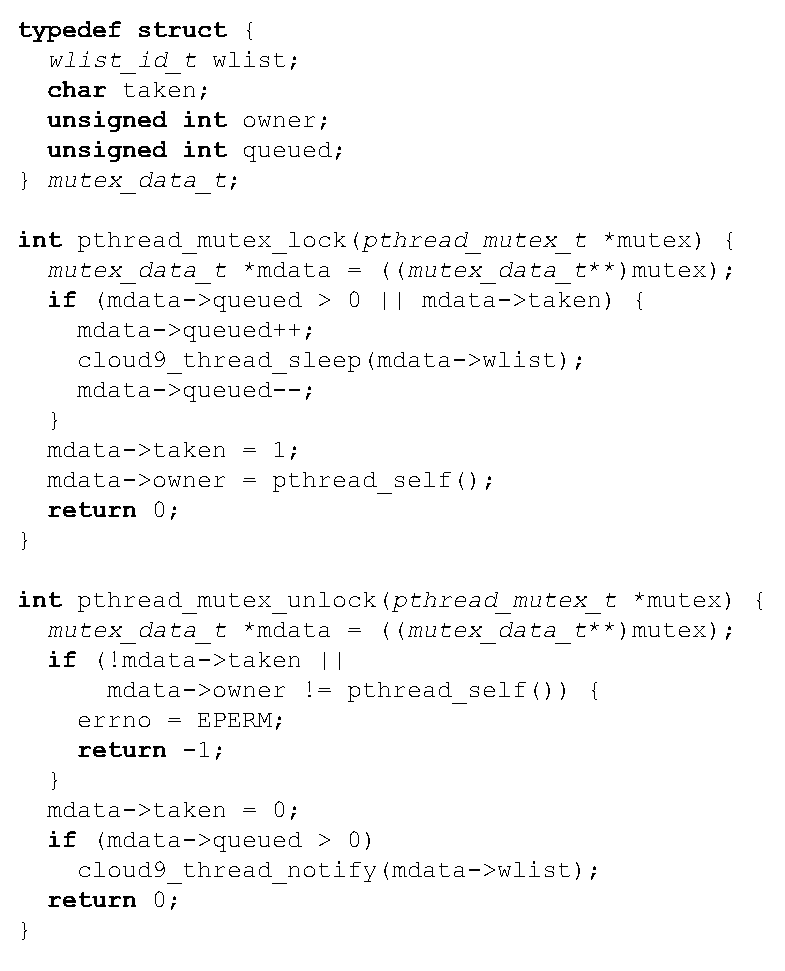
\epsfig{file=cloud9/figures/mutex-model.eps, width=3.2in}
  \caption{Example implementation of pthread mutex operations in \cnine's POSIX environment model.}
  \label{fig:mutexcode}
\end{figure}

\cnine uses most of \klee's file model semantics.
%
In particular, one can either open a symbolic file (its contents comes from a symbolic block buffer), or a concrete file, in which case a concrete file descriptor is associated with the symbolic one, and all operations on the file are forwarded as external calls on the concrete descriptor. 

\begin{figure}
  \centering
  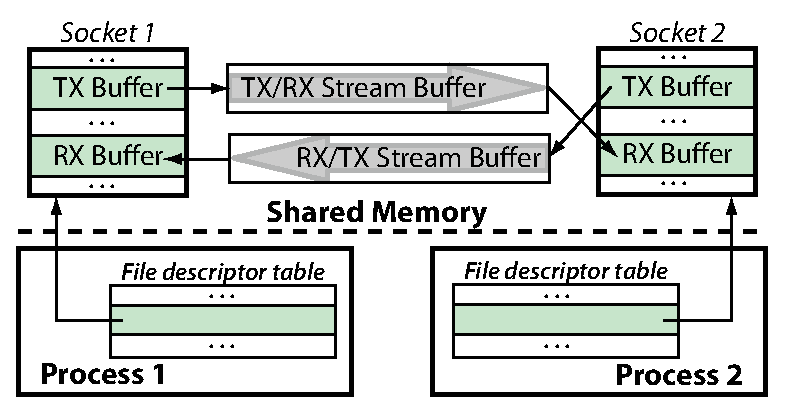
\epsfig{file=cloud9/figures/network-model.eps, width=4.0in}
  \caption{A TCP network connection is modeled in \cnine using TX and RX buffers implemented as stream buffers.}
  \label{fig:networkmodel}
\end{figure}

In addition to file objects, the \cnine POSIX model adds support for networking and pipes.
%
Currently, the TCP and UDP protocols are supported over IP and UNIX network types. Since no actual hardware is involved in the packet transmission, we can collapse the entire networking stack into a simple scheme based on two stream buffers (Figure~\ref{fig:networkmodel}). The network is modeled as a single-IP network with multiple available ports---this configuration is sufficient to connect multiple processes to each other, in order to simulate and test distributed systems. The model also supports pipes through the use of a single stream buffer, similar to sockets.

The \cnine POSIX model supports polling through the \codebit{select()} interface.
%
All the software we tested can be configured to use \codebit{select()}, so it was not necessary to implement other polling mechanisms.  The \codebit{select()} model relies on the event notification support offered by the stream buffers that are used in the implementation of blocking I/O objects (currently sockets and pipes).

The constraint solver used in \cnine operates on bit vectors; as a result, symbolic formulas refer to contiguous areas of memory.
%
In order to reduce the constraint solving overhead, we aim to reduce the amount of intermixing of concrete and symbolic data in the same memory region.  Thus, \cnine's POSIX model segregates concrete from symbolic data by using static arrays for concrete data and linked lists (or other specialized structures) for symbolic data.  We allocate into separate buffers potentially-symbolic data passed by the tested program through the POSIX interface.

In order to enable testing the systems presented in the evaluation section (Section~\ref{sec:eval:targets}), we had to add support for various other components: IPC routines, \codebit{mmap()} calls, time-related functions, etc.
%
Even though laborious, this was mostly an engineering exercise, so we do not discuss it further.

Finally, in some cases, it is practical to have the host OS handle parts of the environment via \emph{external calls}.
%
These are implemented by concretizing the symbolic parameters of a system call before invoking it from symbolically executing code. Unlike \cite{dart,klee,exe}, \cnine allows external calls \emph{only} for stateless or read-only system calls, such as reading a system configuration file from the \codebit{/etc} directory.  This restriction ensures that external concrete calls do not clobber other symbolically executing paths.

%%% Local Variables: 
%%% mode: latex
%%% eval: (visual-line-mode)
%%% fill-column: 1000000
%%% TeX-master: "main"
%%% End:


\section{Summary}

Operating systems expose a complex stateful interface to user programs.
%
In this chapter, we showed a way to provide an operating system environment for symbolic execution by employing a split operating system model.  A core set of primitives built into the symbolic execution engine serves as a base, on top of which a full operating system interface is emulated inside the guest.
%
As few as two primitives are sufficient to support complex operating system interfaces: threads  with synchronization and address spaces with shared memory.
%
We showed how to use the core primitives to provide an accurate model of the POSIX interface.
%
Our POSIX model includes extensions that developers can use in symbolic tests to control non-deterministic operating system events, such as thread scheduling and network flow control, in order to increase the coverage in the target programs.

%%% Local Variables: 
%%% mode: latex
%%% eval: (visual-line-mode)
%%% fill-column: 1000000
%%% TeX-master: "main"
%%% End:


\chapter{Using Interpreters as Specifications for Fast-changing Languages}
\chaptermark{Using Interpreters as Specifications}
\label{ch:chef}
In the previous chapter, we showed how to efficiently create accurate models for operating system interfaces, which are stable and well documented.
%
For interfaces with unstable and incomplete specifications, such as those of dynamic languages, such as Python, Ruby, or JavaScript, the environment problem mandates a different approach.
%
In this chapter, we present \chef, a symbolic execution platform for interpreted languages that relies on using the language interpreter as an ``executable specification''.

%% \newcommand{\true}{\ensuremath{\mathrm{true}}}
\newcommand{\pc}{\ensuremath{\mathit{pc}}}
\newcommand{\hlhlt}[1]{\textcolor{blue}{#1}}
\newcommand{\concat}{\ensuremath{\oplus}}

\begin{algorithm}
  \SetCommentSty{textrm}
  \KwIn{Initial location $\ell_0$.}
  \KwData{Low-level state set $w$ and high-level tree $T$, represented as set of paths.}
  \BlankLine
  $w := \{ (\ell_0, \hlhlt{[L_0]}, \true, \lambda v .v) \}$\;
  $\hlhlt{T := \{ [L_0] \}}$; $\hlhlt{W := \{ [L_0] \}}$\;
  \While{$w \neq \varnothing$}{
    $(\ell, \hlhlt{\overline{P}}, \pc, s) := \hlhlt{\mathit{pickNextLL}(w, T, W)}$;  $S := \varnothing$\;
    \tcp{Symbolically execute the next instruction}
    \Switch{$\mathit{instr}(\ell)$}{
      \Case(\hfill// assignment\hspace*{4cm}){$v := e$}{
        $S := \{(\mathit{succ}(\ell), \hlhlt{\overline{P}}, \pc, s[v \mapsto \mathbf{eval}(s, e)])\}$\;
      }
      \Case(\hfill// conditional jump\hspace*{4cm}){$\mathsf{if}(e) \; \mathsf{goto} \; \ell'$}{
        \If{$\mathit{follow}(\pc \wedge s \wedge e)$}{
          $S := \{ (\ell', \hlhlt{\overline{P}}, \pc \wedge e, s) \}$\;
        }
        \If{$\mathit{follow}(\pc \wedge s \wedge \neg e)$}{
          $S := S \cup \{ (\mathit{succ}(\ell), \hlhlt{\overline{P}}, \pc \wedge \neg e, s) \}$\;
        }
      }
      \hlhlt{\Case(\hfill// high-level program location\hspace*{4cm}){$\mathsf{hlpc}(L')$}{
        $S := \{(\mathit{succ}(\ell), \overline{P} \concat [L'], \pc, s)\}$\;
        \tcp{Merge path into the execution tree}  
        $T := T \sqcup \overline{P}$\;
      }}
      \Case(\hfill// program halt\hspace*{4cm}){$\mathsf{halt}$}{
        \hlhlt{\emph{Do nothing}}\;
      }
    }
    $w := w \cup S$\;
  }
  \vskip 5.0pt
  \caption{The low-level symbolic execution algorithm, as presented in~\cite{state-merging}, modified for maintaining high-level location information.}
  \label{alg:chef:ll-symbex}
\end{algorithm}


\begin{algorithm}
  \SetCommentSty{textrm}
  \SetKwProg{Fn}{Function}{}{end}
  \SetKwFunction{PickNext}{pickNextLL}
  \SetKw{Break}{break}
  \Fn{\PickNext{w, T}}{
    \KwData{Low-level state set $w$, high-level execution tree $T$, and high-level state set $W$.}
    \KwResult{Removes from $w$ a low-level state and returns it.}
    \BlankLine
    \While{$W \neq \varnothing$}{
      $\overline{P} := \mathit{pickNextHL}(W)$\;
      \If{$\neg canProgress(\overline{P})$}{
        $W := W \cup \{\overline{P}\}$\;
        \Break\;
      }
      \tcp{Add path successors in tree $T$}
      $W := W \cup \mathit{succ}(\overline{P}, T)$\;
    }
    \If{$W = \varnothing$}{
      \tcp{Pick low-level state aiming to discover new high-level path}
      \Return{$\mathit{pickNextLLGlobal}(w)$}\;
    }
    \tcp{Pick low-level state to make progress on path $\overline{P}$}
    \Return{$\mathit{pickNextLLLocal}(w, \overline{P})$}\;
  }
  \caption{The low-level state selection strategy, which implements the high-level symbolic execution algorithm.}
  \label{alg:chef:ll-strategy}
\end{algorithm}


%%% Local Variables: 
%%% mode: latex
%%% eval: (visual-line-mode)
%%% fill-column: 1000000
%%% TeX-master: "main"
%%% End:


\section{System Overview}
\begin{figure}
  \centering
  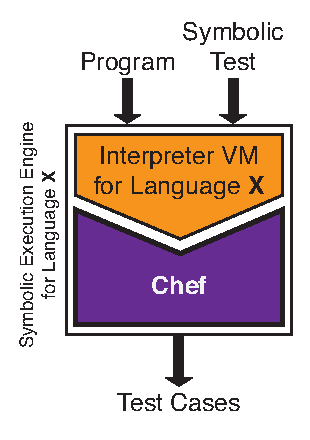
\includegraphics[width=0.3\textwidth]{chef/figures/usage-model}
  \caption{Overview of \chef's usage.}
  \label{fig:chef:overview}
\end{figure}

\chef is a platform for language-specific symbolic execution.
%
Provided with an interpreter environment, which acts as an executable language specification, \chef becomes a symbolic execution engine for the target language (see Figure~\ref{fig:chef:overview}).
%
The resulting engine can be used like a hand-written one, in particular for test case generation.  When supplied with a target program and a symbolic test case (also called test driver or test specification in the literature), the \chef engine outputs a set of concrete test cases, as shown in Figure~\ref{fig:chef:overview}.

\paragraph{Example}

\begin{figure}
  \centering
  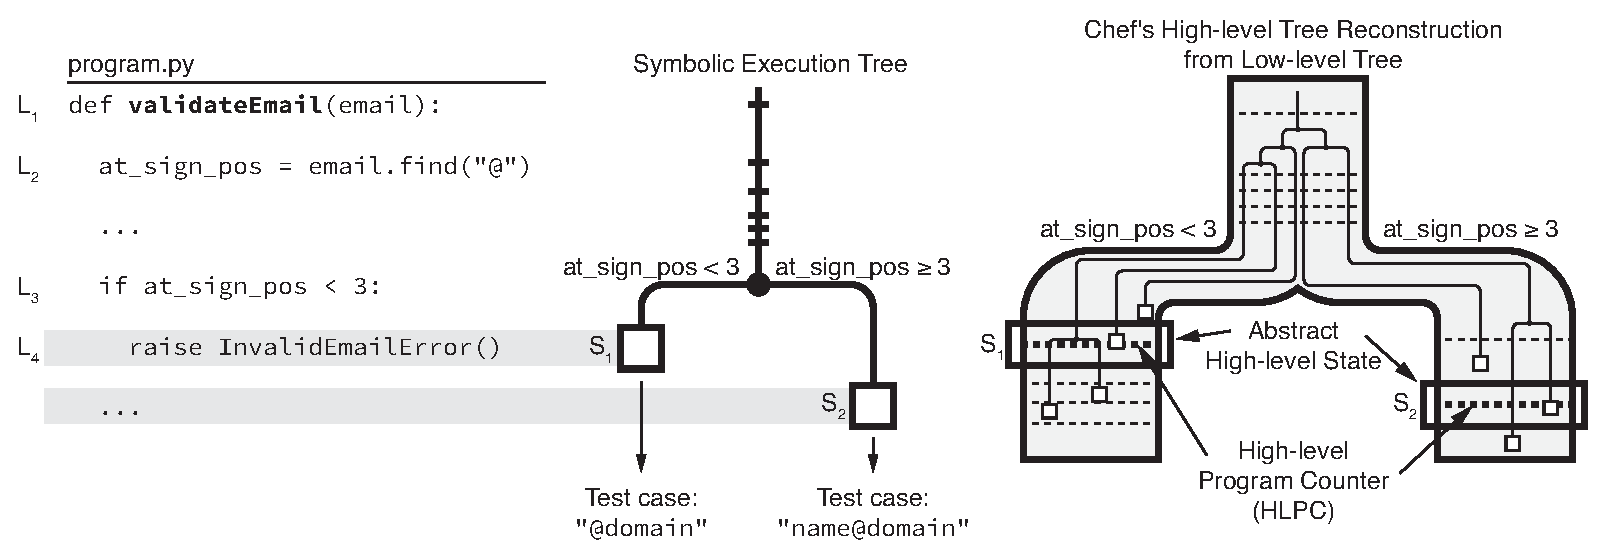
\includegraphics[width=\textwidth]{chef/figures/running-example}
  \caption[Example of Python code that validates an e-mail address given as a string with corresponding symbolic execution tree and mapping of interpreter paths to program paths.]{Example of Python code that validates an e-mail address given as a string (left) with corresponding symbolic execution tree (center) and mapping of interpreter paths to program paths (right).  Marks on the execution path indicate program statements.}
  \label{fig:chef:running-example}
\end{figure}

We illustrate the functionality of \chef using the Python example in Figure~\ref{fig:chef:running-example} (left).
%
The function \codebit{validateEmail} receives an e-mail address string and raises an exception if the address is malformed.
%
We symbolically execute the function using a \chef engine obtained by plugging the Python interpreter.

The \chef engine receives the Python program together with a symbolic test that marks the \codebit{email} input argument as symbolic.

\chef constructs the symbolic execution tree of the program, as shown in Figure~\ref{fig:chef:running-example} (center).
%
The paths in the tree are sequences of program locations, corresponding to a statement or bytecode instruction.  Branches can occur explicitly at control flow statements (as in our example), or implicitly through exceptions.

\chef prioritizes execution states according to a pluggable search strategy (see Section~\ref{sec:intro:symbex}).
%
There are two execution states in our example: $S_1$, which executes the exception path, and $S_2$, which executes the normal path.
%
A strategy may randomly select states to uniformly cover the set of possible paths, or it may favor the states that are triggering exceptions in the program, such as $S_1$.

At the end of each execution state, \chef generates a concrete string value for the \codebit{email} argument, which constitutes a test case.
%
Each test case takes the Python program along the same execution path, when replayed in the same interpreter.


\paragraph{The Interpreter as Language Specification}

\chef is built on top of the S2E analysis platform~\cite{s2eSystem}, which symbolically executes the interpreter environment \emph{at binary level}.
%
The interpreter environment is a virtual machine that bundles the interpreter, a testing library, the operating system, and other user programs.
%
For example, to symbolically execute the program in Figure~\ref{fig:chef:running-example},  \chef runs the interpreter by invoking \codebit{./python program.py} inside the virtual machine.

The resulting engine is a correct symbolic execution engine for the target language \emph{as defined by the interpreter}.
%
It is fully precise and theoretically complete, i.e., it will not explore infeasible paths and will eventually explore all paths.\footnote{The usual limitations of symbolic execution engines apply: completeness holds only under the assumption that the constraint solver can reason about all generated path conditions, and it is understood that exhaustive exploration is usually impractical in finite time.}

%%% Local Variables: 
%%% mode: latex
%%% eval: (visual-line-mode)
%%% fill-column: 1000000
%%% TeX-master: "main"
%%% End:


\section{\chef's Architecture as Adapter Between Engine Interfaces}
\begin{figure}
  \centering
  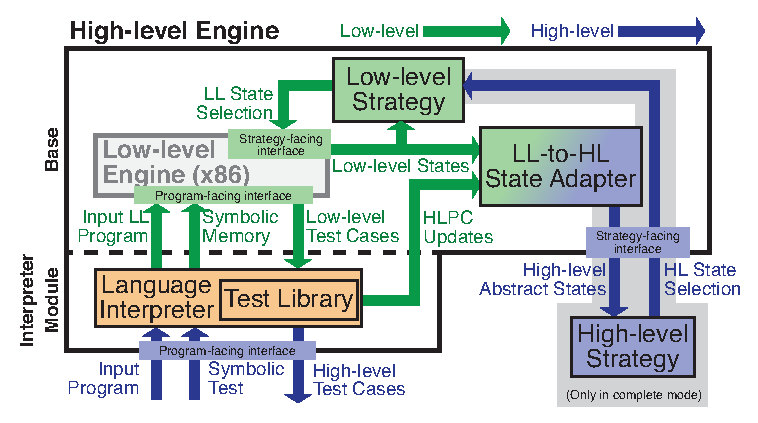
\includegraphics[width=1.0\textwidth]{chef/figures/iface-adapter}
  \caption{The architecture of \chef.}
  \label{fig:chef:arch}
\end{figure}

\chef acts as an adapter between two symbolic execution engine interfaces:
%
the user-facing \emph{high-level} engine interface that receives the target program and the internal \emph{low-level} binary engine that runs the interpreter.
%% %
%% The main function of \chef is to prioritize the low-level interpreter states that maximize the effectiveness of test case generation at the high-level.

The interface of a symbolic execution engine consists of a program-facing part and a strategy-facing part.
%
Through the program-facing part, the symbolic execution engine receives the program and the symbolic test and outputs test cases.
%
Through the strategy-facing part, the engine sends the active execution states to an external state selection strategy and receives the choice of the next state to run (see Section~\ref{sec:intro:symbex}).


Figure~\ref{fig:chef:arch} shows the architecture of \chef, consisting of the base and an interpreter module.
%
The base contains the \emph{low-level} binary symbolic execution engine (S2E) that runs the interpreter, the low-level state selection strategy, and an \emph{adapter} that creates high-level program paths based on the observed low-level interpreter paths.
%
An external high-level strategy communicates with the base to provide the next high-level state to run.

The interpreter module contains the language interpreter, which provides the implicit semantics of the language.

Both the inner and the outer interfaces of \chef expose the program-facing and the strategy-facing part.
%
The inner engine operates with machine-level abstractions: it runs a binary program---the interpreter---and marks memory bytes as symbolic inputs.  During symbolic execution, it generates paths through the interpreter binary, prioritized by the low-level strategy.
%
The outer engine operates with corresponding high-level abstractions: it runs an interpreted program and marks objects, instead of bytes, as symbolic.  During execution, it generates paths through the high-level program.

The interpreter module \emph{by construction} adapts the program-facing part of the two interfaces, as shown in Figure~\ref{fig:chef:arch}.
%
Reusing the interpreter provides substantial savings in terms of development effort.  For instance, the Python interpreter has over 400 KLOC; a hand-written symbolic execution engine would reimplement from scratch the same language semantics in an implementation of the same order of magnitude.

The main task left for \chef is to provide the low-level strategy for choosing the interpreter paths that maximize \chef's effectiveness as a high-level symbolic execution engine.
%
We discuss this aspect in the next section.

%%% Local Variables: 
%%% mode: latex
%%% eval: (visual-line-mode)
%%% fill-column: 1000000
%%% TeX-master: "main"
%%% End:


\section{From Low-level to High-level Symbolic Execution Semantics}
\paragraph{The High-level Symbolic Execution Tree}

Consider again the example in Figure~\ref{fig:chef:running-example}.
%
On line $L_2$, the \codebit{find} method executes as a single statement at the Python level, but internally, the interpreter forks hundreds of alternate states, for each possible path in the implementation of the substring searching algorithm.
%
Some of these paths lead the program to take the branch at line $L_4$ and raise the exception, while the others continue the execution normally.
%
\chef groups the low-level interpreter paths into their corresponding high-level program paths (right side of Figure~\ref{fig:chef:running-example}) and reports a single test case per high-level path.

%% \chef builds the high-level symbolic execution tree of the program by aggregating the low-level execution paths it observes in the interpreter.
%% %

To group the low-level paths into high-level paths, \chef tracks the program location---the \emph{high-level program counter} (HLPC)---of each low-level interpreter state.
%
The HLPC values are opaque to \chef.  Their concrete semantics depend on the language and the interpreter.  For example, for interpreters that compile programs to an intermediate bytecode representation, the HLPC can be the address in memory of each bytecode instruction (Section~\ref{sec:chef:hlcf}).

The low-level paths that have the same sequence of HLPC values map to the same high-level path.
%
This results in a high-level symbolic execution tree that ``envelops'' the low-level symbolic execution tree of the interpreter.

\paragraph{Abstract High-level States}

The expansion of the high-level tree is governed by the high-level strategy.
%
The strategy expects a set of high-level states to choose from, as per the general contract of the strategy interface.  There is one high-level state per path, reflecting the progress of the execution on that path.
%
However, it is the \emph{low-level} execution states that determine the high-level paths, as previously explained.
%
Moreover, there could be \emph{several} low-level states on the path.
Intuitively, each low-level state executes a ``slice'' of the entire high-level path, and may reside at any HLPC location on the path.


To adapt between the two interface levels, \chef introduces the notion of \emph{abstract high-level state}.
%
Each high-level path has exactly one abstract high-level state, which resides at a HLPC location on the path.
%
When a new high-level path branches, its abstract high-level state starts at the beginning of the path.
%
The state subsequently advances to the next HLPC when it is selected for execution, and it is terminated when it reaches the end of the path.


An abstract high-level state may only advance to the next HLPC when the underlying low-level states on the path have executed enough of the program statement.
%
\chef provides two policies that govern this relationship, called \emph{state completeness models}.  They are discussed in detail in the next section.


We call an abstract high-level state \emph{blocking}, when it cannot make progress on the path, according to the state completeness model used.
%
When the abstract state is blocking, the low-level strategy selects for execution low-level states that unblock the abstract state.

\paragraph{The Low-level State Selection Workflow}

By using abstract high-level states, the selection of low-level states becomes a two-stage process, as shown in the architecture diagram (Figure~\ref{fig:chef:arch}).
%
First, the low-level engine reports its execution states to an \emph{adapter} component, which maintains the high-level symbolic execution tree and the abstract high-level states.
%
The state adapter reports the abstract high-level states to the high-level strategy, which decides the next high-level state---and therefore path---to explore.
%
If the state completeness model allows the state to advance on the path, the state adapter updates the HLPC directly.
%
If not, the high-level strategy communicates its choice to the low-level strategy, which selects a low-level state on the path that helps unblock the abstract high-level state.


This state selection process both (a) provides an adapter mechanism for selecting \emph{low-level} interpreter states for execution based on a \emph{high-level} strategy, and (b) still preseves the high-level abstractions by hiding the interpreter and its states.


The abstract high-level states only contain the current HLPC and a path condition.
%
Unlike the low-level states, they do not include program data, as its semantics are language-dependent.
%
Instead, the program data is implictly encoded and distributed across the low-level states on the path and manipulated by the interpreter.

%%% Local Variables: 
%%% mode: latex
%%% eval: (visual-line-mode)
%%% fill-column: 1000000
%%% TeX-master: "main"
%%% End:


\section{Trading Precision for Efficiency with State Completeness Models}
\label{sec:chef:completeness-models}
The state adapter uses the state completeness model to determine whether an abstract high-level state blocks or can be advanced to the next HLPC on its path.
%
\chef provides two completeness models: \emph{partial} and \emph{complete}.
%
The two models provide different trade-offs between the precision of controlling the high-level execution and the expected path throughput in the high-level symbolic execution engine.

\begin{figure}
  \centering
  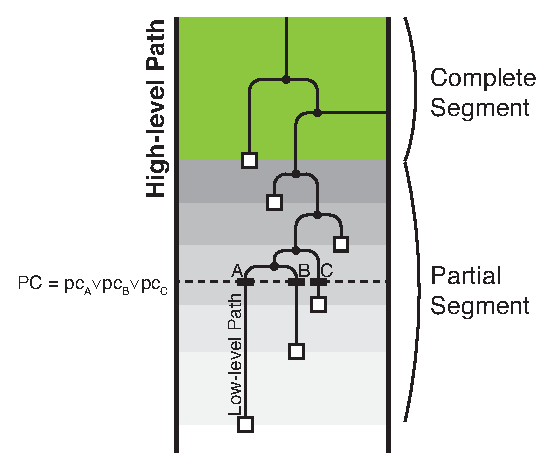
\includegraphics[width=3in]{chef/figures/path-segments}
  \caption{High-level execution path, segmented according to completeness of exploration by the low-level paths.}
  \label{fig:chef:path-segments}
\end{figure}

Before we present the two models, we introduce the notion of \emph{local path condition} and \emph{path segments} (Figure~\ref{fig:chef:path-segments}).

\paragraph{Local Path Condition}

We define the local path condition of a high-level path at a given HLPC location as the disjunction of the path conditions of all low-level states that traversed the HLPC location, \emph{at the moment the interpreter started executing the statement at the given HLPC}.
%
Each statement on the high-level path has a local path condition.

The local path condition of a HLPC location is \emph{complete} if all low-level states on the path are located after the statement.
%
This means that there is no further interpreter execution that would reach the HLPC location.
%
Hence, a complete local path condition describes \emph{all} inputs that take the program along the given high-level path.

Conversely, if there exist low-level states that are located before the HLPC location on the path, its local path condition is \emph{partial}.
%
The local path condition shown in Figure~\ref{fig:chef:path-segments} is partial, because there are three states before it.
%
Any of them could reach the program at that location and augment the possible program executions on the path.

\paragraph{Path Segments}

We divide a high-level execution path in two segments, according to the completeness of the local path conditions of its HLPC locations:
\begin{itemize}
\item The \emph{complete segment} consists of all locations traversed by all low-level states on the path.
%
The segment starts at the beginning of the path and ends at the HLPC of the least advanced low-level state on the path (the green block in Figure~\ref{fig:chef:path-segments}).
\item The \emph{partial segment} consists of the rest of the path, which contains the locations traversed by at least one, but not all, low-level states on the path.
%
The segment starts with the least advanced low-level state on the path and ends at the leading state on the path.  Figure~\ref{fig:chef:path-segments} shows the partial segment in nuances of gray, according to the degree of local path completeness.
\end{itemize}

Each HLPC location on the high-level path transitions from partial to complete.
%
In case a high-level path consists of a single low-level path, the transition goes directly to complete and the partial segment is empty.

\paragraph{The State Completeness Models}

The partial and completeness models are defined with respect to the path segments on which the abstract high-level states are allowed to reside.

In the partial model, the abstract high-level states are allowed to reside anywhere on the high-level execution path, i.e., on both its complete and partial segment.
%
On the other hand, in the complete model, the abstract high-level states are only allowed on complete segments.

This difference creates substantial divergences in the properties of the two models, which we discuss next.

\subsection{Partial High-level Execution States}

In the partial model, the abstract high-level states are allowed to reside anywhere on the high-level execution path.
%
Therefore, the states block only at the last HLPC location on the path.

The low-level strategy unblocks the abstract high-level states by selecting for execution the leading low-level state on the path.
%
Therefore, the cost of unblocking the state is relatively low: only one low-level state from the entire path is required, which amounts to simpler symbolic expressions and faster solver queries.

On the other hand, in the partial model, the execution of the abstract high-level state may miss feasible high-level branches.
%
This is because the local path condition of the abstract state is incomplete, and therefore may not include the low-level executions that diverge into other high-level paths at branching points.
% GIVE EXAMPLE
% For interpreted languages, many instructions can potentially be branching points, either as explicit branch instructions, or as statements that may throw exceptions.

As a result, the high-level strategy can only exercise control over high-level paths \emph{already discovered}.
%
New high-level paths are discovered only as the low-level strategy repeatedly selects low-level states for execution on the existing paths.


\subsection{Complete High-level Execution States}

In the complete model, the abstract high-level states can only reside on the complete path segment.
%
The states block at the first low-level state encountered on the path, before entering the partial segment.

The low-level strategy unblocks the abstract high-level states by executing all low-level states that reside on the next statement on the path.
%
Therefore, compared to the partial mode, the cost of unblocking the state is significantly higher.

However, in the complete model, the feasibility of all branching instructions traversed by the abstract high-level states are decided, as the local path conditions are complete.
%
In turn, the high-level execution strategy has knowledge of all paths forking off the currently discovered ones, and can influence the exploration ordering.

\subsection{Choosing Between the Two Models}

\newcommand{\goodcolor}{\cellcolor{LimeGreen}}
\newcommand{\badcolor}{\cellcolor{Lavender}}

\begin{table}
  \centering
  \small
  \begin{tabular}{r c c}
    High-level State Model & \textbf{Partial} & \textbf{Complete}               \\
    \hline
    \noalign{\smallskip}
    Location (HLPC) & Complete and partial segments & Complete segments only    \\
    Path Condition  & Incomplete                    & Complete                  \\
    Strategies      & Only at low level             & Both high- and low-level  \\
    \noalign{\smallskip}
    \hline
    \noalign{\smallskip}
    Efficiency (state cost) & \goodcolor One low-level state   & \badcolor All low-level states      \\
    Precision       & \badcolor Low (no branch feasibility)   & \goodcolor Full control over states  \\
  \end{tabular}
  \caption{Comparing partial and complete high-level state models in \chef.}
  \label{tab:chef:hl-states}
\end{table}

Table~\ref{tab:chef:hl-states} summarizes the trade-offs between the partial and complete state models.
%
On the one hand, the partial state model lacks precision, as it does not expose to the high-level engine interface any pending high-level states, but gains efficiency, as it uses as little as one low-level state to explore a high-level path, once discovered.
%
On the other hand, the complete state model provides full precision, as it is able to determine all feasible branches along each explored path, at the expense of a more costly path exploration.

Both state models are useful for symbolic execution.
%
Fundamentally, both models handle the same low-level state information coming from the underlying symbolic execution engine.  The difference relates to how the data is organized into execution paths and test cases.

The partial state model works best for exploratory automated test case generation.
%
The low-level strategy aims to discover new high-level paths, which are then executed efficiently using a single low-level state, which gives the test case for the path.

The precise state model is more appropriate for directed test case generation and exhaustive testing.
%
The high-level strategy works with the low-level strategy to focus the exploration on particular high-level paths.  At the same time, the decoupling between the two strategies opens up optimization opportunities at the low-level, such as state merging, which increases the efficiency of exhaustive testing.

%% This limitation makes it more difficult to build analyses that read the program state, including search selection strategies, such as the coverage-optimized strategy in \klee~\cite{klee}.
%% %
%% However, the high-level state remains implicitly encoded in the low-level interpreter state and can be accessed by executing code in the target language, by the interpreter runtime.  Therefore, a possible workaround is to split the analysis in a language-independent part, running as part of Chef, and a language-dependent part, written in the target language and running as an interrupt in the interpreter context, whenever it is needed.

%% Determining the positions of a high-level state on its high-level path is not as clear-cut.
%% %
%% The low-level states on the high-level path may reside at different points on the path, so there is no straightforward mapping from them to the high-level state.

%% The leading low-level state of the high-level path defines the boundary between the partial and undiscovered segment, while the trailing state on the path defines the boundary between the completed and partial segment.

%% %
%% In other words, the goal of the system becomes that of maximizing the high-level path yield for the set of low-level paths explored.
%
%% However, as executing low-level paths is efficient, in practice, a judicious state selection strategy can effectively discover significantly more high-level paths compared to naively choosing paths at random (Section~\ref{sec:xxx}).


%%% Local Variables: 
%%% mode: latex
%%% eval: (visual-line-mode)
%%% fill-column: 1000000
%%% TeX-master: "main"
%%% End:


\section{Path Prioritization in The Interpreter}
\label{sec:chef:strategies}
%% An interpreted program conceptually executes both on a high level---the level of the target language---and a low level---the level of the interpreter.
%% %
%% The low-level program path is the sequence of machine instructions from the interpreter binary, including the code for internal bookkeeping (e.g., details of reference counting and garbage collection).

%% In practice, the number of low-level paths mapping to the same high-level path can be very large.  Their number increases roughly exponentially with the number of internal interpreter branches occurring along the high-level path, caused by implementation details, such as garbage collection or reference counting. \stefan{Maybe remove the reference to exponential growth, and give instead an example.}
%% %
%% To mitigate the path explosion along high-level paths, \chef employs state prioritization heuristics, which are discussed in Section~\ref{sec:xxx}.

%% Third, a high-level branch can occur \emph{at any point after} the low-level paths branches inside the interpreter.  This impacts the effectiveness of the heuristics aiming at discovering new high-level paths through the interpreter.
%% %
%% For example, the interpreter may implement a branching statement in two distinct steps: a comparison and a conditional jump.  In Figure~\ref{fig:xxx}, three low-level paths fork within the single HLPC location for \codebit{email.find}.  The low-level paths remain on the same high-level path until reaching the branching HLPC, where they diverge into two distinct high-level paths.  The relevant alternate low-level states for covering the distinct high-level paths thus were located away from the location of the code interpreting the high-level control flow statement.
%% %
%% The issue of pre-determining branches is present also when exploring regular code, but it is ubiquitous when exploring code on interpreters.

Recall that the main goal of \chef was to prioritize the right low-level execution paths in the interpreter that maximize a high-level goal.

Partial and complete high-level state models lend themselves to different approaches.

In the complete state model, the state selection happens in two stages: a high-level strategy decides the next high-level state to prioritize, then the low-level strategy picks an appropriate low-level state for that.

% Executing the interpreter naively won't be efficient.  A lot of the interpreter paths redundantly explore the same program paths.

% Path prioritization is done depending on the state completeness model used.

% Partial states don't have a high-level branch view, so a strategy can only resort to low-level information and information already available in the explored paths.  Such strategies are less flexible, as they cannot directly optimize for a high-level goal.

% Complete states have a high-level strategy.  This one can influence a lower-level strategy (tactic) optimized for reaching the goal of the high-level strategy.

\subsection{Class-Uniform Path Analysis}

Consider using symbolic execution for achieving statement coverage on a program containing a function with an input-dependent loop.  At each iteration, the loop forks one additional state (or exponentially many, if there are branches in the loop). A strategy that selects states to explore uniformly is therefore biased toward selecting more states from this function, at the expense of states in other functions that fork less but contribute equally to the statement coverage goal.

We reduce this bias by introducing Class-Uniform Path Analysis (\cupa).
%
The main idea is to group states into classes and then choose uniformly among classes instead of states.  For instance, in the above example, the class of each state could be its current function.  \cupa then first selects uniformly a function, then picks at random a state inside that function.  This way, functions generating many states are still selected with equal probability to others.

In general, \cupa organizes the state queue into a hierarchy of state subsets rooted at the entire state queue (see Figure~\ref{fig:cupa}).  The children of each subset partition the subset according to the \emph{state classification scheme} at their level.  A classification scheme is defined as a function $h: S \rightarrow C$, where $h(s)$ maps each state $s$ into a class value $c$.  States of the same parent with the same class value are sorted into the same child.
%
\begin{figure}
  \centering
  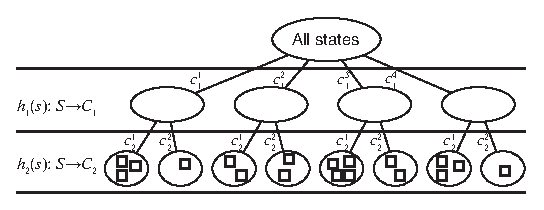
\includegraphics[width=3.2in]{chef/figures/cupa}
  \caption{\cupa state partitioning.  Each level corresponds to a state classification scheme.  Child nodes partition the parent node according to the classification at their level.}
  \label{fig:cupa}
\end{figure}
%
\cupa selects a new state for exploration by performing a random descent in the classification tree, starting from the root.  When reaching a leaf, the strategy takes out a random state from the state set and returns it to the symbolic execution engine for exploration.  By default, all sibling classes on each level have equal probability of being picked, but they can be assigned weights if required.

A \cupa strategy is parameterized by the number $N$ of levels in the tree and a classification function $h_i$ for each level $i=1 \ldots N$.  \chef uses two instantiations of \cupa: one optimized for covering high-level paths (Section~\ref{sec:chef:cupa-paths}) and one for covering the high-level CFG, i.e., statements (Section~\ref{sec:chef:cupa-coverage}).

\subsection{Path-optimized CUPA}
\label{sec:chef:cupa-paths}

A low-level strategy unaware of the high-level program would be implicitly biased towards picking high-level instructions that fork more low-level states than others, such as string operations or native calls.
%
To mitigate this, we instantiate a two-level \cupa strategy using the following classes:
\begin{enumerate}
\item The location of the state in the high-level symbolic execution tree.  This is the occurrence of the state's high-level program counter (\hlpc) in the unfolded high-level CFG, referred to as the dynamic \hlpc.  We choose the dynamic \hlpc to give each high-level path reaching the \hlpc the same chance to fork and subsequently diverge.
\item The low-level x86 program counter of the state.  This classification reduces the selection bias of ``hot spots'' of path explosion within a single complex instruction, such as a native function call.
\end{enumerate}

\subsection{Coverage-optimized CUPA}
\label{sec:chef:cupa-coverage}

Based on a coverage-optimized strategy introduced by the \klee symbolic execution engine~\cite{klee}, we developed a \cupa instance that partitions states according to their minimum distance to branches leading to uncovered code.
%
Alas, dynamic language interpreters do not generally have a static CFG view of the program, so code that has not been covered yet is not accessible to the search strategy.  The high-level CFG of the target program is dynamically discovered along each execution path.  On this CFG, we employ heuristics that (1) identify the instruction opcodes that may branch, and (2)~weigh the state selection toward states that are closer to these potential branching points.

First, \chef identifies the branching opcodes by collecting all high-level instructions that terminate a basic block with an out-degree in the CFG of at least $2$ (i.e., cause branching in the control flow).   We then eliminate the 10\% least frequent opcodes, which correspond to exceptions or other rare control-flow events.
%
Second, \chef identifies the potential branching points as those instructions in the CFG that have a branching opcode (as previously identified) but currently only one successor.
%
Finally, \chef computes for each execution state the distance in the CFG to the closest such potential branching point.

Having computed this information, we instantiate a two-level \cupa strategy with the following classes:
\begin{enumerate}
\item The static \hlpc of the state in the high-level CFG.  On this level, each class is weighted by $\frac{1}{d}$, where $d$ is the distance in the inferred high-level CFG to the closest potential branching point, making states at locations close to a target more likely to be selected.
\item The state itself (so each partition has a single element).  On this level, the states are weighted by their \textit{fork weight}.
\end{enumerate}

Fork weight is computed by counting the number of consecutive forks at the same low-level program counter (i.e., at an input-dependent loop in machine code).  States $1, \ldots, n$ forking from the same path at the same location get weights $p^n, p^{n-1}, \ldots, 1$, where $p < 1$ de-emphasizes states forked earlier ($p = 0.75$ in our implementation).  The last state to fork at a certain location thus gets maximum weight, because alternating the last decision in a loop is often the quickest way to reach different program behavior (e.g., to satisfy a string equality check).

%%% Local Variables: 
%%% mode: latex
%%% eval: (visual-line-mode)
%%% fill-column: 1000000
%%% TeX-master: "main"
%%% End:


\section{Packaging the Interpreter for Symbolic Execution}
\label{sec:chef:recipe}
Integrating an interpreter in \chef requires preparing a virtual machine that includes the interpreter binary, a symbolic test library, and a launcher.
%
To communicate with the interpreter runtime, \chef provides an API (Table~\ref{tab:chef:api}) that will be explained along with its use.

\begin{table}
\centering
\small
\begin{tabular}{| l | l | }
\hline
\textbf{API Call} & \textbf{Description} \\
\hline
\codebit{log\_pc(pc, opcode)} & Log the interpreter PC and opcode \\
\hline
\codebit{start\_symbolic()} & Start the symbolic execution \\
\codebit{end\_symbolic()} & Terminate the symbolic state \\
\hline
\codebit{make\_symbolic(buf)} & Make buffer symbolic \\
\codebit{concretize(buf)} & Concretize buffer of bytes \\
\codebit{upper\_bound(value)} & Get maximum value for expression on current path \\
\codebit{is\_symbolic(buf)} & Check if buffer is symbolic \\
\codebit{assume(expr)} & Assume constraint \\
\hline
\end{tabular}
\caption{The \chef API used by the interpreters running inside the S2E VM.}
\label{tab:chef:api}
\end{table}

\paragraph{Preparing the Interpreter Binary}

In principle, \chef can run unmodified interpreters for major popular languages, such as Python and JavaScript.
%
\chef automatically obtains from the running interpreter the stream of high-level program counters (HLPCs) for each execution path, required by the state adapter to reconstruct the high-level symbolic execution tree (Section~\ref{sec:chef:hlcf}).

In practice, however, applying a number of optimizations in the interpreter implementation significantly improve symbolic execution performance (Section~\ref{sec:chef:optimizeforsymbex}).


\paragraph{The Symbolic Test Library}

The unit of symbolic execution in \chef is the \emph{symbolic test}.
%
A symbolic test is a class, function, or other language-specific construct that encapsulates the symbolic input setup, the invocation, and the property checking of the feature targeted by the test.
%
A symbolic test is similar to a unit test, except for an extra set of primitives for creating symbolic values.

The symbolic tests are written in the same language as the target, and require runtime support in the form of a language-specific \emph{symbolic test library}.
%
The symbolic test library provides the developer interface for writing symbolic tests.
%
In addition, it translates the requests for marking language values as symbolic into the \chef API primitives for marking memory buffers as symbolic (the \codebit{make\_symbolic} call, together with the \codebit{assume} call for defining conditions over the input).
%
For example, when a symbolic test requests a 10-character symbolic string, the symbolic test library creates a concrete 10-character string object, then it finds its buffer address in the internal representation and marks the buffer as symbolic.
%
As a result, the symbolic test library is typically implemented as a native extension module, so it gains access to the internal data structures of the interpreter.

%% During symbolic execution, the low-level engine generates test cases as concrete assignments to the memory bytes marked as symbolic.
%% %
%% The \chef test library takes care of translating the concrete bytes back to string objects reported as test cases to the developer.

The execution of the interpreter in the virtual machine is bootstrapped by a launcher.  The launcher receives the location of the symbolic test (e.g., the module file and the class name, for Python) and runs the interpreter binary with the appropriate arguments such that it starts executing the symbolic test.
%
The launcher is typically a small web server running inside the guest, listening for commands from \chef.

%%%%%%%%%%%%%%%%%%%%%%%%%%%%%%%%%%%%%%%%%%%%%%%%%%%%%%%%%%%%%%%%%%%%%%%%%%%%%%%%

\subsection{Automated High-level Control Flow Detection in Interpreters}
\label{sec:chef:hlcf}

We defined a high-level path as a sequence of statements identified by high-level program counters (HLPCs).  In this section, we present the concrete semantics of the HLPC and how \chef obtains it automatically from a running interpreter.

\begin{figure}
  \centering
  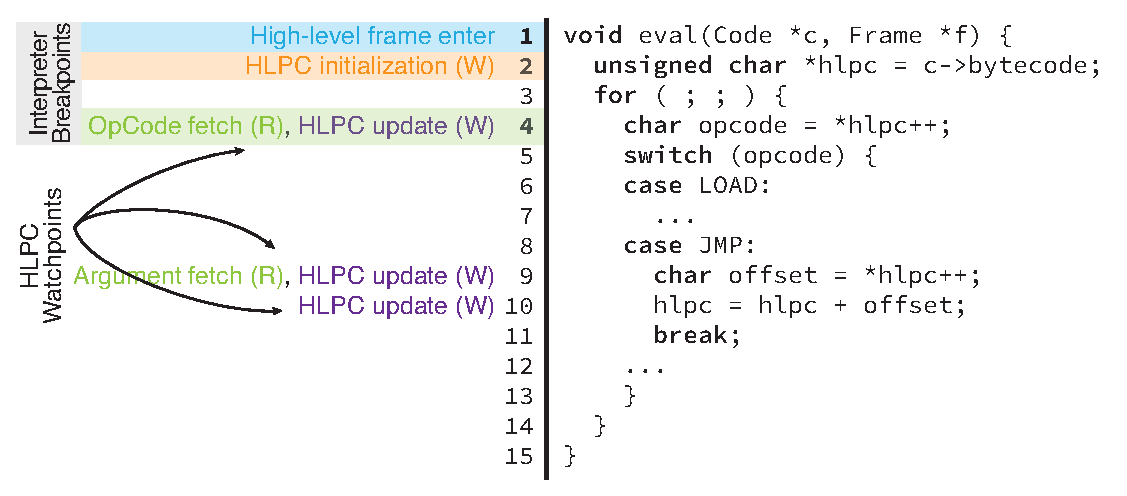
\includegraphics[width=0.8\textwidth]{chef/figures/interp-model}
  \caption{Structure of interpretation loop in most common interpreters.  Lines 1, 2, and 4 are three key HLPC points.  High-level control flow changes at Lines 4, 9, and 10 are detected at runtime by watchpoints on HLPC address identified at Line 2.}
  \label{fig:chef:interp-model}
\end{figure}

\paragraph{Standard Interpretation Model}

In general, obtaining the high-level program counter in a running interpreter is undecidable, because the boundaries between program statements are a high-level property of the language, and the separation may not reflect in the low-level implementation.
%
Even at the high level, statement boundaries may be ambiguous due to functional constructs, such as lambda functions and list comprehensions, or data definitions mixed with control flow, such as the class definitions in Python.

In practice, however, most interpreters follow a common structure that \emph{can be detected automatically}.
%
Instead of directly interpreting the source program, interpreters first compile it to an intermediate bytecode representation, which is interpreted instruction by instruction.  The bytecode is typically kept in per-function memory buffers.
%
When a function is called, the interpreter pushes a frame on its high-level stack, which contains a pointer variable to the next instruction in the function bytecode buffer.
%
An interpretation function receives the function bytecode and the stack frame, then executes the bytecode instructions one by one, while updating the HLPC variable of the frame (the right half of Figure~\ref{fig:chef:interp-model}).
%
We confirmed the generality of this approach by inspecting the source code of the most popular interpreters for Python, JavaScript (Mozilla's SpiderMonkey and WebKit's JavaScriptCore), Ruby, PHP, and Lua.

For these interpreters, we define the \chef high-level statements to be bytecode instructions, and their HLPC to be their address in the bytecode buffer.
%
As a result, to track the HLPC of the execution state, \chef monitors updates to the HLPC variable of the top high-level stack frame.

\paragraph{Tracking the HLPC Variable in the Interpreter}

To obtain the address of the top HLPC variable on the stack, \chef monitors three key locations in the interpretation function that summarize its HLPC update behavior:
%
(1) the address of the function itself, (2) the address of the statement that initializes the HLPC variable, and (3) the address of the statement that fetches the next opcode in the bytecode buffer.  The locations are highlighted on the left half of Figure~\ref{fig:chef:interp-model}.
%
\chef uses them as follows.

First, \chef maintains a stack of HLPC frames that track the interpreter's own high-level frames.
%
When the interpreter enters the interpretation function, \chef pushes a new HLPC frame on the current execution state.  A HLPC frame contains the address of the HLPC variable and its last value in the corresponding high-level frame of the interpreter.

Second, when the interpreter executes the HLPC initialization statement, \chef stores in the HLPC frame the memory address written to by the statement as the address of the HLPC variable.

Third, when the interpreter executes the opcode fetching statement, \chef marks the beginning of a new high-level statement at the address given by the current HLPC value.

During the execution of the interpretation function, \chef sets a watchpoint on the HLPC variable in the current frame.
%
When the variable is updated---e.g., when the next instruction is fetched, or after a branch or loop iteration---\chef correspondingly updates the HLPC value and the high-level symbolic execution tree, as needed.

\paragraph{Constructing the Interpreter HLPC Summary}

Before an interpreter is used for symbolic execution, \chef constructs its three-location HLPC summary.
%
The summary is constructed once for each interpreter binary.

First, \chef records all memory writes in the interpreter, when running a special developer-provided ``calibration'' script.
%
For each write, \chef records the interpreter location (x86 PC), the memory address, and the value written.

The role of the calibration script is to create HLPC update patterns that are recognizable among other memory writes.
%
The calibration script should run long enough that the HLPC patterns become clearly distinguishable.

To this end, \chef uses a linear sequence of instructions to create a linear HLPC update pattern.
%
We assume that the interpreter compiles a linear program (no branches) to a linear sequence of bytecode instructions.

After all memory writes are collected, \chef groups them by address and discards the groups whose values are not monotonically increasing.
%
Among the remaining groups, \chef discards those with fewer writes than the number of statements in the calibration program.  For this step, we assume that each statement corresponds to one or more bytecode instructions.
%
Finally, \chef discrads the groups whose write value deltas are larger than the size of a bytecode instruction.  We empirically determined an upper bound threshold of 1KB.

At the end, there should be exactly one remaining group, whose address refers to the HLPC variable of the frame of the recorded execution.

From the HLPC variable, \chef obtains the three-location summary.
%
The HLPC initialization location is the x86 PC of the first write operation in the remaining group.
%
The HLPC initialization location then leads to the address of the interpretation function, either by dynamically tracking the low-level program stack, or by using debug symbols in the interpreter binary.
%
Finally, the opcode fetch point corresponds to the first memory read of the HLPC variable, inside the interpretation function.

In case the calibration ends with no remaining memory write group, or more than one group remaining, the calibration fails.
%
This could happen, for instance, when the calibration is attempted on a non-conforming interpreter, or when the calibration script is too short.  To this end, we empirically determined that a 100-statement calibration script is sufficient for a successful calibration for all interpreters we tested.

In principle, defining program statements at an intermediate representation risks missing paths at the high-level.
%
This would happen, for instance, if the interpreter translated code with complex control flow to a linear bytecode sequence.
%
However, in our experience, we noticed that the translated bytecode follows closely the structure of the program.
%
In particular, interpreters perform little or no optimization on the bytecode.

\paragraph{Manually Annotating the High-level Program Counter}

When the interpreter structure diverges from our assumptions, \chef provides a fallback option of manually annotating the interpreter with the HLPC information.


%%%%%%%%%%%%%%%%%%%%%%%%%%%%%%%%%%%%%%%%%%%%%%%%%%%%%%%%%%%%%%%%%%%%%%%%%%%%%%%%

\subsection{Interpreter Optimizations}
\label{sec:chef:optimizeforsymbex}

In order to maximize performance, interpreters make heavy use of special cases and sophisticated data structures.  Unfortunately, these features hurt the performance of symbolic execution by amplifying path explosion and increasing the complexity of symbolic formulas~\cite{overify}.

We identify a number of optimizations that preserve the interpretation semantics but significantly improve symbolic execution performance.  The optimizations use the \chef API in the last block of rows in Table~\ref{tab:chef:api}.

\paragraph{Neutralizing Hash Functions}

Hash functions are especially common in interpreters, due to the internal use of hash tables for associative data structures (e.g., Python dictionaries or Lua tables).  However, they are generally a problem in symbolic execution: a symbolic value added to a hash table (a)~creates constraints that essentially ask the constraint solver to reverse a hash function, which is often hard, and (b)~causes the exploration to fork on each possible hash bucket the value could fall into.
%
A simple and effective optimization is to \emph{neutralize the hash function}, i.e., replace it with a degenerate one returning a single constant. This change honors the usual contracts for hash functions (equal objects have equal hashes) and will turn hash lookups into list traversals.

\paragraph{Avoiding Symbolic Pointers}

Input-dependent pointers (also referred to as symbolic pointers) may point to multiple locations in the program memory, so a pointer dereference operation would have to be resolved for each possible location.  In practice, symbolic execution engines deal with this situation in one of two ways:
%
(a)~fork the execution state for each possible concrete value the symbolic pointer can take; or
%
(b)~represent the dereference symbolically as a read operation from memory at a symbolic offset and let the constraint solver ``deal'' with it.
%
Both ways hurt symbolic execution, either by causing excessive path explosion or by burdening the constraint solver.

While there is no generic way to avoid symbolic pointers other than concretizing their values (the \codebit{concretize} API call) at the price of losing completeness, there are specific cases where they can be avoided.

First, \emph{the size of a buffer can be concretized} before allocation.  A symbolic size would most likely cause a symbolic pointer to be returned, since a memory allocator computes the location of a new block based on the requested size.  To avoid losing completeness, a symbolic execution-aware memory allocator can determine a (concrete) upper bound on the requested size and use that value for reserving space, while leaving the original size variable symbolic.  This way, memory accesses to the allocated block would not risk being out of bounds.  Figure~\ref{fig:sym-malloc} shows how the \chef API is used to wrap a call to the \codebit{malloc} function in the standard C library.

\begin{figure}
  \centering
  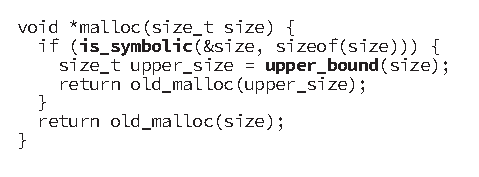
\includegraphics[width=2.6in]{chef/figures/mallocopt}
  \caption{Example of a symbolic execution-aware \codebit{malloc} function wrapper created using the \chef API.  If the allocation size is symbolic, the wrapper determines its upper bound and issues a concrete request to the underlying implementation.}
  \label{fig:sym-malloc}
\end{figure}

Second, \emph{caching and ``interning'' can be eliminated}.  Caching computed results and value interning (i.e., ensuring that a single copy of each possible value of a type is created) are common ways to improve the performance of interpreters.  Alas, when a particular value is computed, its location in memory becomes dependent on its value. If the value was already in the cache or in the interned store, it is returned from there, otherwise a new value is computed.  During symbolic execution, this logic becomes embedded in the value of the returned pointer, which becomes symbolic.  Disabling caching and interning may hurt the native performance of the program, but it can give a significant boost when running inside a symbolic execution engine.

\paragraph{Avoiding Fast Paths}

A common way to speed-up the native performance of a function is to handle different classes of inputs using faster specialized implementations (``fast paths'').  For example, a string comparison automatically returns false if the two strings have different lengths, without resorting to byte-wise comparison.

Fast paths may hurt symbolic execution because they cause symbolic branches in the code checking for the special input conditions.  \emph{Eliminating short-circuited returns} can reduce path explosion.  Instead of returning to the caller as soon as it produced an answer, the function continues running and stops on an input-independent condition.  For example, when comparing two strings of concrete length, a byte-wise string comparison would then traverse the entire string buffers in a single execution path, instead of returning after the first difference found.


%%% Local Variables: 
%%% mode: latex
%%% eval: (visual-line-mode)
%%% fill-column: 1000000
%%% TeX-master: "main"
%%% End:


\section{Summary}

Implementing and maintaining a symbolic execution engine is a significant engineering effort. It is particularly hard for interpreted dynamic languages, due to their rich semantics, rapid evolution, and lack of precise specifications.
%
\chef provides an engine platform that is instantiated with a language interpreter, which implicitly defines the complete language semantics, and results in a correct and theoretically complete symbolic execution engine for the language.
%
A language-agnostic strategy for selecting paths to explore in the interpreter allows the generated engine to systematically explore and test code in the target language effectively and efficiently.
%
\chef is available at {\urlstyle{same}\url{http://dslab.epfl.ch/proj/chef}}.


%%%%%%%%%%%%%%%%%%%%%%%%%%%%%%%%%%%%%%%%%%%%%%%%%%%%%%%%%%%%%%%%%%%%%%%%%%%%%%%%

\iffalse
\section{Symbolically Executing the Interpreter}

Building a correct and complete symbolic execution engine for an interpreted language is generally harder than building one for a low-level language. 
%
Statements of interpreted languages can wrap complex operations that, in lower-level languages, would be implemented through libraries. For instance, Python strings are a built-in type offering more than 30 operations (such as \codebit{find}) as part of the language, implemented natively in the interpreter. 
%
Other language features that allow to inspect or even modify the code itself, i.e., runtime reflection, are even more tedious to implement and very hard to get right.

Finally, besides requiring an enormous initial effort to build a symbolic execution engine that fully supports them, dynamic languages also evolve fast. This implies constant, labor-intensive maintenance and co-evolution of the symbolic execution engine, if it is to keep up with the newest versions of the language.

Considering the difficulty of directly supporting interpreted languages, we resort to symbolically executing the interpreter itself, since it completely defines the semantics of the target language as a function of the semantics of the language the interpreter is implemented in.
%
After compiling the interpreter to a format supported by an existing symbolic execution engine, one can symbolically execute an interpreted program by symbolically executing the interpreter with the target program as argument.
%
However, even though in principle this direct approach yields a symbolic execution engine for the target language, it is impractical, due to the engine not being aware of the control flow of the interpreted program.

\paragraph{High- vs. Low-level Program Paths}

\begin{figure}
  \centering
  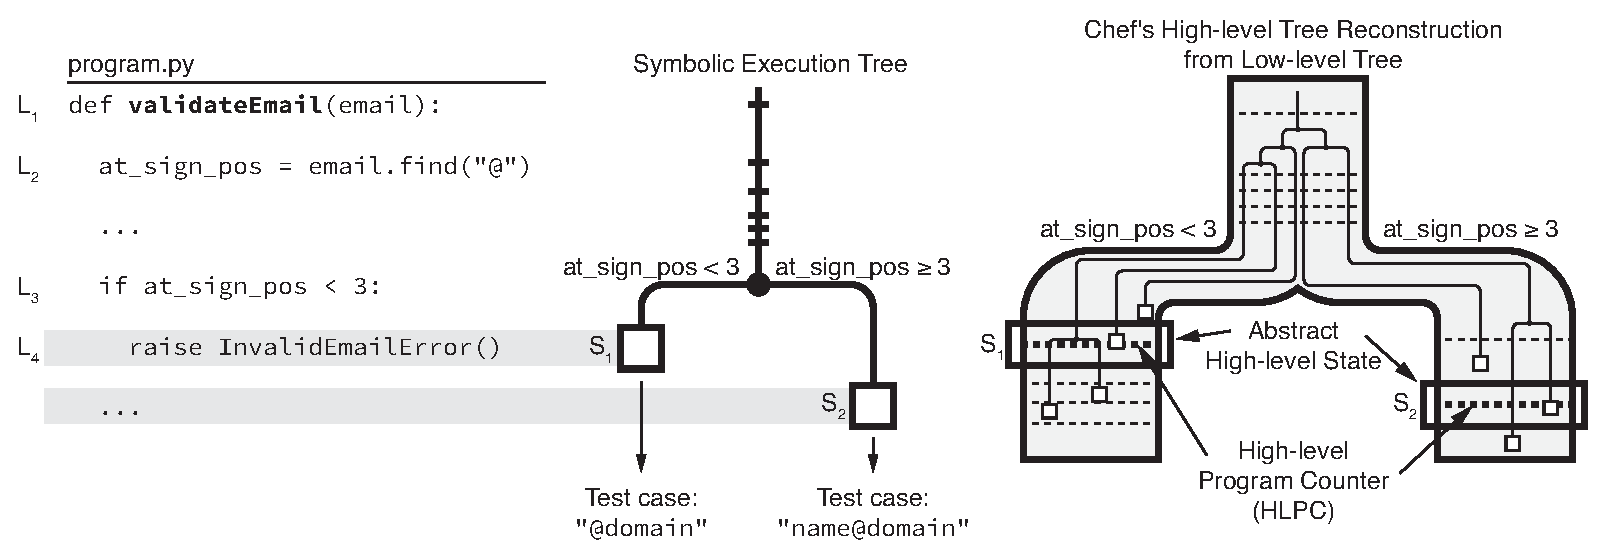
\includegraphics[width=2.2in]{chef/figures/running-example}
  \caption{Two examples of Python code that lead to path explosion when the interpreter running it is symbolically executed.}
  \label{fig:running-examples}
\end{figure}


An interpreted program conceptually executes both on a high level---the level of the target language---and a low level---the level of the interpreter.
%
A high-level program path is a sequence of values of the high-level program counter (\hlpc). Each \hlpc value corresponds to a program statement or bytecode instruction (both Python and Lua use intermediate bytecode).  Branches can occur explicitly at control flow statements, or implicitly through exceptions.
%
A low-level program path is a sequence of machine instructions from the interpreter binary, including its code for internal bookkeeping (e.g., details of reference counting and garbage collection).

Due to the additional implementation details, a single high-level path can map to multiple low-level paths.
%
Figure~\ref{fig:running-examples} shows two examples of Python code that have few high-level but many low-level paths. The \codebit{validateEmail} method has only two high-level paths, but its use of \codebit{string.find} leads to as many low-level paths as there can be characters in the \codebit{email} string.
%
The second example \codebit{average} may come as more of a surprise: even though it has just a single high-level path, symbolic execution can end up enumerating many low-level paths: Python uses arbitrary-precision integers, so the interpreter may have to iterate over digit vectors of arbitrary length, which can in principle spawn arbitrarily many paths.


\paragraph{Challenges for Search Strategies}
%
The search strategy of a low-level symbolic execution engine is oblivious to the high-level program structure of the target program, and it essentially just tries to cover the interpreter. This generally leads to covering the same high-level paths many times with multiple distinct low-level paths.
%
For instance, a high-level statement like \codebit{find} can lead to hundreds of alternate states, whereas a primitive integer comparison might just create a single one. Therefore, the low-level search strategy is likely to explore multiple ways for \codebit{find} to succeed or fail, without increasing high-level coverage, before eventually exploring the alternate outcome of the comparison.

\begin{figure}
  \centering
  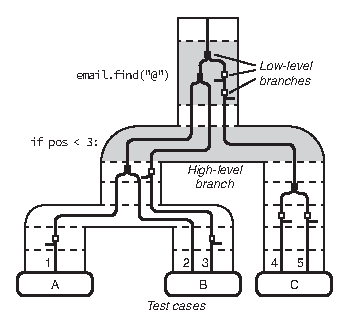
\includegraphics[width=2.8in]{chef/figures/hl-symbex}
  \caption{High-level execution tree (paths A, B, and C), as induced by its low-level execution paths (1--5) for the first running example in Figure~\ref{fig:running-examples}.  Dotted lines segment high-level execution paths into bytecode instructions.  One high-level path may correspond to multiple low-level paths explored.}
  \label{fig:hl-symbex}
\end{figure}

The key is to make the engine aware of the high-level interpreted program. By tracing the values of the \hlpc, the engine can construct a high-level control flow graph~(CFG) on the fly that can be be leveraged by the search strategy.

Alas, a strategy cannot straightforwardly determine future branching points in a high-level CFG: two low-level paths can fork from the same prefix \emph{before} their corresponding high-level paths do.  This can be due to having distinct bytecode instructions for comparisons and conditional jumps, or due to native library calls.  
%
In Figure~\ref{fig:hl-symbex}, three low-level paths fork within the single \hlpc location for \codebit{email.find}. The low-level paths remain on the same high-level path until reaching the branching \hlpc, where they diverge into two distinct high-level paths. The relevant alternate low-level states for covering the distinct high-level paths thus were located away from the location of the code interpreting the high-level control flow statement.
%
The issue of pre-determining branches is present also when exploring regular code, but it is ubiquitous when exploring code on interpreters.

\section{The \chef System}

We now present the architecture of \chef (Section~\ref{sec:chef:architecture}) and introduce CUPA, our state selection mechanism (Section~\ref{sec:chef:cupa}). We then describe CUPA optimized for exploring distinct high-level paths (Section~\ref{sec:chef:cupa-paths}) and optimized for high line coverage~(Section~\ref{sec:chef:cupa-coverage}).

\subsection{System Overview}
\label{sec:chef:architecture}

\chef is a platform for language-specific symbolic execution. Provided with an interpreter environment, which acts as an executable language specification, it becomes a symbolic execution engine for the target language (see Figure~\ref{fig:system-arch}).
%
The resulting engine can be used like a hand-written one, in particular for test case generation. When fed with a target program and a symbolic test case (also called test driver or test specification in the literature), it outputs a set of concrete test cases, as shown in Figure~\ref{fig:system-arch}.

\begin{figure}
  \centering
  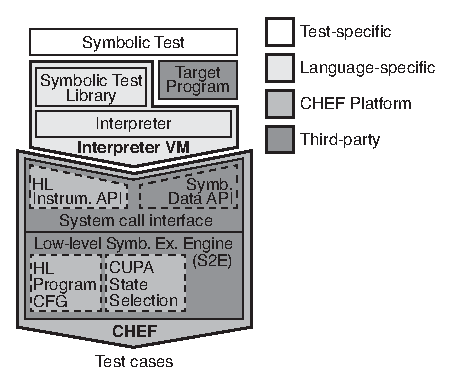
\includegraphics[width=2.6in]{chef/figures/system-arch}
  \caption{Schema of \chef's architecture.}
  \label{fig:system-arch}
\end{figure}

\chef is built on top of the S2E analysis platform~\cite{s2eSystem}. S2E symbolically executes a virtual machine containing the interpreter and a testing library at the level of machine code,  including the OS kernel, drivers, and user programs.  S2E provides an API that guest code can use to declare memory buffers as symbolic. Comparisons on symbolic values cause S2E to fork new paths, which are enqueued and explored following a search strategy.
%
\chef extends the S2E guest API with a high-level instruction instrumentation call (Section~\ref{sec:chef:exposehlpc}), invoked by interpreters to trace the currently executing high-level path.  The explored high-level paths are used to construct a high-level execution tree and a low-level to high-level mapping (i.e., the data structure shown in Figure~\ref{fig:hl-symbex}).  \chef uses a state selection strategy to maximize the ratio of high-level to low-level paths (Section~\ref{sec:chef:cupa}).
\fi

%%% Local Variables: 
%%% mode: latex
%%% eval: (visual-line-mode)
%%% fill-column: 1000000
%%% TeX-master: "main"
%%% End:


\chapter{Towards a Cloud Testing Service for PaaS}
\label{ch:paas}
In this chapter, we present our ongoing work on a cloud-based automated testing service for PaaS applications.
%
We first present the opportunities that computing clouds provide to developers, as well as the challenges developers face to test and secure their applications (Section~\ref{sec:paas:opportunity}).
%
We then give an overview of the usage of our PaaS-based testing service (Section~\ref{sec:paas:abstractions}).
%
The foundation of our service is a parallelization algorithm for symbolic execution that is the first to demonstrate linear scalability up to hundreds of cluster nodes (Section~\ref{sec:paas:parsymbex}).
%
On top, we introduce layered symbolic execution for addressing path explosion in systems composed of several stacked layers, such as protocol stacks (Section~\ref{sec:paas:layeredsymbex}).
%
Finally, we show how all pieces fit together in our S2E-based platform (Section~\ref{sec:paas:fedsymbex}).

\section{The Opportunity of the Cloud Application Model}
\label{sec:paas:opportunity}
Modern consumer software is increasingly relying on the ``cloud application'' model, where a browser- or mobile device-based client interacts with a functionally rich cloud service.
%
This model is prevalent in major systems like Facebook and GMail, as well as in smartphone and tablet ``apps'' like Instagram, Siri, or Dropbox.
%
For both developers and users, the economics are highly \mbox{attractive:} cloud-based applications offer ubiquitous access, transparent scaling, and easy deployment at low cost.

The hidden cost is that cloud apps introduce security, privacy, and availability risks. They store and process critical information remotely, so the impact of failures is higher in this model than for single-user desktop apps~\cite{web-failures-tr}.  This increases the importance of testing for cloud applications.

Rapid advances in development and deployment tools have significantly lowered the barrier to entry for developers, but these tools lack similarly advanced support for testing. Platform-as-a-service (PaaS) offerings, such as Google App Engine or Microsoft Azure, provide easy-to-use interfaces with automated deployment fully integrated into development environments.
%
However, testing tools for apps running on PaaS are still immature, test automation is limited, and developers are left with the laborious and error-prone task of manually writing large numbers of individual test cases.

Integration tests, which complement unit tests by checking that all the components of a fully deployed cloud application work together correctly, are especially tedious to write and set up in such an environment.
%
PaaS-based cloud applications typically use frameworks with a layered communication architecture and perform some processing at each of the layers. Writing a full integration test then requires to carefully craft an HTTP request that successfully passes through all application and framework layers and triggers the desired behavior, while being transformed from one representation to another at each step (e.g., from an HTTP request to JSON to language objects).

Spending precious developer time on testing for improving security and reliability is particularly unattractive in a viciously competitive environment.  Promoted by the ability to deploy virtually instantly and at low cost, the pressure is to use features to quickly acquire a large user base. Security and reliability testing is a long-term investment and does not pay off immediately, thus it is often deferred for later.
%
High-profile failures of cloud applications~\cite{bugs-linkedin,bugs-gmail} are thus likely to become a common occurrence, unless we can make testing easy and cheap.

We argue that {\em testing} must become at least as easy as {\em deploying} a new app. PaaS has made the latter easy, leaving the former just as hard to do as before.  A dedicated testing service must therefore become an integral component of PaaS.
%
Recent commercial test automation systems (CloudBees, Skytap, SOASTA, etc.) relieve developers of managing their own test infrastructure, but still require them to write test suites; we aim to further relieve developers of having to write individual tests.
%
Just as modern PaaS APIs spare developers from having to manage the building blocks of their applications, so should they spare developers from manually writing test cases, and instead offer means to automatically test apps based on only minimal input from developers.

The recent progress in automated test case generation and, in particular, symbolic execution takes an important step in this direction.  For a typical PaaS application like the example in Figure~\ref{fig:running-example}, a test case generator could use symbolic execution to automatically find HTTP packets that drive the execution to different parts of the code.
%
\begin{figure}
  \centering
  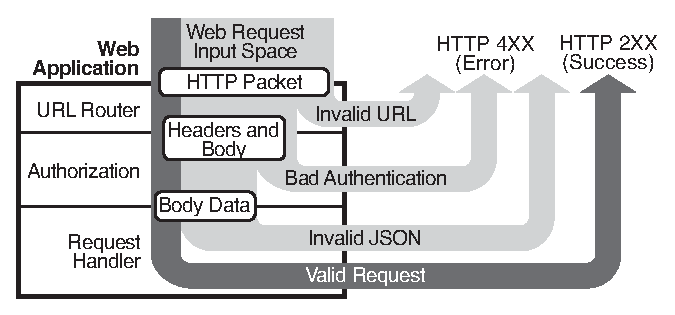
\includegraphics[width=0.7\textwidth]{paas/figures/web-flow}
  \caption{A sample cloud application.  Clients communicate with the server through web requests that traverse several layers inside the server before reaching the request handler logic.  From the total input space, most possible requests trigger errors in one of the processing layers (light arrows).  Only a small fraction of requests successfully traverses all layers and is handled inside the app (dark arrow).}
  \label{fig:running-example}
  \vspace{5pt}
\end{figure}
%
Unfortunately, these tools are challenging to apply to cloud apps: the number of execution paths successfully crossing all application layers is dwarfed by the vast number of possible error paths (dark vs.~light arrows in Figure~\ref{fig:running-example}).  Yet, most error paths are irrelevant to testing the high-level logic of the app itself (i.e., the innermost layer), because they test code that is part of the PaaS.

We introduce \textit{layered parameterized tests} (LPTs) for integration testing of PaaS-based cloud applications (Section~\ref{sec:paas:abstractions}). LPTs describe families of integration tests (in the spirit of parameterized unit tests~\cite{tillmann-puts}) across several application layers. We rely on developer-provided \textit{onion objects} to describe the layering of the data abstractions in the application; onion objects encode the multiple interpretations of input data as, e.g., an HTTP request, a JSON object, etc.

For the automatic generation of thorough test cases from LPTs, we introduce \emph{layered symbolic execution} (LSE), an automated program analysis that is tailored for the layered structure of cloud applications (Section~\ref{sec:paas:layeredsymbex}).

Symbolic execution is a resource-intensive task, so we horizontally scale it in the cloud by introducing the first symbolic execution parallelization algorithm to demonstrate linear scalability in the number of nodes (Section~\ref{sec:paas:parsymbex}).

Finally, we present a design and early prototype for a PaaS-integrated parallel testing service based on LSE~(Section~\ref{sec:paas:fedsymbex}).

%%% Local Variables: 
%%% mode: latex
%%% eval: (visual-line-mode)
%%% fill-column: 1000000
%%% TeX-master: "main"
%%% End:


\section{A PaaS Test Interface}
\label{sec:paas:abstractions}
We introduce an automated testing service integrated in PaaS.
%
Developers write layered parameterized tests (LPTs) and upload them with the cloud application to be executed by the test service.  The service uses LPTs to automatically generate application inputs (e.g., web requests and persistent data) that exercise the application layers of interest.  The developer writes LPTs by specifying the structure of the application inputs and a target property to be checked.

\paragraph{Developer Workflow}

\begin{figure}
  \centering
  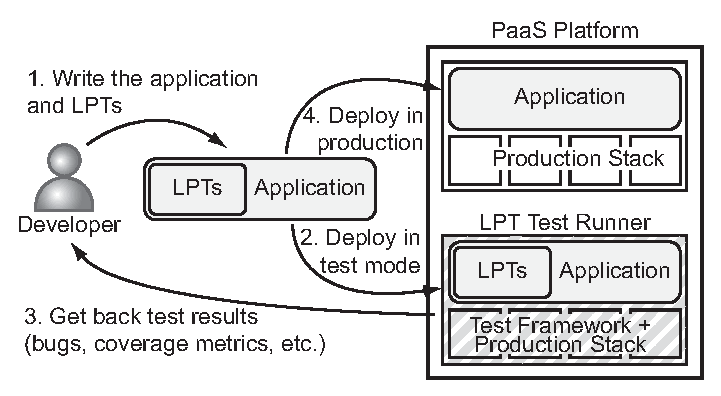
\includegraphics[width=0.8\textwidth]{paas/figures/developer-flow}
  \caption{Development flow for using a PaaS-integrated testing
    service.}
  \label{fig:development-flow}
\end{figure}

Figure~\ref{fig:development-flow} illustrates the workflow of a developer using our testing service.
%
The developer writes layered parameterized tests using a platform-provided testing API (step 1). She then deploys the app in test mode, which invokes the LPT test runner of the PaaS (step 2). This test runner is responsible for generating and running the individual test cases from the LPT, and it returns test results back to the developer (step 3). The develop-deploy-test cycle continues until the code is ready to be deployed in production (step 4).

% Might be misleading - the onion tests are much more powerful
% , and existing xUnit tests can be converted to onion tests.

%---------------------------------------------------------------------------
\paragraph{Layered Parameterized Tests}

An LPT specifies a family of executions (or, equivalently, classes of inputs) plus a set of properties (expressed as assertions) that are expected to hold for all these executions.
%
The specified family of executions can be large or even infinite; still, the test runner can often efficiently check whether the property is guaranteed to hold for the entire family (we give more details on the symbolic execution-based mechanism in Section~\ref{sec:paas:layeredsymbex}).  A traditional unit test can be seen as a special case of an LPT for which the input is fixed and any provided assertions are checked on a single execution only.

\begin{figure}
  \centering
  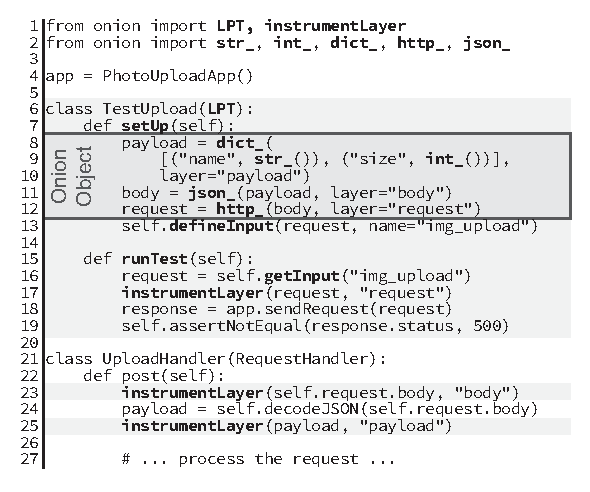
\includegraphics[width=0.7\textwidth]{paas/figures/overlay}
  \caption[An LPT example in Python for a photo management application.]{An LPT example in Python for a photo management application.  Highlighted code is the test code written by developers.  Names in bold denote the LPT-specific API added to the standard Python unit test framework.}
  \label{fig:test-lpt}
\end{figure}

\looseness=-1 LPTs are defined by developers using a platform-provided API in the implementation language of the application (e.g., Python).  The testing API builds on the popular xUnit testing paradigm~\cite{xunit} and extends it with constructs to specify the structure of families of application inputs.  The API is easily integrated with existing testing fixtures and frameworks that developers use today.

We illustrate the structure of an LPT and how it is used by the test runner using the example LPT \codebit{TestUpload} shown in Figure~\ref{fig:test-lpt}, which tests the upload functionality of a photo management application.  Under the \codebit{/upload} URL, the application accepts POST requests containing a JSON-encoded dictionary describing photo information.  Figure~\ref{fig:http-packet} shows an example HTTP request for the application.

We assume that the app follows the structure given in Figure~\ref{fig:running-example}, that it is written in Python using a popular web framework like Django~\cite{py-django} or WebApp~\cite{webapp2}, and that it is deployed on a PaaS infrastructure like Google App Engine~\cite{google-gae} or Heroku~\cite{heroku}.  The web framework takes care of dispatching any POST request to the \codebit{/upload} application URL to the \codebit{post} method of the \codebit{UploadHandler} class (lines 21--27).
%
The \codebit{TestUpload} LPT checks that, for arbitrary upload requests, the server never returns an internal error (HTTP 500) in its response.

\begin{figure}
  \centering
  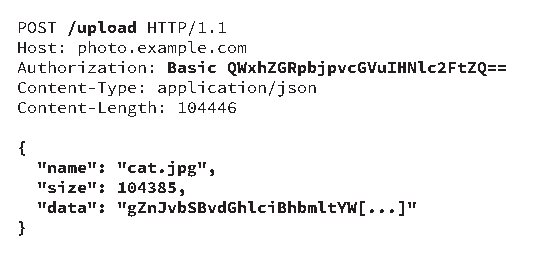
\includegraphics[width=0.7\textwidth]{paas/figures/http-packet}
  \caption[An example HTTP request for the upload feature of a photo management application.]{An example HTTP request for the upload feature of the photo management application.  The text in bold denotes input processed by the application at various layers.}
  \label{fig:http-packet}
\end{figure}

The test runner uses the LPT to automatically generate application
input according to the following procedure:

\begin{enumerate}
% Step 1
\item The test runner invokes the \codebit{setUp} method (line~7),
  which declares the application inputs and their structure as
  \emph{onion objects} (described below) using the
  \codebit{defineInput} call at line~13.
% Step 2
\item Based on the onion objects, the test runner generates a default
  input for the application.
% Step 3
\item The test runner invokes \codebit{runTest}, which retrieves the
  concrete input generated by the test runner with a call to
  \codebit{getInput} (line~16).  In our example, the input is a web
  request, which is then sent to the application (line~18).  Behind
  the scenes, the web framework dispatches the request to the
  \codebit{post} method of \codebit{UploadHandler} (line~22).  When
  the handler finishes handling the request, a response object with a
  status code and body is returned.  In our example, the LPT checks
  that no internal error (HTTP 500) occurred during request handling
  (line~19).
% Step 4
\item Based on the information collected during the execution of
  \codebit{runTest} (described below), the test runner uses the onion
  objects to generate a new application input (available to the LPT
  through the \codebit{getInput} call) and goes back to step 3 for a
  new iteration.  
%
  Any assertion failures triggered by the generated inputs are
  reported to the developers.
\end{enumerate}
%
Note that the generation and execution of multiple inputs is well
suited for parallelization across multiple nodes in the cloud. This
allows to leverage the availability of additional nodes to reduce the
total testing time.

The test runner uses symbolic execution to generate new inputs (described in more detail in Section~\ref{sec:paas:layeredsymbex}). To generate inputs that exercise the application at specific layers, the test runner needs:
\begin{itemize}
\item the unwrapped application inputs for the current execution at the different application layers, provided by developers through annotations in the application source code; and
\item information about the input structure, provided by the LPT's onion objects.
\end{itemize}

\paragraph{Annotating Application Layers}

A web request traverses several processing layers in an application.  First, it is received as an HTTP packet string; second, it is decoded into a URL, a set of headers, and request a body; third, the body contents is decoded and processed. Depending on the application framework, processing can involve additional layers, e.g., for converting JSON representations to language objects.

The application layers process data at corresponding layers of the input data (the bold parts of the HTTP request in Figure~\ref{fig:http-packet}). For instance, the application typically maps the URL to a request handler, checks the headers for authentication information, and processes the body contents in the request handler code.

To expose the application input to the LPT as it is being processed at each layer, developers annotate the variables holding the input data structures in the application source code.  Three layers have been declared in Figure~\ref{fig:test-lpt}: the HTTP request at line~17, the request body at line~23, and the JSON payload extracted from the body at line~25.  The \codebit{instrumentLayer} call attaches a layer name to a variable. Similar to assertion statements, the call is active when executed as part of a test invocation, but disabled in production, where the LPTs are not used.  For a typical web stack, only about three layers have to be annotated for each request handler, keeping the required effort on the developer side low.


%---------------------------------------------------------------------------
\paragraph{Onion Objects}

An \emph{onion object} is a data structure that describes the representations of the application input as it traverses multiple processing layers.  The onion object (i) enables more convenient assertion-writing by directly exposing the data layers, and (ii) enables automated test generation to focus on specific layers of the application. Onion objects are needed to specify the application inputs for onion tests, but they can also be used to store output as the cloud application constructs a response in layers.

The framed area in Figure~\ref{fig:test-lpt} shows the onion object for our running example.  The structure consists of a set of \emph{onion nodes} (the identifiers ending in an underscore) connected in a nested structure.  There is one onion node for each layer and one for each input structure or value that is supposed to be generated automatically by the test engine.  The abstraction level is declared using the \codebit{layer} parameter passed to the node constructor and matches one of the layers annotated in the code.  Structures and values can be nested within the same layer.  For example, the dictionary structure on lines~8--10 has constant keys and wildcard values of type \codebit{str\_} and \codebit{int\_}, which mimic the standard string and integer types.

\paragraph{Checking Properties}

LPTs express application properties through standard xUnit assertion statements (line~19 in the example).  Through the dynamic test generation mechanism explained in Section~\ref{sec:paas:layeredsymbex}, the test runner actively attempts to generate inputs that cause an assertion to be violated. Each generated test input not failing the assertion serves as a witness for an entire equivalence class of inputs that cannot violate the assertion.
%
When an assertion does fail, the input that caused the failure is reported back to the developer.

To allow input variables at each layer to be used in assertions, each onion node offers a \codebit{value} property that refers to the value matched in the current test execution (not shown in the example).

%%% Local Variables: 
%%% mode: latex
%%% eval: (visual-line-mode)
%%% fill-column: 1000000
%%% TeX-master: "main"
%%% End:


\section{Parallel Symbolic Execution in Cloud9}
\label{sec:paas:parsymbex}

Since the size of the execution tree is exponential in the number of branches, and the complexity of constraints increases as the tree deepens, state-of-the-art SEEs can quickly bottleneck on CPU and memory even for programs with just a couple \kloc.  We therefore build a parallel SEE that runs on a commodity cluster and enables ``throwing hardware at the problem.''

The key design goal is to enable individual cluster nodes to explore the execution tree independently of each other.  One way of doing this is to statically split the execution tree and farm off subtrees to worker nodes.  Alas, the contents and shape of the execution tree are not known until the tree is actually explored, and finding a balanced partition (i.e., one that will keep all workers busy) of an unexpanded execution tree is undecidable.  Besides subtree size, the amount of  memory and CPU required to explore a subtree is also undecidable, yet must be taken into account when partitioning the tree. Since the methods used so far in parallel model checkers~\cite{swarm,spin:multicore-modelchecking} rely on static partitioning of a finite state space, they cannot be directly applied to the present problem. Instead, \cnine partitions the execution tree {\em dynamically}, as the tree is being explored. 

%--------------------------------------------------
\paragraph{Dynamic Distributed Exploration}

\cnine consists of wor\-ker nodes and a load balancer (LB).  Workers run independent SEEs, based on \klee~\cite{klee}.  They explore portions of the execution tree and send statistics on their progress to the LB, which in turn instructs, whenever necessary, pairs of workers to balance each other's work load.  Encoding and transfer of work is handled directly between workers, thus taking the load balancer off the critical path.

The goal is to dynamically partition the execution tree such that the parts are {\em disjoint} (to avoid redundant work) and together they {\em cover} the global execution tree (for exploration to be complete).  We aim to minimize the number of work transfers and associated communication overhead.  A fortuitous side effect of dynamic partitioning is the transparent handling of fluctuations in resource quality, availability, and cost, which are inherent to large clusters in cloud settings.

\cnine operates roughly as follows: The first component to come up is the load balancer.  When the first worker node $W_1$ joins the \cnine cluster, it connects to the LB and receives a ``seed'' job to explore the entire execution tree.  When the second worker $W_2$ joins and contacts the LB, it is instructed to balance $W_1$'s load, which causes $W_1$ to break off some of its unexplored subtrees and send them to $W_2$ in the form of {\em jobs}.  As new workers join, the LB has them balance the load of existing workers.  The workers regularly send to the LB status updates on their load in terms of exploration jobs, along with current progress in terms of code coverage, encoded as a bit vector.  Based on workers' load, the LB can issue job transfer requests to pairs of workers in the form $\langle$~source worker, destination worker, \# of jobs~$\rangle$.  The source node decides which particular jobs to transfer.

\subsection{Worker-level Operation}
\label{sec:workerView}

A worker's visibility is limited to the subtree it is exploring locally.  As $W_i$ explores and reveals the content of its local subtree, it has no knowledge of what $W_j$'s ($i\ne j$) subtree looks like.  No element in the system---not even the load balancer---maintains a global execution tree.  Disjointness and completeness 
of the exploration (see Fig.~\ref{fig:architecture}) are ensured by the load balancing algorithm.

\begin{figure}[h!]
  \centering
  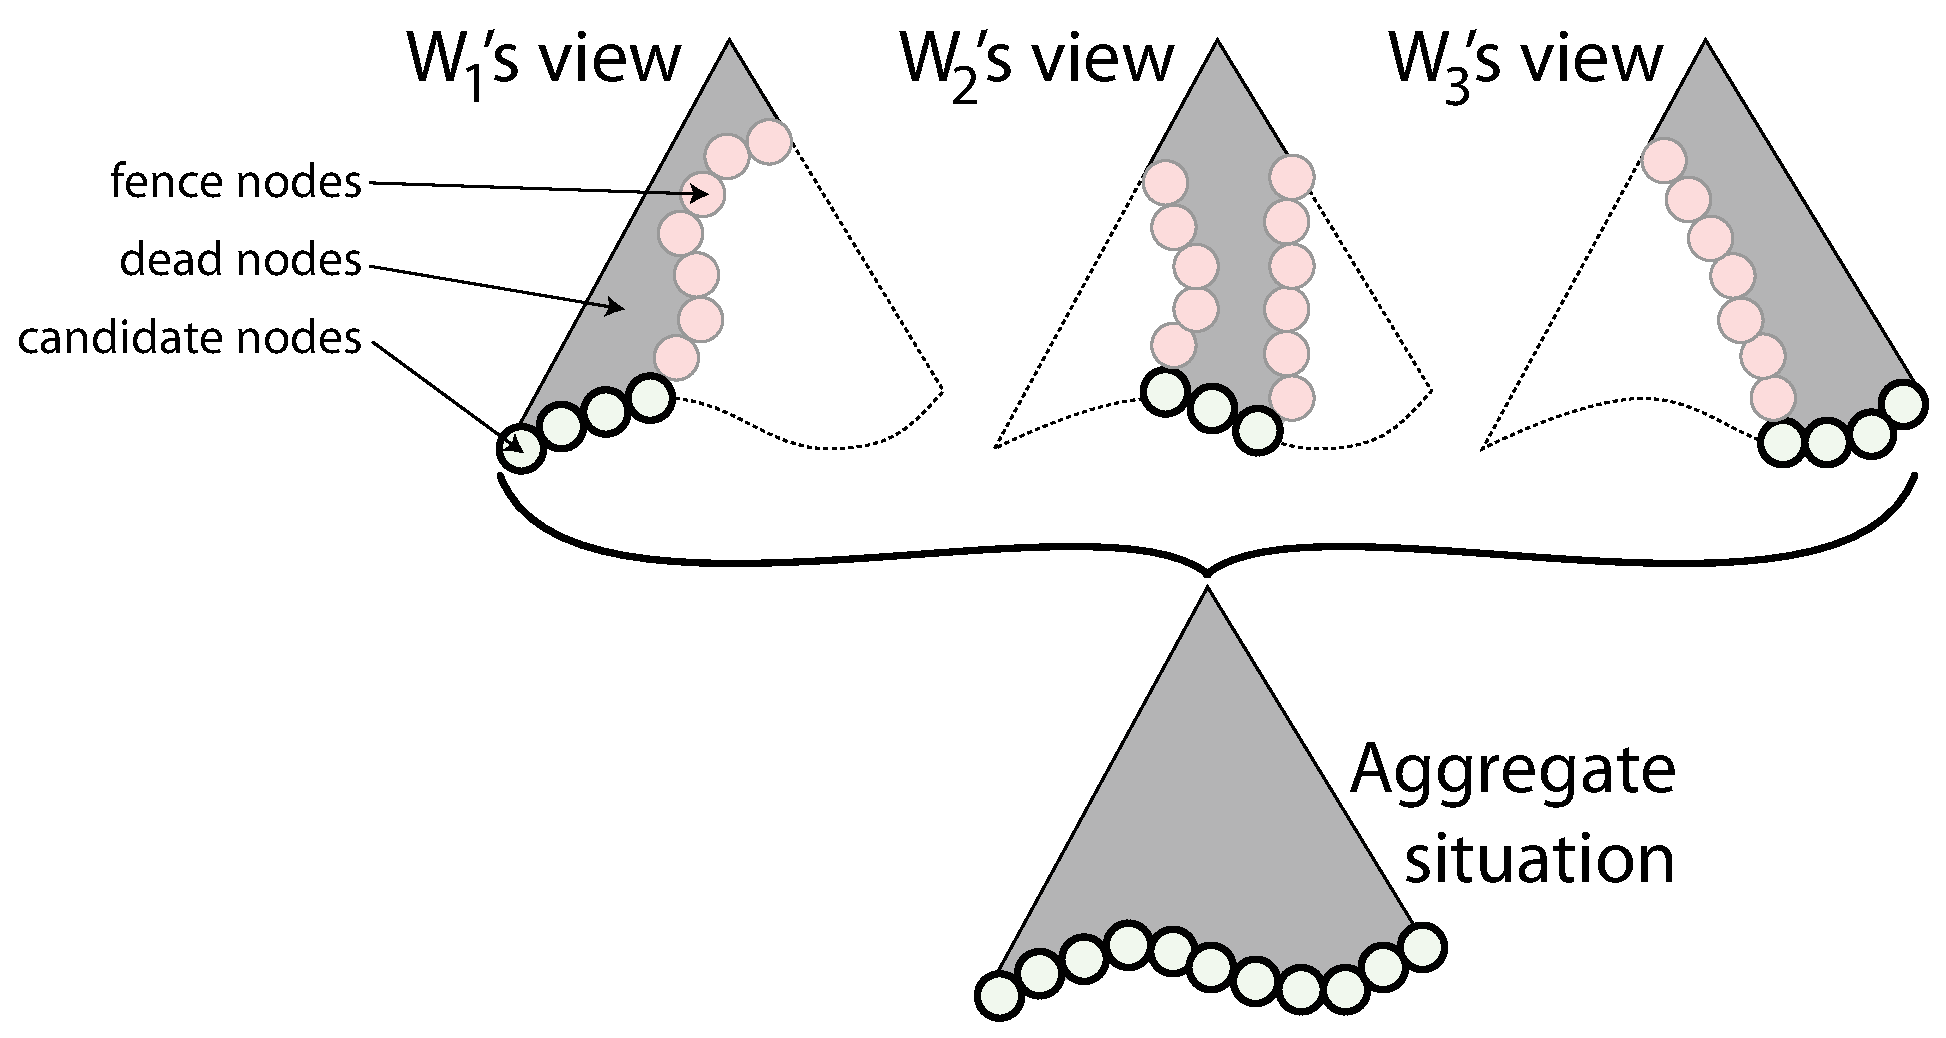
\epsfig{file=paas/figures/architecture-parsymbex, height=1.7in}
  \caption{Dynamic partitioning of exploration in \cnine.}
 \label{fig:architecture}
\end{figure}

\newcommand{\dead}{dead\xspace}
\newcommand{\fence}{fence\xspace}
\newcommand{\candidate}{candidate\xspace}
\newcommand{\virtual}{virtual\xspace}
\newcommand{\materialized}{materialized\xspace}

As will be explained later, each worker has the root of the global execution tree.  The tree portion explored thus far on a worker consists of three kinds of nodes: (1) internal nodes that have already been explored and are thus no longer of interest---we call them {\em \dead} nodes; (2) {\em \fence} nodes that demarcate the portion being explored, separating the domains of different workers; and (3) {\em \candidate} nodes, which are nodes ready to be explored.  A worker exclusively explores \candidate nodes; it never expands \fence or \dead nodes.

Candidate nodes are leaves of the local tree, and they form the \emph{exploration frontier}.  The work transfer algorithm ensures that frontiers are disjoint between workers, thus ensuring that no worker duplicates the exploration done by another worker.  At the same time, the union of all frontiers in the system corresponds to the frontier of the global execution tree. The goal of a worker  $W_i$ at every step is to choose the next \candidate node to explore and, when a bug is encountered, to compute the inputs, thread schedule, and system call returns that would take the program to that bug.

%--------------------------------------------------
\paragraph{Worker-to-Worker Job Transfer}
\label{sec:workTransfer}

\newcommand{\wsrc}{\ensuremath{W_s}\xspace}
\newcommand{\wdst}{\ensuremath{W_d}\xspace}

When the global exploration frontier becomes poorly balanced across workers, the load balancer chooses a loaded worker \wsrc and a less loaded worker \wdst  and instructs them to balance load by sending $n$ jobs from \wsrc to \wdst.  In the extreme, \wdst is a new worker or one that is done exploring its subtree and has zero jobs left.  

\wsrc chooses $n$ of its \candidate nodes and packages them up for transfer to \wdst.  Since a \candidate node sent to another worker is now on the boundary between the work done by \wsrc and the work done by \wdst, it becomes a \fence node at the sender.  This conversion prevents redundant work.

A job can be sent in at least two ways: (1) serialize the content of the chosen node and send it to \wdst, or (2) send to \wdst the path from the tree root to the node, and rely on \wdst to ``replay'' that path and obtain the contents of the node.  Choosing one vs. the other is a trade-off between time to encode/decode and network bandwidth: option (1) requires little work to decode, but consumes bandwidth (the state of a real program is typically at least several megabytes), while encoding a job as a path requires replay on \wdst.  We assume that large commodity clusters have abundant CPU but meager bisection bandwidth,
so in \cnine we chose to encode jobs as the path from the root to the \candidate node.  As an optimization, we exploit common path prefixes: jobs are not encoded separately, but rather the corresponding paths are aggregated into a job tree and sent as such.

\begin{wrapfigure}{r}{1in}
\vspace{-5mm}
%
%\includegraphics[height=50mm]{new-diagrams/worker-tree-thumb}
\hspace{-10mm}\includegraphics[height=50mm]{paas/figures/worker-tree-thumb}
%\caption{Example of a local worker tree.}
\vspace{-8mm}
\end{wrapfigure}

When the job tree arrives at \wdst, it is imported into \wdst's own subtree, and the leaves of the job tree become part of \wdst's frontier (at the time of arrival, these nodes may lie ``ahead'' of \wdst's frontier).  \wdst keeps the nodes in the incoming jobs as {\em \virtual} nodes, as opposed to {\em \materialized} nodes that reside in the local subtree, and replays paths only lazily.  A \materialized node is one that contains the corresponding program state, whereas a \virtual node is an ``empty shell'' without corresponding program state.  In the common case, the frontier of a worker's local subtree contains a mix of \materialized and \virtual nodes, as shown in the diagram above.

As mentioned earlier, a worker must choose at each step which \candidate node to explore next---this choice is guided by a {\em strategy}.  Since the set of \candidate nodes now contains both \materialized and \virtual nodes, it is possible for the strategy to choose a \virtual node as the next one to explore.  When this happens, the corresponding path in the job tree is replayed (i.e., the symbolic execution engine executes that path); at the end of this replay, all nodes along the path are \dead, except the leaf node, which has converted from \virtual to \materialized and is now ready to be explored.  Note that, while exploring the chosen job path, each branch produces child program states; any such state that is not part of the path is marked as a \fence node, because it represents a node that is being explored elsewhere, so \wdst should not pursue it.

\paragraph{Summary}

\newcommand{\status}{\ensuremath{\mathrm{status}}\xspace}
\newcommand{\alive}{\ensuremath{\mathrm{life}}\xspace}

A node $N$ in $W_i$'s subtree has two attributes, $N^{\status} \in$\{\materialized, \virtual\!\} and $N^{\alive} \in$\{\candidate, \fence, \dead\!\}.  A worker's frontier $F_i$ is the set of all \candidate nodes on worker $W_i$.  The worker can only explore nodes in $F_i$, i.e., \dead nodes are off-limits and so are \fence nodes, except if a \fence node needs to be explored during the replay of a job path.  The union $\cup F_i$ equals the frontier of the global execution tree, ensuring that the aggregation of worker-level explorations is complete.  The intersection $\cap F_i = \emptyset$, thus avoiding redundancy by ensuring that workers explore disjoint subtrees.  Fig.~\ref{fig:transitions} summarizes the life cycle of a node.

\begin{figure}[h!]
  \centering
  \hspace{-4mm}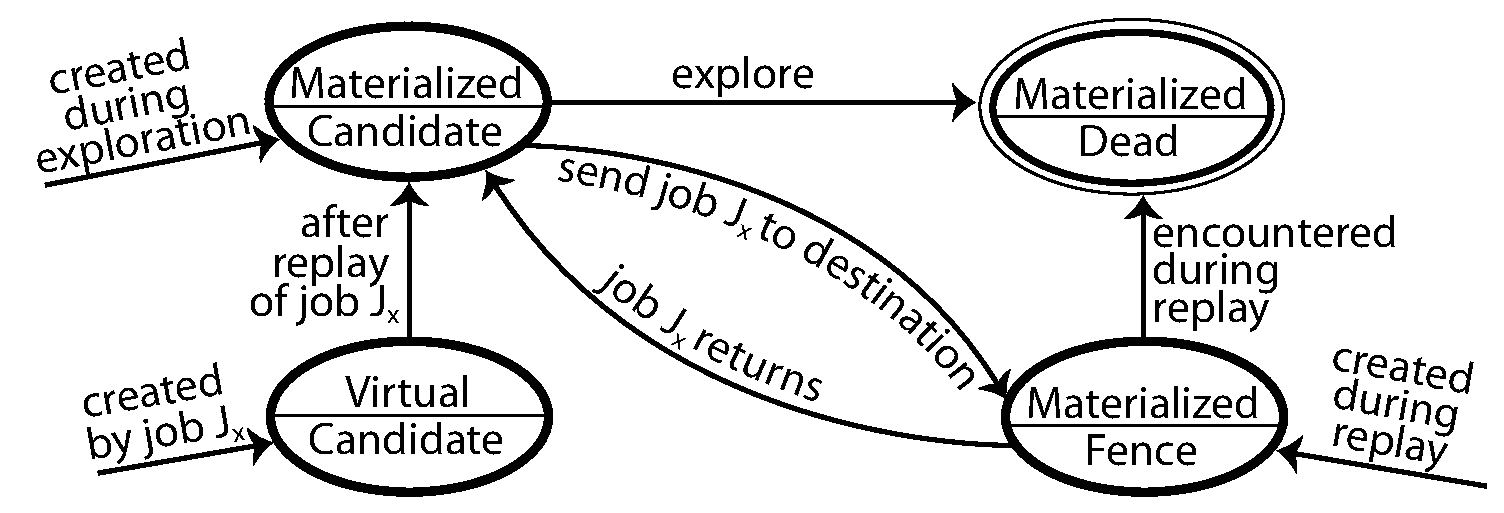
\epsfig{file=paas/figures/node-transitions, width=3.4in}
  \caption{Transition diagram for nodes in a worker's subtree.}
 \label{fig:transitions}
\end{figure}

As suggested in Fig.~\ref{fig:transitions}, once a tree node is \dead, it has reached a terminal state; therefore, a dead node's state can be safely discarded from memory.  This enables workers to maintain program states only for \candidate and \fence nodes.

%%%%%%%%%%%%%%%%%%%%%%%%%%%%%%%%%%%%%%%%%%%%%%%%%%%%%%%%%%%%%%%%%%%%%%%%%%%%%%%%

\subsection{Cluster-level Operation}
\label{sec:loadBalancing}

\paragraph{Load Balancing}

When jobs arrive at \wdst, they are placed conceptually in a queue; the \emph{length} of this queue is sent to the load balancer periodically.  The LB ensures that the worker queue lengths stay within the same order of magnitude.  The balancing algorithm takes as input the lengths $l_i$ of each worker $W_i$'s queue $Q_i$.  It computes the average $\bar{l}$ and standard deviation $\sigma$ of the $l_i$ values and then classifies each $W_i$ as underloaded ($l_i < max \{ \bar{l}-\delta \cdot \sigma, 0 \}$), overloaded ($l_i > \bar{l} + \delta \cdot \sigma$), or OK otherwise; $\delta$ is a constant factor.  The $W_i$ are then sorted according to their queue length $l_i$ and placed in a list.  LB then matches underloaded workers from the beginning of the list with overloaded workers from the end of the list.  For each pair $\langle W_i,W_j \rangle$, with $l_i < l_j$, the load balancer sends a job transfer request to the workers to  move $(l_j - l_i)/2$ \candidate nodes from $W_j$ to $W_i$.


%===========================================================================
\paragraph{Coordinating Worker-level Explorations}
\label{sec:globalStrategy}

Classic symbolic execution relies on heuristics to choose which state on the frontier to explore first, so as to efficiently reach the chosen test goal (code coverage, finding a particular type of bug, etc.). In a distributed setting, local heuristics must be coordinated across workers to achieve the global goal, while keeping communication overhead at a minimum. What we have described so far ensures that eventually all paths in the execution tree are explored, but it provides no aid in focusing on the paths desired by the global strategy.  In this sense, what we described above is a \emph{mechanism}, while the exploration strategies represent the \emph{policies}.

Global strategies are implemented in \cnine using its interface for building {\em overlays} on the execution tree structure.  We used this interface to implement distributed versions of all strategies that come with \klee~\cite{klee}; the interface is also available to \cnine users.  Due to space limitations, we do not describe the strategy interface further, but provide below an example of how a global strategy is built.

A coverage-optimized strategy drives exploration so as to maximize coverage~\cite{klee}.  In \cnine, coverage is represented as a bit vector, with one bit for every line of code; a set bit indicates that a line is covered.  Every time a worker explores a program state, it sets the corresponding bits locally. The current version of the bit vector is piggybacked on the status updates sent to the load balancer.  The LB maintains the current global coverage vector and, when it receives an updated coverage bit vector, {\small OR}s it into the current global coverage.  The result is then sent back to the worker, which in turn {\small OR}s this global bit vector into its own, in order to enable its local exploration strategy to make choices consistent with the global goal.  The coverage bit vector is an example of a \cnine overlay data structure.

%%% Local Variables: 
%%% mode: latex
%%% eval: (visual-line-mode)
%%% fill-column: 1000000
%%% TeX-master: "main"
%%% End:


\section{Layered Symbolic Execution}
\label{sec:paas:layeredsymbex}
In this section, we introduce \emph{layered symbolic execution} (LSE), an LPT execution technique that focuses on covering a particular application layer.  LSE uses symbolic execution---a test case generation technique that observes the program structure---to generate inputs in the representation of the layer of interest (e.g., HTTP headers or a JSON payload).  Each generated layer-level input is then assembled back into application-level input based on the structure encoded in the onion object, in order to form an integration test case.

Na\"ive application of dynamic test generation to execute the LPT for a cloud app is of little use: First, the path exploration can end up exploring many different paths within the framework code, but might test only a single path within the application layer over and over again. Second, the path conditions will encode many branches due to the multiple layers of parsing logic, making symbolic execution of cloud apps prohibitively expensive. Third, if the exploration is unaware of the connections between abstraction layers, blindly negating just single branch conditions will produce many infeasible paths before finding a new valid test input.

\paragraph{LSE and Onion Objects}

LSE relies on onion objects to mark input variables as symbolic and generate new values based on the alternate path conditions.  To this end, each onion object exposes a number of operations:

\begin{itemize}
\item \codebit{instrument(var)} instruments the variable \codebit{var}
  for symbolic execution, i.e., injects a fresh symbolic input value
  in dynamic test generation.  The variable is expected to match the
  structure described by the onion object.
%
\item \codebit{reconstruct(var, val)} applies an assignment of value \codebit{val} to variable \codebit{var} that is demanded by the satisfying assignment representing a new path. In doing the assignment, the function performs the necessary modifications to other variables to respect the cross-layer invariants.
%
\item \codebit{getDefault()} returns a default value for the object node. It is used for generating the initial test case or any padding values required by invariants (e.g., changing the content length field of an HTTP request requires to extend the actual contents).
\end{itemize}

For example, applying the \codebit{instrument} method of a string onion object on a string variable in Python marks as symbolic the string length and the contents of the character buffer.  Then, during symbolic execution, the alternate path constraint yields new values for the length and for the buffer.  The \codebit{reconstruct} method takes both values and creates a new Python string object.

The reconstruction method is essential for enforcing the object and cross-layer invariants of the input structure.  For instance, the length of the reconstructed string would always match the size of its buffer (and avoid spurious overflows); the Content-length HTTP header would always match the size of the new request body, and so on.

\paragraph{LSE Algorithm}

LSE allows the test runner to focus on exploring paths inside inner application layers. Conceptually, LSE decouples the input layers to give the test runner the flexibility to freely explore an individual layer. When constructing a new application input, LSE reconnects the layers, taking care to respect cross-layer invariants (e.g., the value of a JSON field has to be present also in the HTTP packet).
%
The LSE algorithm proceeds along the following steps:
\begin{enumerate}
\item Generate an initial valid input (i.e., a web request) using the
  \codebit{getDefault} call on the root node.  The LPT can read this
  input by calling \codebit{getInput}.
%
\item Symbolically execute the program through the test (the
  \codebit{runTest} method), using symbolic inputs created by calling
  the \codebit{instrument} method on the onion object nodes
  corresponding to the layer of interest.  
%
  Any existing symbolic expressions for these variables (which
  implicitly encode the parsing logic) are overwritten in this step,
  effectively decoupling the input at the current layer from the
  previous ones.  This permits the symbolic execution engine to negate
  constraints inside the current layer without being constrained
  by the previous layers.
%
\item When the execution completes, negate a constraint in the path
  condition to obtain new values for the onion nodes.
%
\item Using the $\codebit{reconstruct}$ function of the onion object
  node, assemble the new values back into a new complete program input
  (e.g., the HTTP request) for the next iteration.
\end{enumerate}

\begin{figure}
  \centering
  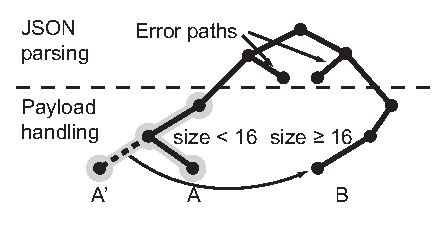
\includegraphics[width=2.4in]{paas/figures/layered-tree}
  \caption{Exploring an execution tree using layered symbolic
    execution.}
  \label{fig:layered-tree}
\end{figure}

Figure~\ref{fig:layered-tree} illustrates an execution tree explored in an iteration of LSE. Consider an initial input for the example in Figure~\ref{fig:test-lpt}, where the value of the $\codebit{size}$ field in the JSON request payload is $8$ (Path $A$ in the figure).
%
At step 2 of the algorithm, a symbolic value is injected for $\codebit{size}$, together with the rest of the onion object wildcard fields (the highlighted segment of Path $A$).  Now, if the tested path contains the conditional statement \codebit{if payload.size < 16}, the \codebit{then} branch of the statement is taken and the $\mathit{size} < 16$ constraint is recorded.  At the end of the execution (step 3), if this constraint is negated to $\mathit{size} \geq 16$, a new value for $\codebit{size}$ is generated, say $20$ (the alternate potential Path $A'$).  Then, at step 4, the \codebit{reconstruct} functions assembles the new values of all leaves into a new HTTP packet to be sent to the app, which will cause the \codebit{else} branch of the \codebit{if} statement to be taken in the next execution (Path $B$).  Note that Path $A'$ is not globally feasible and never explored, but only transiently used to produce the feasible Path $B$.

Compared to a solution that only marks the variables at the layers of interest as symbolic, LSE is superior in two ways: (1)~By obtaining the root input, it is able to run integration tests for a fully deployed application; (2)~LSE supports data structures of variable sizes, e.g., arrays whose lengths are symbolic values, by regenerating the input structure at each new iteration.


%%% Local Variables: 
%%% mode: latex
%%% eval: (visual-line-mode)
%%% fill-column: 1000000
%%% TeX-master: "main"
%%% End:


\section{A Testing Platform for the Cloud}
\label{sec:paas:fedsymbex}
We deploy LSE inside a symbolic execution-aware virtual machine (the symbolic VM) that encapsulates the ``entire universe'' of the application, including the framework and even the language interpreter and operating system, enabling integration testing of the entire application stack.
%
The test-mode deployment then requires just the push of a button for the system to execute the layered parameterized tests, generate coverage statistics, and highlight any failing test cases.

This deployment model leverages the properties of PaaS in several ways:
%
(1)~By hiding the testing VMs behind a service interface, the PaaS system can faithfully reproduce the exact environment of production VMs inside the testing VMs without exposing its internals.
%
(2)~The testing task can be transparently scaled across multiple VMs by using parallel symbolic execution~\cite{cloud9}.
%
(3)~Since the application uses standard interfaces for accessing the PaaS components (storage, networking, etc.), the provider is able to substitute production-optimized implementations with testing-optimized stubs that offer a simplified behavior that is better suited to automated program analysis.

From the perspective of the PaaS provider, the test runner service consists of a set of symbolic VMs, operated separately from the production infrastructure.  When an application is deployed in test mode, one of the symbolic VMs is allocated for testing: the application code and tests are copied to the guest, and the LSE algorithm is invoked.

\paragraph{Architecture}

\begin{figure}
  \centering
  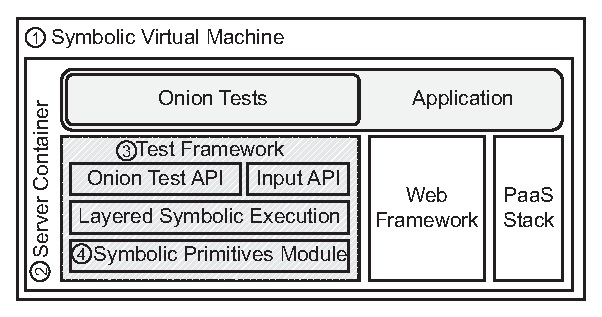
\includegraphics[width=0.7\textwidth]{paas/figures/symbolic-vm}
  \caption{The PaaS test runner service.}
  \label{fig:fse}
\end{figure}

Figure~\ref{fig:fse} illustrates the architecture of the symbolic VM environment.  Inside the VM~\cI, all application components are symbolically executed in the same low-level representation (e.g., x86 machine code or LLVM~\cite{llvm}).  The components execute inside their own vanilla interpreters~\cII.
%
The test framework~\cIII plays two roles: it implements (1) the APIs for LPTs and onion objects that developers use to write the testing code, and (2) the LSE algorithm that guides the test case generation.

\paragraph{Prototype}

We implemented a prototype of the symbolic VM that tests Python-based Google App Engine PaaS applications and is built on top of the S2E symbolic virtual machine.

In our implementation, the symbolic execution engine and the LSE logic live at different levels in the symbolic VM stack.
%
The symbolic execution engine operates with low-level abstractions such as memory bytes. It resides on the host level, as an S2E plugin that exposes the core symbolic execution primitives to the guest as S2E system calls, e.g., to allow marking memory buffers as symbolic.
%
The LSE algorithm operates on web application state (e.g., by accessing the onion objects), and is implemented in the guest as a native Python extension module.  We implemented LSE on top of WebTest~\cite{py-webtest}, a popular fixture library for testing Python web applications.
%
The resulting system is extensible to other languages with limited engineering effort: since the symbolic execution logic is provided at the host level, only the test framework component needs to be implemented in the cloud app language.

Early experiences with the prototype are encouraging: for the full application stack of a simple cloud app, our prototype generates a test case every few seconds.

%%% Local Variables: 
%%% mode: latex
%%% eval: (visual-line-mode)
%%% fill-column: 1000000
%%% TeX-master: "main"
%%% End:





%%% Local Variables: 
%%% mode: latex
%%% eval: (visual-line-mode)
%%% fill-column: 1000000
%%% TeX-master: "main"
%%% End:


\chapter{Evaluation}
\label{ch:evaluation}
The goal of \chef and \cnine is to perform efficient and effective symbolic execution on real-world software targets with complex environment interfaces.
%
In this chapter, after presenting the prototypes for \cnine (Section~\ref{sec:eval:cnine-proto}) and \chef (Section~\ref{sec:eval:chef-proto}), we present our methodology (Section~\ref{sec:eval:methodology}) and answer the following questions:
\begin{enumerate}
\item Can \chef and \cnine symbolically execute real-world software (Section~\ref{sec:eval:targets})?
\item Are the symbolic execution engines effective for bug finding and test suite generation (Section~\ref{sec:eval:bug-finding})?
\item Given the overhead of using the language interpreter, how efficient is \chef's test suite generation (Section~\ref{sec:eval:chef-efficiency})?
\end{enumerate}

\section{The \cnine Prototype}
\label{sec:eval:cnine-proto}

We developed a \cnine prototype on top of the \klee~\cite{klee} symbolic execution engine.  The prototype has 7 \kloc.
%
The \klee modifications to support the symbolic OS abstractions amount to roughly 2 \kloc, while the rest consists of the POSIX model built on top of the abstractions.
%
In addition, we implemented support for parallelizing symbolic execution on a cluster of nodes (Section~\ref{sec:paas:parsymbex}).

\begin{figure}[h!]
  \centering
  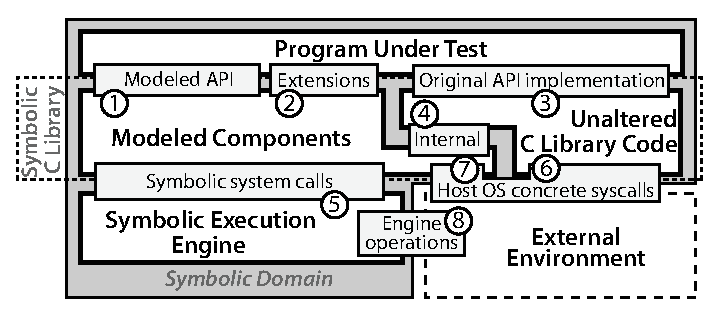
\epsfig{file=evaluation/figures/posix-model.eps, width=6in}
  \caption{Architecture of the \cnine POSIX model.}
  \label{fig:cloud9:posixmodel}
\end{figure}

\cnine builds upon the \klee symbolic execution engine, and so it inherits from \klee the mechanism for replacing parts of the C Library with model code; it also inherits the external calls mechanism.  \cnine adds the symbolic system call interface and replaces parts of the C Library with the POSIX model.  The resulting architecture is shown in Figure~\ref{fig:cloud9:posixmodel}.

\newcommand{\cI}{\!{\raisebox{-0.2ex}{\large\ding{192}}}\xspace}
\newcommand{\cII}{\!{\raisebox{-0.2ex}{\large\ding{193}}}\xspace}
\newcommand{\cIII}{\!{\raisebox{-0.2ex}{\large\ding{194}}}\xspace}
\newcommand{\cIV}{\!{\raisebox{-0.2ex}{\large\ding{195}}}\xspace}
\newcommand{\cV}{\!{\raisebox{-0.2ex}{\large\ding{196}}}\xspace}
\newcommand{\cVI}{\!{\raisebox{-0.2ex}{\large\ding{197}}}\xspace}
\newcommand{\cVII}{\!{\raisebox{-0.2ex}{\large\ding{198}}}\xspace}
\newcommand{\cVIII}{\!{\raisebox{-0.2ex}{\large\ding{199}}}\xspace}

Before symbolic execution starts, the \cnine system links the program under test with a special symbolic C Library.
%
We built this library by replacing parts of the existing uClibc library in \klee with the POSIX model code.  Developers do not need to modify the code of to-be-tested programs in any way to make it run on \cnine.  

In the C Library, we replaced operations related to threads, processes, file descriptors, and network operations with their corresponding model \cI, and augmented the API with \cnine-specific extensions \cII.
%
A large portion of the C Library is reused, since it works out of the box \cIII (e.g. memory and string operations).  Finally, parts of the original C Library itself use  the modeled code \cIV (e.g., Standard I/O \codebit{stdio} relies on the modeled POSIX file descriptors).

The modeled POSIX components interface with the SEE through symbolic system calls \cV, listed in Table~\ref{table:cloud9:primitives} from Section~\ref{sec:cloud9:primitives}.
%
Occasionally, the unmodified part of the C Library invokes external system calls \cVI, and the model code itself needs support from the host OS \cVII---in order to make sure the external calls do not interfere with the symbolic engine's own operations~\cVIII, such access is limited to read-only and/or stateless operations.  This avoids problems like, for instance, allowing an external \codebit{close()} system call to close a network connection or log file that is actually used by the SEE itself.

\klee uses copy-on-write (CoW) to enable memory sharing between symbolic states.
%
We extend this functionality to provide support for multiple address spaces.
%
We organize the address spaces in an execution state as \emph{CoW domains} that permit memory sharing between processes.
%
A memory object marked as shared by calling \codebit{\cninesuffix\_\allowbreak{}make\_\allowbreak{}shared} is automatically mapped in the address spaces of the other processes within the CoW domain.  Whenever a shared object is modified in one address space, the new version is automatically propagated to the other members of the CoW domain.

%%%%%%%%%%%%%%%%%%%%%%%%%%%%%%%%%%%%%%%%%%%%%%%%%%%%%%%%%%%%%%%%%%%%%%%%%%%%%%%%

\section{The Chef Prototype and Case Studies}
\label{sec:eval:chef-proto}

\begin{figure}
  \centering
  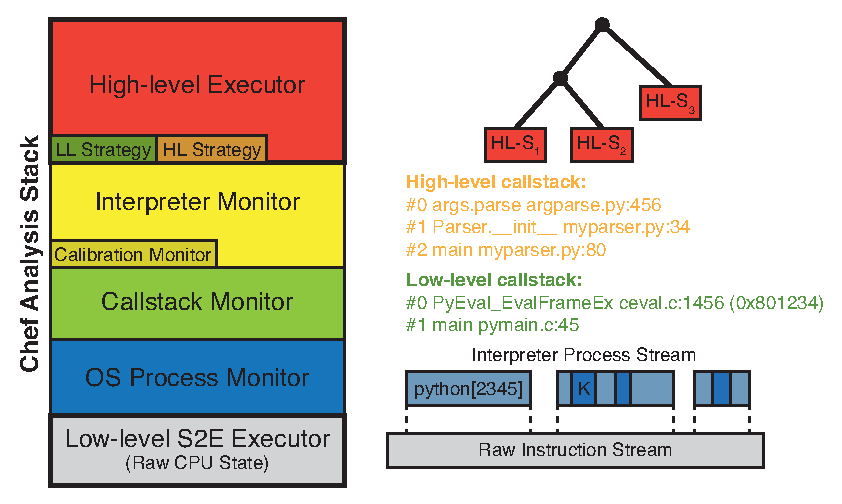
\includegraphics[width=0.7\textwidth]{evaluation/figures/chef-implem-stack}
  \caption{The implementation of \chef, as a stack of S2E analysis modules that refine the raw stream of x86 instructions into a high-level symbolic execution view.}
  \label{fig:eval:chef-implem-stack}
\end{figure}

\paragraph{Implementation}

We implemented \chef on top of the S2E analysis platform~\cite{s2eSystem}, which symbolically executes entire virtual machines.
%
The implementation consists of a stack of dynamic analysis modules that refine the raw stream of x86 instructions at the CPU level into high-level program statements forming a symbolic execution tree (Figure~\ref{fig:eval:chef-implem-stack}).

First, the OS Monitor module breaks down the raw stream of x86 instructions into processes, and separates the user from the kernel mode.
%
The module cooperates with an instrumented Linux kernel in the VM, which reports all running threads, their creation, and termination.  To detect context switches, the OS Monitor tracks the value of the x86 CR3 page table register.  To detect user/kernel mode switches, the OS Monitor tracks the privilege level (ring) in the CPU.
%
The analysis modules above the OS Monitor look only at the user-mode instructions of the interpreter process.

Next, the Callstack Monitor tracks the \codebit{call} and \codebit{ret} instructions in the interpreter to maintain the low-level call stack.
%
On top, the Interpreter Monitor uses the low-level call stack and the interpreter HLPC slice information (Section~\ref{sec:chef:hlcf}) to maintain the high-level HLPC stack.
%
The Interpreter Monitor also computes the HLPC slice when the interpreter runs in calibration mode.

Finally, the top High-level Executor module aggregates the HLPC information from all low-level execution states to maintains the high-level symbolic execution tree.


\paragraph{Case Studies}

We used \chef to generate symbolic execution engines for Python (Section~\ref{sec:eval:python-proto}) and Lua (Section~\ref{sec:eval:lua-proto}). Table~\ref{tab:pychanges} summarizes the effort to set up the two interpreters for \chef.  The necessary changes to the interpreter amount to 321 lines of code for Python and 277 for Lua.
%
The total developer time was 5 person-days for Python and 3 person-days for Lua, which is orders of magnitude smaller than the effort required for building a complete symbolic execution engine from scratch.  

\begin{table}
\centering
\small
\begin{tabular}{|@{\hspace*{4pt}}l@{\hspace*{4pt}}|@{\hspace*{4pt}}r@{\hspace*{4pt}}|@{\hspace*{4pt}}r@{\hspace*{4pt}}|}
\hline
\textbf{Component} & \textbf{Python} & \textbf{Lua}\\
\hline
Interpreter core size (C LoC) & 427,435 & 14,553 \\
\hline
\hline
%% HLPC instrumentation (C LoC) & 47 (0.01\%) & 44 (0.30\%) \\
Sym. optimizations (C LoC) & 274 (0.06\%) & 233 (1.58\%) \\
Native extensions (C LoC) & 1,320 (0.31\%) & 154 (1.06\%) \\
Test library (Python/Lua LoC) & 103 & 87 \\
\hline
\hline
Developer time (person-days) & 5 & 3 \\
\hline
\end{tabular}
\caption{Summary of the effort required to support Python and Lua in \chef.  The first row is the interpreter size without the standard language library. The next row shows changes in the interpreter core, while the following two constitute the symbolic test library.  The last item indicates total developer effort.}
\label{tab:pychanges}
\end{table}

\subsection{Symbolic Execution Engine for Python}
\label{sec:eval:python-proto}

\paragraph{Interpreter Preparation}

We instrumented the CPython interpreter 2.7.3 for use with \chef, according to the guidelines presented in Section~\ref{sec:chef:recipe}.

Python programs are composed of modules, corresponding to Python source files.  Each source file is compiled into an interpreter-specific bytecode format, i.e., each source statement is translated into one or more lower-level primitive instructions.  The instructions are grouped into blocks, corresponding to a single loop nesting, function, method, class, or global module definition.
%
We automatically detect the HLPC variable pointing to the bytecode blocks, by applying the HLPC slice reconstruction procedure in Section~\ref{sec:chef:hlcf}.  We cross-checked the correctness of the obtained slice by looking it up in the interpreter source code, via the debug symbols in the binary.
%% We define an \hlpc as the concatenation of the unique block address of the top frame on the stack and the current instruction offset inside the block. We instrumented the Python interpreter to pass this program location to \chef; this required adding less than 50 LoC to the main interpreter loop.

We performed several optimizations on the Python interpreter: we neutralized the hash functions of strings and integers, which are the most common objects; we concretized the memory sizes passed to the garbage-collected memory allocator; and we eliminated interning for small integers and strings.    
%
Most optimizations involved only adding preprocessor directives for conditional compilation of blocks of code.
%
We gathered the optimizations under a new \codebit{--with-symbex} flag of the interpreter's \codebit{./configure} script.

\paragraph{Symbolic Tests}

To validate the usefulness of the resulting symbolic execution engine, we use it as a test case generation tool.  To this end, we implemented a symbolic test library as a separate Python package, used both inside the guest virtual machine, and outside, during test replay.
%
Figure~\ref{fig:sample-test} is an example of a symbolic test class for the \codebit{argparse} command-line interface generator. It sets up a total of 12 symbolic characters of input: two 3-character symbolic arguments to configure the command-line parser plus another two to exercise the parsing functionality.

The test class derives from the library's \codebit{SymbolicTest} class, which provides two methods to be overridden: \codebit{setUp}, which is run once before the symbolic test starts, and \codebit{runTest}, which creates the symbolic input and can check properties.  The symbolic inputs are created by calling the \codebit{getString} and \codebit{getInt} methods in the \codebit{SymbolicTest} API.

\begin{figure}
  \centering
  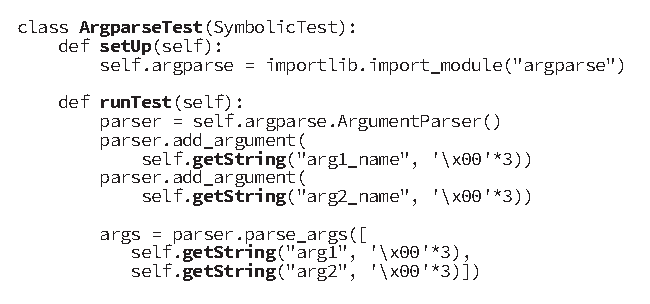
\includegraphics[width=3.2in]{evaluation/figures/symtest}
  \caption{The symbolic test used to exercise the functionality of the Python \codebit{argparse} package.}
  \label{fig:sample-test}
\end{figure}

A symbolic test is executed by a symbolic test runner, which is also part of the library.  The runner can work in either symbolic or replay mode. 
%
In \emph{symbolic mode}, the runner executes inside the guest virtual machine.  It creates a single instance of the test class, whose \codebit{getString} and \codebit{getInt} methods create corresponding Python objects and invoke the \codebit{make\_symbolic} call to mark their memory buffers as symbolic.
%
In \emph{replay mode}, the runner creates one instance of the test class for each test case created by \chef. The \codebit{getString} and \codebit{getInt} methods return the concrete input assignment of the test case.


\subsection{Symbolic Execution Engine for Lua}
\label{sec:eval:lua-proto}

Lua is a lightweight scripting language mainly used as an interpreter library to add scripting capabilities to software written in other languages. However, it also has a standalone interpreter and several Lua-only projects exist. We generated a symbolic execution engine for Lua based on version 5.2.2 of the Lua interpreter.

\paragraph{Interpreter Instrumentation}

Similar to Python, Lua programs are composed of one or more Lua source files, compiled into a bytecode format.  The code is compiled into a set of functions that operate on a global stack of values.  Each function is composed of a sequence of bytecode instructions, where each instruction is defined by an offset, opcode, and parameters.
%
We automatically detect updates to the HLPC variable pointing to bytecode instructions.  We cross-checked the correctness of the interpreter HLPC slice using the debug symbols in the binary.
%% We construct the \hlpc as the concatenation of the unique address of the function in the top frame and the current instruction offset being executed.  The instrumentation amounts to less than 50 LoC added to the interpreter loop.

We optimized the Lua interpreter for symbolic execution by eliminating string interning.  In addition, we configured the interpreter to use integer numbers instead of the default floating point, for which S2E does not support symbolic expressions.  This change was easy, because it was available as a macro definition in the interpreter's configuration header.

%%%%%%%%%%%%%%%%%%%%%%%%%%%%%%%%%%%%%%%%%%%%%%%%%%%%%%%%%%%%%%%%%%%%%%%%%%%%%%%%

\section{Methodology}
\label{sec:eval:methodology}

\paragraph{Hardware Configuration}

For all our \cnine experiments, we ran \cnine in parallel symbolic execution mode in a heterogeneous cluster environment, with worker CPU frequencies between 2.3--2.6 GHz and with 4--6 GB of RAM available per core.

All reported \chef experiments were performed on a 48-core 2.3 GHz AMD Opteron 6176 machine with 512 GB of RAM, running Ubuntu 12.04. Each \chef invocation ran on 1 CPU core and used up to 8 GB of RAM on average.

\paragraph{Coverage Measurement}

Line or statement coverage remains widely used, even though its meaningfulness as a metric for test quality is disputed. We measure and report line coverage to give a sense of what users can expect from a test suite generated fully automatically by \cnine or a symbolic execution engine based on \chef.  For Python, we rely on the popular \codebit{coverage} package, and for Lua we use the \codebit{luacov} package.

Since our \chef prototype only supports strings and integers as symbolic program inputs, we count only the lines of code that can be reached using such inputs. We report this number as ``coverable LOC'' in the fifth column of Table~\ref{tab:targets}, and use it in our experiments as a baseline for what such a symbolic execution engine could theoretically cover directly.  For example, for the \codebit{simplejson} library, this includes only code that decodes JSON-encoded strings, not code that takes a JSON object and encodes it into a string. Note that, in principle, such code could still be tested and covered by writing a more elaborate symbolic test that sets up a JSON object based on symbolic primitives~\cite{paas-testing}.

\paragraph{State Searchers in \cnine}

On each worker, the underlying \klee engine used the best searchers from \cite{klee}, namely an interleaving of random-path and coverage-optimized strategies. At each step, the engine alternately selects one of these heuristics to pick the next state to explore. Random-path traverses the execution tree starting from the root and randomly picks the next descendant node, until a candidate state is reached. The coverage-optimized strategy weighs the states according to an estimated distance to an uncovered line of code, and then randomly selects the next state according to these weights.

%%%%%%%%%%%%%%%%%%%%%%%%%%%%%%%%%%%%%%%%%%%%%%%%%%%%%%%%%%%%%%%%%%%%%%%%%%%%%%%%

\section{Testing Targets}
\label{sec:eval:targets}

\subsection{Testing Low-level Systems with Cloud9}

Table~\ref{table:tested} shows a selection of the systems we tested with \cnine, covering several types of software.  We confirmed that each system can be tested properly under our POSIX model. In the rest of this section, we focus our in-depth evaluation on several networked servers and tools, as they are frequently used in settings where reliability matters.

\begin{table}[h!]
\addtolength{\tabcolsep}{-2pt}
\centering
\small
\begin{tabular}{| l | r@{.}p{1pt} | l |}
\hline
\textbf{~~~~~~~System} & \multicolumn{2}{|l|}{\textbf{Size (\kloc)}} & \textbf{~~~~Type of Software} \\
\hline
Apache httpd 2.2.16 & ~~~~~~~226 & 4 & \multirow{3}{*}{Web servers}\\
Lighttpd 1.4.28         &                 39 & 5 & \\
Ghttpd 1.4.4             &                   0 & 6  & \\ \hline
Memcached 1.4.5     &                   8 & 3 &  Distributed object cache \\\hline
Python 2.6.5             &               388 & 3 & Language interpreter \\ \hline
Curl 7.21.1               &                  65 & 9 & \multirow{2}{*}{Network utilities} \\ 
Rsync 3.0.7               &                  35 & 6 & \\\hline 
Pbzip 2.1.1               &                  3 & 6 & Compression utility \\ \hline
Libevent 1.4.14         &                  10 & 2 & Event notification library \\ \hline
Coreutils 6.10          &                  72 & 1 & Suite of system utilities \\ \hline
Bandicoot 1.0           &                   6 & 4 & Lightweight DBMS \\ \hline
\end{tabular}
\caption{Representative selection of testing targets that run on \cnine.  Size was measured using the \codebit{sloccount} utility.}
\label{table:tested}
\end{table}

Due to its comprehensive POSIX model, \cnine can test many kinds of servers.  One example is lighttpd, a web server used by numerous high-profile web sites, such as YouTube, Wikimedia, Meebo, and SourceForge.  For lighttpd, \cnine proved that a certain bug fix was incorrect, and the bug could still manifest even after applying the patch (Section~\ref{sec:eval:lighttpd}). \cnine also found a bug in curl, an Internet transfer application that is part of most Linux distributions and other operating systems (Section~\ref{sec:eval:curl}).  \cnine also found a hang bug in the UDP handling code of memcached, a distributed memory object cache system used by many Internet services, such as Flickr, Craigslist, Twitter, and Livejournal (Section~\ref{sec:eval:memcached}).

In addition to the testing targets mentioned above, we also tested a benchmark consisting of a multi-threaded and multi-process producer-consumer simulation. The benchmark exercises the entire functionality of the POSIX model: threads, synchronization, processes, and networking. 

We conclude that \cnine is practical and capable of testing a wide range of real-world software systems.


\subsection{Testing Python and Lua Packages with Chef}

\begin{table*}[!ht]
\centering
\footnotesize
\begin{tabular}{@{\hspace*{5pt}}l@{\hspace*{11pt}}r@{\hspace*{11pt}}l@{\hspace*{11pt}}l|r|c|c@{\hspace*{5pt}}}
\textbf{Package} & \textbf{LOC} & \textbf{Type} & \textbf{Description} & \textbf{Coverable LOC} & \textbf{Exceptions} & \textbf{Hangs}\\
\hline
\rule{0pt}{12pt}\textbf{Python} & & & & & \\
argparse$^{*}$ & 1,466 & System & Command-line interface & 1,174 & 4 / 0 & --- \\
ConfigParser$^{*}$ & 451 & System & Configuration file parser & 145 & 1 / 0 & --- \\
%
HTMLParser$^{*}$ & 623 & Web & HTML parser & 582 & 1 / 0 & --- \\
simplejson 3.10 & 1,087 & Web & JSON format parser & 315 & 2 / 0 & --- \\
%% webapp2 2.5.2 & 1,986 & Web & Web framework & & \\
%
unicodecsv 0.9.4 & 126 & Office & CSV file parser & 95 & 1 / 0 & --- \\
xlrd 0.9.2 & 7,241 & Office & Microsoft Excel reader & 4,914 & 5 / 4 & --- \\[2pt]
%
\hline
\rule{0pt}{12pt}\textbf{Lua} & & & & & & \\
cliargs 2.1-2 & 370 & System & Command-line interface & 273 & --- & --- \\
haml 0.2.0-1 & 984 & Web & HTML description markup & 775 & --- & --- \\
sb-JSON v2007 & 454 & Web & JSON format parser & 329 & --- & $\checkmark$ \\
markdown 0.32 & 1,057 & Web & Text-to-HTML conversion & 673 & --- & --- \\
moonscript 0.2.4-1 & 4,634 & System & Language that compiles to Lua & 3,577 & --- & --- \\[2pt]
%
\hline
\rule{0pt}{12pt}\textbf{TOTAL} & 18,493 & & & 12,852 & & \\
\end{tabular}
\caption{Summary of testing results for the Python and Lua packages
  used for evaluation. Items with (*) represent standard library
  packages.
  Exception numbers indicate total / undocumented exception types
  discovered.}
\label{tab:targets}
\end{table*}

We evaluated the symbolic execution engines for Python and Lua on 6 Python and 5 Lua packages, respectively, including system, web, and office libraries. In total, the tested code in these packages amounts to about $12.8$ KLOC.  We chose the latest versions of widely used packages from the Python standard library, the Python Package Index, and the Luarocks repository.  Whenever possible, we chose the pure interpreted implementation of the package over the native optimized one (e.g., the Python \codebit{simplejson} package). The first five columns of Table~\ref{tab:targets} summarize the package characteristics; LOC numbers were obtained with the \codebit{cloc} tool~\cite{cloc}.

The reported package sizes exclude libraries, native extension modules, and the packages' own test suites.
However, the packages ran in their unmodified form, using all the language features and libraries they were designed to use, including classes, built-in data structures (strings, lists, dictionaries), regular expressions, native extension modules, and reflection.  

All testing targets have a significant amount of their functionality written in the interpreted language itself; we avoided targets that are just simple wrappers around native extension modules (written in C or C++) in order to focus on the effectiveness of \chef at distilling high-level paths from low-level symbolic execution.  Nevertheless, we also included libraries that depend on native extension modules.  For instance, all the testing targets containing a lexing and parsing component use Python's standard regular expression library, which is implemented in C.
% The execution of parsers heavily depends on possible regular expression matches on input strings.
To thoroughly test these parsers, it is important to also symbolically execute the native regular expression library. For this, the binary symbolic execution capabilities of \chef are essential.

\paragraph{Symbolic Tests}

For each package, we wrote a symbolic test that invokes the package's entry points with one or more symbolic strings.  
%The symbolic tests invoke the code under test in a generic manner without specific checks.  
Figure~\ref{fig:sample-test} in Section~\ref{sec:eval:python-proto} is an example of such a symbolic test.

Each symbolic test ran for 30 minutes within \chef, after which we replayed the collected high-level tests on the host machine, in a vanilla Python/Lua environment, to confirm test results and measure line coverage.  To compensate for the randomness in the state selection strategies, we repeated each experiment 15 times.  In each graph we present average values and error margins as +/- one standard deviation.

For our experiments, we did not use explicit specifications, but relied on generic checks for finding common programming mistakes.  For both Python and Lua, we checked for interpreter crashes and potential hangs (infinite loops). 
For Python---which, unlike Lua, has an exception mechanism---we also flagged whenever a test case led to unspecified exceptions being thrown.
%
In general, one could find application-specific types of bugs by adding specifications in the form of assertions, as in normal unit tests.

%%%%%%%%%%%%%%%%%%%%%%%%%%%%%%%%%%%%%%%%%%%%%%%%%%%%%%%%%%%%%%%%%%%%%%%%%%%%%%%%

\section{Effectiveness for Bug Finding and Test Generation}
\label{sec:eval:bug-finding}

In this section we present several case studies that illustrate how \cnine and \chef can explore and find new bugs. %% confirm/disprove that existing bugs have been correctly fixed, and regression-test a program after it has been modified.  In the common case, \cnine users start with a concrete test case (e.g., from an existing test suite) and generalize it by making data symbolic and by controlling the environment.

%--------------------------------------------------
\subsection{Case Study \#1: Curl}
\label{sec:eval:curl}

Curl is a popular data transfer tool for multiple network protocols, including HTTP and FTP.  When testing it, \cnine\ found a new bug which causes Curl to crash when given a URL regular expression of the form ``\codebit{http://site.\{one,two,three\}.com\{}''. \cnine exposed a general problem in Curl's handling of the case when braces used for regular expression globbing are not matched properly.  The bug was confirmed and fixed within 24 hours by the developers. 

This problem had not been noticed before because the globbing functionality in Curl was shadowed by the same functionality in command-line interpreters (e.g., Bash).  This case study illustrates a situation that occurs often in practice: when a piece of software is used in a way that has not been tried before, it is likely to fail due to latent bugs.

\subsection{Case Study \#2: Memcached}
\label{sec:eval:memcached}

Memcached is a distributed memory object cache system, mainly used to speed up web application access to persistent
data, typically residing in a database. % Memcached is deployed at many large sites like Facebook, Twitter, and YouTube. 

Memcached comes with an extensive test suite comprised of C and Perl code. Running it completely takes about 1 minute; it runs 6,472 different test cases  and explores $83.66\%$ of the code. While this is considered thorough by today's standards, two easy \cnine\ test cases further increased code coverage. Table~\ref{table:memcached} contains a summary of our results, presented in more details in the following paragraphs.


\paragraph{Symbolic Packets}

The memcached server accepts commands over the network. Based on memcached's C test suite, we wrote a test case that sends memcached a generic, symbolic binary command (i.e., command content is fully symbolic), followed by a second symbolic command. This test captures all operations that entail a pair of commands.

A 24-worker \cnine\ explored in less than 1 hour all 74,503 paths associated with this sequence of two symbolic packets, covering an additional 1.13\% of the  code relative to the original test suite.  What we found most encouraging in this result is that such exhaustive tests constitute first steps toward using symbolic tests to \emph{prove} properties of real-world programs, not just to look for bugs.  Symbolic tests may provide an alternative to complex proof mechanisms that is more intuitive for developers and thus more practical.

\paragraph{Symbolic Fault Injection}

We also tested memcached with fault injection enabled, whereby we injected all feasible failures in memcached's calls to the C Standard Library.  After 10 minutes of testing, a 24-worker \cnine\ explored 312,465 paths, adding $1.28\%$ over the base test suite.  The fact that {\em line} coverage increased by so little, despite having covered almost $50\times$ more paths, illustrates the weakness of line coverage as a metric for test quality---high line coverage should offer no high confidence in the tested code's quality.

For the fault injection experiment, we used a special strategy that sorts the execution states according to the number of faults recorded along their paths, and favors the states with fewer fault injection points. This led to a uniform injection of faults: we first injected one fault in every possible fault injection point along the original C test suite path, then injected pairs of faults, and so on.  We believe this is a practical approach to using fault injection as part of regular testing.

\begin{table}
\small
\centering
\addtolength{\tabcolsep}{-1.3pt}
\begin{tabular}{| p{2.3cm} | r | c | c | }
\hline
{\bf Testing Method}   & {\bf Paths}~~       & {\bf Isolated}             & {\bf Cumulated}          \\ 
                                & {\bf  Covered}  & {\bf Coverage$^{*}$} & {\bf Coverage$^{**}$}      \\
\hline
Entire test suite               & 6,472         & $83.67\%$        &---                   \\
\hline
\raggedright Binary protocol test suite      & 27            & $46.79\%$        & $84.33\%$ ($+0.67\%$) \\
\hline
Symbolic packets                & 74,503        & $35.99\%$        & $84.79\%$ ($+1.13\%$) \\
\hline
\raggedright Test suite + fault~injection    & 312,465       & $47.82\%$        & $84.94\%$ ($+1.28\%$) \\
\hline
\end{tabular}
\caption{Path and code coverage increase obtained by each symbolic testing technique on memcached. We show total coverage obtained with each testing method (*), as well as total coverage obtained by augmenting the original test suite with the indicated method  (**); in parentheses, we show the increase over the entire test suite's coverage.}
\label{table:memcached}
% \vspace{-0.3cm}
\end{table}

\paragraph{Hang Detection}

We tested memcached with symbolic UDP packets, and \cnine discovered a hang condition in the packet parsing code: 
when a sequence of packet fragments of a certain size arrive at the server, memcached enters an infinite loop, which prevents it from serving any further UDP connections. This bug can seriously hurt the availability of infrastructures using memcached.

We discovered the bug by limiting the maximum number of instructions executed per path to $5 \times 10^6$.  The paths without the bug terminated after executing $\approximately 3\times 10^5$ instructions; the other paths that hit the maximum pointed us to the bug.

%--------------------------------------------------
\subsection{Case Study \#3: Lighttpd}
\label{sec:eval:lighttpd}


The lighttpd web server is specifically engineered for high request throughput, and it is quite sensitive to the rate at which new data is read from a socket.  Alas, the POSIX specification offers no guarantee on the number of bytes that can be read from a file descriptor at a time.  lighttpd 1.4.12 has a bug in the command-processing code that causes the server to crash (and connected clients to hang indefinitely) depending on how the incoming stream of requests is fragmented. 

We wrote a symbolic test case to exercise different \emph{stream fragmentation} patterns and see how different lighttpd versions behave. We constructed a simple HTTP request, which was then sent over the network to lighttpd. We activated network packet fragmentation via the symbolic \codebit{ioctl()}  API explained in Section~\ref{sec:cloud9:symtests}. We confirmed that certain fragmentation patterns cause lighttpd to crash (prior to the bug fix). However, we also tested the server right after the fix and discovered that the bug fix was incomplete, as some fragmentation patterns still cause a crash and hang the client (Table~\ref{table:lighttpd}).

This case study shows that \cnine can find bugs caused by specific interactions with the environment which are hard to test with a concrete test suite. It also shows how \cnine can be used to write effective regression test suites---had a stream-fragmentation symbolic test been run after the fix, the lighttpd developers would have promptly discovered the incompleteness of their fix.

\begin{table}
\small
\centering
\begin{tabular}{| p{3.8cm} | p{1.65cm} | p{1.65cm} |}
\hline
\bf Fragmentation pattern & \bf ver. 1.4.12 & \bf ver. 1.4.13 \\
\bf (data sizes in bytes) & \bf (pre-patch)     & \bf (post-patch)\\
\hline
$1 \times 28$ 			& 		OK		& OK \\
\hline
$1 \times 26 + 1 \times 2$  & crash + hang 	& OK \\
\hline
$2+5+1+5+2 \times 1 + 3 \times 2 + 5 + 2 \times 1 $	& crash + hang 	& crash + hang \\
\hline
\end{tabular}
\caption{The behavior of different versions of lighttpd to three ways of fragmenting the HTTP request "GET /index.html HTTP/1.0\textsc{Cr}\textsc{Lf}\textsc{Cr}\textsc{Lf}" (string length 28).}
\label{table:lighttpd}
\end{table}

\subsection{Case Study \#4: Bandicoot DBMS}
\label{sec:eval:bandicoot}

Bandicoot is a lightweight DBMS that can be accessed over an HTTP interface.  We exhaustively explored all paths handling the GET commands and found a bug in which Bandicoot reads from outside its allocated memory.  The particular test we ran fortuitously did not result in a crash, as Bandicoot ended up reading from the libc memory allocator's metadata preceding the allocated block of memory. However, besides the read data being wrong, this bug could cause a crash depending on where the memory block was allocated.

To discover and diagnose this bug without \cnine is difficult. First, a concrete test case has little chance of triggering the bug.  Second, searching for the bug with a sequential symbolic execution tool seems impractical: the exhaustive exploration took 9 hours with a 4-worker \cnine (and less than 1 hour with a 24-worker cluster). 

\subsection{Comparing \cnine to KLEE}

\cnine inherits \klee's capabilities, being able to recognize memory errors and failed assertions. We did not add much in terms of bug detection, only two mechanisms for detecting hangs: check if all symbolic threads are sleeping (deadlock) and set a threshold for the maximum number of instructions executed per path (infinite loop or livelock).  Even so, \cnine can find bugs beyond \klee's abilities because the POSIX model allows \cnine to reach more paths and explore deeper portions of the tested program's code---this exposes additional potentially buggy situations. \cnine also has more total memory and CPU available, due to its distributed nature, so it can afford to explore more paths than \klee.  As we have shown above, it is feasible to offer proofs for certain program properties: despite the exponential nature of exhaustively exploring paths, one can build small but useful symbolic test cases that can be exhaustively executed.


\subsection{Case Study \#5: Exploratory Bug Finding in Python and Lua Packages}
\label{sec:eval:bug-explore}

We now evaluate the effectiveness of the \chef-obtained symbolic execution engines for bug detection.

The specifications we used for our experiments are application-agnostic and only check for per-path termination within a given time bound and for the absence of unrecoverable crashes.  The first specification checks whether a call into the runtime returns within 60 seconds.  In this way, we discovered a bug in the Lua JSON package that causes the parser to hang in an infinite loop: if the JSON string contains the \codebit{/*} or \codebit{//} strings marking the start of a comment but no matching \codebit{*/} or line terminator, the parser reaches the end of the string and continues spinning waiting for another token.
%
This bug is interesting for two reasons: First, comments are not part of the JSON standard, and the parser accepts them only for convenience, so this is a clear case of an interpreter-specific bug.  Second, JSON encodings are normally automatically generated and transmitted over the network, so they are unlikely to contain comments; traditional testing is thus likely to miss this problem. However, an attacker could launch a denial of service attack by sending a JSON object with a malformed comment.

The second implicit specification checks that a program never terminates non-gracefully, i.e., the interpreter implementation or a native extension crashes without giving the program a chance to recover through the language exception mechanisms.  In our experiments, our test cases did not expose any such behavior.


\subsection{Case Study \#6: Undocumented Exceptions in Python Packages}
\label{sec:eval:undoc-except}

This scenario focuses on finding undocumented exceptions in Python code.
%
Being memory-safe languages, crashes in Python and Lua code tend to be due to \emph{unhandled exceptions} rather than bad explicit pointers.  When such exceptions are not caught by the program, they propagate to the top of the stack and cause the program to be terminated prematurely. 
%
In dynamic languages, it is difficult to determine all the possible exceptions that a function can throw to the callee, because there is no language-enforced type-based API contract.  Users of an API can only rely on the documentation or an inspection of the implementation.  Therefore, undocumented exceptions are unlikely to be checked for in \codebit{try}-\codebit{except} constructs and can erroneously propagate further.
%
They can then hurt productivity (e.g., a script that crashes just as it was about to complete a multi-TB backup job) or disrupt service (e.g., result in an HTTP 500 Internal Server Error).

We looked at all the Python exceptions triggered by the test cases generated using \chef and classified them into \emph{documented} and \emph{undocumented}.  The documented exceptions are either exceptions explicitly mentioned in the package documentation or common Python exceptions that are part of the standard library (e.g., \codebit{KeyError}, \codebit{ValueError}, \codebit{TypeError}).  Undocumented exceptions are all the rest.

The sixth column in Table~\ref{tab:targets} summarizes our findings.  We found four undocumented exceptions in \codebit{xlrd}, the largest package.  These exceptions occur when parsing a Microsoft Excel file, and they are \codebit{BadZipfile}, \codebit{IndexError}, \codebit{error}, and \codebit{AssertionError}.  These errors occur inside the inner components of the Excel parser, and should have either been documented or, preferably, been caught by the parser and re-raised as the user-facing \codebit{XLRDError}.

%%%%%%%%%%%%%%%%%%%%%%%%%%%%%%%%%%%%%%%%%%%%%%%%%%%%%%%%%%%%%%%%%%%%%%%%%%%%%%%%

\section{Efficiency of Test Generation with \chef}
\label{sec:eval:chef-efficiency}

\subsection{Impact of \cupa Heuristics and Interpreter Optimizations}
\label{sec:sub:perf-cupa}

We now analyze the impact of the \cupa heuristics (described in Section~\ref{sec:chef:cupa}) and the interpreter optimizations (described in Section~\ref{sec:chef:optimizeforsymbex}) on test generation effectiveness.  Specifically, we measure the number of paths (respectively source code lines) covered by the test suite generated in 30 minutes for the packages in Table~\ref{tab:targets}.

We compare the results obtained in 4 different configurations: (1) the baseline, consisting of performing random state selection while executing the unmodified interpreter, and then either use (2) the path- or coverage-optimized CUPA only, (3) the optimized interpreter only, or (4) both CUPA and the optimized interpreter.  This way we measure the individual contribution of each technique, as well as their aggregate behavior.

\paragraph{Test Case Generation}

Figure~\ref{fig:tc-improv} compares the number of test cases generated with each of the 4 \chef configurations, using the path-optimized CUPA~(Section~\ref{sec:chef:cupa-paths}).  We only count the \textit{relevant} high-level test cases, that is, each test case exercises a unique high-level path in the target Python program.

\begin{figure}[t]
  \centering
  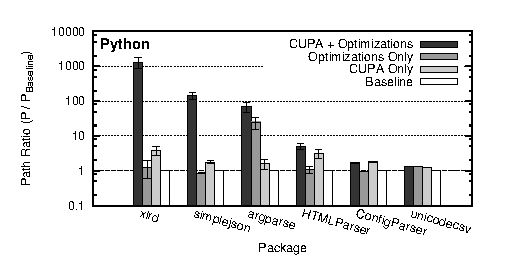
\includegraphics[width=3.27in]{evaluation/graphs/chef/bkdown-path-python} \\
  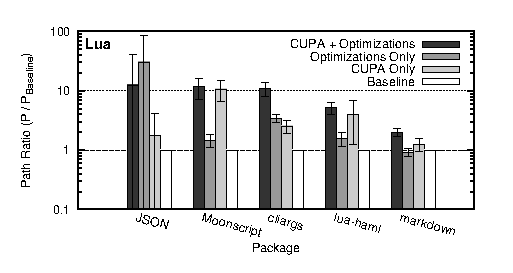
\includegraphics[width=3.27in]{evaluation/graphs/chef/bkdown-path-lua}
  \caption{The number of Python and Lua test cases generated by
    coverage- and path-optimized \cupa relative to random state
    selection (logarithmic scale).}
  \label{fig:tc-improv}
\end{figure}

For all but one of the 11 packages (6 Python plus 5 Lua), the aggregate CUPA + interpreter optimizations performs the best, often by a significant margin over the baseline.  This validates the design premises behind our techniques.

The CUPA strategy and the interpreter optimizations may interact non-linearly.  In two cases (Python's \codebit{xlrd} and \codebit{simplejson}), the aggregate significantly outperforms either individual technique. These are cases where the result is better than the sum of its parts.  In the other cases, the result is roughly the sum of each part, although the contribution of each part differs among targets.  This is visually depicted on the log-scale graph: for each cluster, the heights of the middle bars measured from level $1 \times$ roughly add up to the height of the aggregate (left) bar.

In one case (Lua's \codebit{JSON}), the aggregate performs worse on average than using the interpreter optimizations alone.  Moreover, the performance of each configuration is less predictable, as shown by the large error bars.  This behavior is due to the generated tests that cause the interpreter to hang, as explained in Section~\ref{sec:eval:bug-finding}.  To detect hangs, the test runs for 60 seconds before switching to another test case.  This acts as a ``penalty'' for the configurations that find more paths leading to the hang and also skews the distribution of path execution times, since the hanging paths take significantly longer than the normal (terminating) paths.

\paragraph{Line Coverage}

Figure~\ref{fig:coverage-improv} shows the line coverage achieved by each configuration, using CUPA optimized for line coverage (Section~\ref{sec:chef:cupa-coverage}).  In 6 out of 11 packages, the coverage improvement is noticeable, and for Python's \codebit{simplejson} and \codebit{xlrd}, the improvements are significant ($80\%$ and $40\%$).

Note that these coverage improvements are obtained using basic symbolic tests that do not make assumptions about the input format.  We believe that tailoring the symbolic tests to the specifics of each package could improve these results significantly.

\begin{figure}[t]
  \centering
  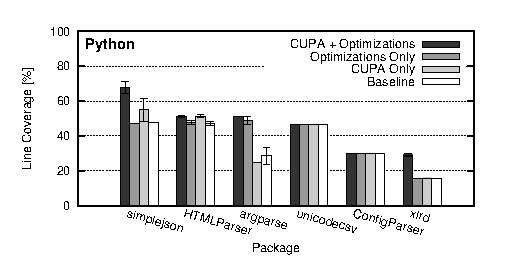
\includegraphics[width=3.2in]{evaluation/graphs/chef/bkdown-stmtcov-python} \\
  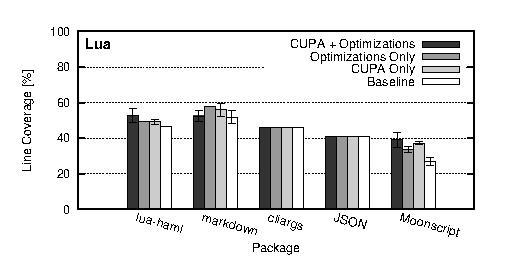
\includegraphics[width=3.2in]{evaluation/graphs/chef/bkdown-stmtcov-lua}
  \caption{Line coverage for the experiments of Figure~\ref{fig:tc-improv}.}
  \label{fig:coverage-improv}
\end{figure}

\subsection{Breaking Down Chef's Interpreter Optimizations}
\label{sec:sub:optimizations}

We now analyze in more depth the impact of the interpreter optimizations by breaking them down into the three types mentioned in Section~\ref{sec:chef:optimizeforsymbex}: avoiding symbolic pointers, hash neutralization, and fast-path elimination.  We run again the symbolic tests for 30 minutes, using the path-optimized CUPA and four different interpreter builds, starting from the vanilla interpreter and adding the optimization types one by one.  For each build and package, we count the number of high-level paths discovered by \chef.

Figure~\ref{fig:optimizations} shows the results for Python.  The data is normalized such that the number of high-level paths for each target reaches $100\%$.  For 3 out of 6 packages (\codebit{simplejson}, \codebit{argparse}, and \codebit{HTMLParser}), \chef's performance monotonically increases as more optimizations are introduced.  For \codebit{unicodecsv} and \codebit{ConfigParser}, the optimizations do not bring any benefits or even hurt slightly.  

However, in the case of \codebit{xlrd}, hash neutralization and fast path elimination seem to actually \emph{hurt} symbolic execution, since the best performance is attained when only symbolic pointer avoidance is in effect.  We explain this behavior by the fact that the different optimization levels cause the search strategy to explore different behaviors of the target package.  \codebit{xlrd} is by far the largest Python package in our evaluation (7.2KLOC vs. the second largest of 1.4KLOC) and includes a diverse set of behaviors, each with its own performance properties.

This result suggests that, for large packages, a \emph{portfolio} of interpreter builds with different optimizations enabled would help further increase the path coverage.

\begin{figure}
  \centering
  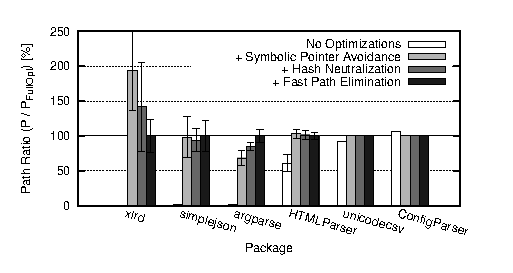
\includegraphics[width=3.2in]{evaluation/graphs/chef/optimizations-bars-python}
  \caption{The contribution of interpreter optimizations for Python as number of high-level paths explored.  Number of paths is relative to full optimizations ($100\%$) for each package.}
  \label{fig:optimizations}
\end{figure}


\subsection{Comparing Chef Against Hand-Made Engines}
\label{sec:sub:comparison}

We now evaluate the trade-offs in using a symbolic execution engine generated with \chef over building one ``by hand''.

\paragraph{Hand-Made Engines}

To our knowledge, no symbolic execution engine for Lua exists.  For Python, we found three research tools, which we compare \chef to.  (1) \cutiepy~\cite{cutie-py} is a concolic engine based on a formal model of the Python language.  It uses a custom CPython interpreter to drive a concrete execution, along with updating the symbolic state according to model semantics. (2) NICE-PySE~\cite{nice} is part of the NICE framework for testing OpenFlow applications.  We will refer to it as \nicese, for brevity. It wraps supported data types into symbolic counterparts that carry the symbolic store, and uses Python's tracing mechanisms to implement the interpretation loop fully in Python.  (3) The symbolic execution engine of the scalability testing tool Commuter~\cite{commuter} is also entirely built in Python.  Its primary purpose is the construction of models that explicitly use an API of symbolic data types.

We perform our comparison along three aspects: language features supported, implementation faithfulness, and performance.  The last two aspects are evaluated only against \nicese, which, besides being open source, is most compatible with our symbolic data representation (based on STP~\cite{stp}).

\paragraph{Language Feature Support}

Table~\ref{tab:langfeats} summarizes the language feature support for \chef, \nicese, \cutiepy, and \commuterse, as implemented at the moment of writing.  We relied on information from the respective papers in all cases and additionally on the implementation in the cases of \nicese and \commuterse, which are available as open source.

We distinguish engines designed to support arbitrary Python code (the ``Vanilla'' label) and those where the symbolic data types are an API used by model code (the ``Model'' label).  Engines in the ``Model'' category essentially offer a ``symbolic domain-specific language'' on top of the interpreted language.  \chef, \cutiepy, and \nicese are ``vanilla'' engines, since their testing targets do not have to be aware that they are being symbolically executed.  \commuterse is a model-based engine, since its testing targets are bound to the symbolic API offered by the engine.

We grouped the supported language features into program state representation (the language data model and types) and manipulation (the operations on data).  We divide data types into values (integers, strings and floating-point), collections (lists and dictionaries), and user-defined classes.  The operations consist of data manipulation, basic control flow (e.g., branches, method calls), advanced control flow (e.g., exception handling, generators), and native method invocations (they are atomic operations at the high level).  We also include in the comparison the ability to execute unsupported operations in concrete-only mode.


% Some names unlikely to clash with other definitions...
\newcommand{\compsupp}{\ensuremath{\CIRCLE}}
\newcommand{\partsupp}{\ensuremath{\LEFTcircle}}
\newcommand{\unsupp}{\ensuremath{\Circle}}

\begin{table}[tb]
\centering
\small
\begin{tabular}{@{\hspace*{2pt}}l@{\hspace*{2pt}} | @{\hspace*{2pt}}c@{\hspace*{2pt}} | @{\hspace*{2pt}}c@{\hspace*{2pt}} | @{\hspace*{2pt}}c@{\hspace*{2pt}} | @{\hspace*{2pt}}c@{\hspace*{2pt}}}
                    & \textbf{\chef}            & \textbf{\cutiepy} & \textbf{\nicese} & \textbf{\commuterse} \\
\hline
\rule{0pt}{12pt}\textbf{Engine type}& Vanilla   & Vanilla    & Vanilla   & Model       \\
\rule{0pt}{12pt}\textbf{Data types} &           &            &           &             \\
Integers            & $\compsupp^{\hphantom{*}}$  & \compsupp  & \compsupp  & \compsupp  \\
Strings             & $\compsupp^{\hphantom{*}}$  & \unsupp    & \unsupp    & \partsupp  \\
Floating point      & $\unsupp^{\hphantom{*}}$    & \unsupp    & \unsupp    & \unsupp    \\
Lists and maps      & $\compsupp^{*}$           & \partsupp   & \unsupp    & \compsupp  \\
User-defined classes& $\compsupp^{*}$           & \unsupp     & \partsupp   & \partsupp \\
\rule{0pt}{12pt}\textbf{Operations}   &                          &            &            &             \\
Data manipulation     & $\compsupp^{\hphantom{*}}$ & \partsupp  &  \partsupp & \partsupp   \\
Basic control flow    & $\compsupp^{\hphantom{*}}$ & \compsupp  &  \partsupp & \compsupp   \\
Advanced control flow & $\compsupp^{\hphantom{*}}$ & \compsupp  &  \unsupp   & \compsupp   \\
Native methods        & $\compsupp^{\hphantom{*}}$ & \partsupp  &  \unsupp   & \unsupp     \\
\end{tabular}
\rule{0pt}{12pt}\compsupp Complete \hspace{12pt} \partsupp Partial \hspace{12pt} \unsupp Not supported
\caption{Language feature support comparison for \chef and dedicated Python symbolic execution engines.  %% A full bullet means complete concrete and symbolic support for the feature available in the implementation.  A half-full bullet means a partial implementation, while an empty bullet means no support for the feature.
  Complete support with (*) refers to the internal program data flow and not to the initial symbolic variables.}
\label{tab:langfeats}
\end{table}

In a nutshell, \cutiepy is able to complete correctly any execution in concrete mode by using the interpreter implementation directly.   However, the symbolic semantics for each data type and native function must be explicitly provided by the developer, which makes \cutiepy impractical to use with rich Python applications.  \nicese suffers from the additional limitation that it has to support each bytecode instruction explicitly, which makes the tool impossible to use beyond its target applications.  Finally, \commuterse provides a rich set of symbolic data types, including lists and maps, by taking advantage of Z3's extended support for arrays~\cite{general-arrays}.  However, it supports only Python programs explicitly written against its API and does not handle native functions.

%% \cutiepy supports the semantics of integers, maps, and lists.  Other data types are supported as uninterpreted types, whose objects are opaque except for their identity.  Other data structures may be added to the model, expressed as uninterpreted functions and arrays.  By using the interpreter implementation to drive the concrete execution, \cutiepy is able to complete correctly any execution in concrete mode, while the symbolic evaluation and branching is limited to what the model offers.

%% \nicese supports only integers and Ethernet frame headers (encapsulated in a class) as symbolic data types, since they are required by the targeted OpenFlow switch applications.  Similarly, the supported operations include those encountered in the target applications.  This leaves out the support for advanced control flow and native methods (other than the built-in calls required by the supported data types).  By using its own (incomplete) interpretation loop, \nicese is not able to fall back on concretizing unsupported operations and so terminates the execution with an error in such cases.

%% \commuterse takes advantage of Z3's extended support for arrays~\cite{general-arrays} to efficiently model lists and maps, in addition to integers.  The support for strings is partially provided by uninterpreted types, which can only reason about object equality.  Moreover, the uninterpreted types can be used as keys in symbolic maps, which allows data structures such as file directories used in the POSIX model.

The engine generated by \chef offers complete symbolic support for almost all language features.  Floating point operations are supported only concretely, due to lack of support in STP, the constraint solver used by S2E.  For the same reasons, the symbolic program inputs can only be integers and strings.  However, all data structures are supported during the execution.

Each half or empty bullet in Table~\ref{tab:langfeats} implies that significant engineering effort would be required to complete a feature.  While useful for their evaluation targets, \nicese and \cutiepy are unable to handle a complex software package that makes use of Python's many language features.


\paragraph{Use as Reference Implementation}

When the need for performance justifies investing in a dedicated engine implementation, an engine created from \chef can serve as a reference implementation during development.  One can find bugs in a symbolic execution engine by comparing its test cases with those generated by \chef.  The process can be automated by tracking the test cases generated by the target engine along the high level paths generated by \chef to determine duplicates and missed feasible paths.

%% To automate the engine comparison, we augmented \chef with test case ``seeding''. The tests generated with the target engine (\nicese) are fed to \chef as ``seeds'',  which are tracked along the high-level paths generated by \chef.  A seed test follows a high-level path if the test input matches the path constraint.  If the target engine is correct, each \chef high-level path should track exactly one seed.  More seeds per path indicate test case duplication, while zero seeds flags a missed path.

In this mode, we found a bug in the \nicese implementation, which was causing it to generate redundant test cases and miss feasible paths.  The bug was in the way \nicese handled \codebit{if not <expr>} statements in Python, causing the engine to select for exploration the wrong branch alternate and end up along an old path.  We are assisting the \nicese developers in identifying and fixing any other such bugs.

In conclusion, the experiment provides evidence that a system combining an established low-level symbolic execution engine (e.g., S2E) with a reference interpreter implementation is more robust than a symbolic execution engine built from scratch.


%% \johannes{This entire section is strange, because we evaluate this only for NICE, whereas we claimed initially that we would evaluate correctness against all engines}


\paragraph{Performance}

The downside of \chef is that the symbolic execution engines produced are slower than their hand-written equivalents.  We quantify this drawback by applying \chef to the experimental setup of \nicese, consisting of an OpenFlow switch controller program that implements a MAC learning algorithm.  The controller receives as input a sequence of Ethernet frames and, in response, updates its forwarding table (stored as a Python dictionary).  We use symbolic tests that supply sequences of between 1 and 10 Ethernet frames, each having the MAC address and frame types marked as symbolic.

\begin{figure}
  \centering
  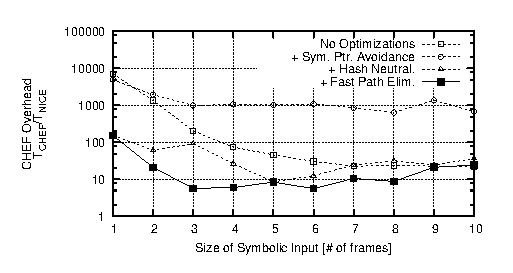
\includegraphics[width=3.2in]{evaluation/graphs/chef/nice-optimizations}
  \caption{Average overhead of \chef compared to \nicese, computed as ratio of average per-path execution times.  The average divides total tool execution time by number of high-level paths generated.}
  \label{fig:nice-overhead}
\end{figure}

Given the small size of the controller (less than 100~LOC), the number of execution paths is relatively small, and choosing low-level paths at random quickly discovers new high-level paths.  Therefore, the search strategy has no impact (in the experiments we used path-optimized CUPA).  However, the interpreter optimizations are crucial, since the controller code relies heavily on the dictionary.  As in Section~\ref{sec:sub:optimizations}, we use several interpreter builds with optimizations introduced one-by-one.

Figure~\ref{fig:nice-overhead} illustrates the overhead for each optimization configuration, as a function of number of Ethernet frames supplied.  The overhead is computed as the ratio between the average execution times per high-level path of \nicese and \chef.  In turn, the execution time per high-level path is computed by dividing the entire execution time of each tool by the number of paths it produced.

%% Basically the same reasons we already gave earlier in the paper

The performance of each optimization configuration illustrates the sources of path explosion and slowdown in the vanilla interpreter.  With no optimizations, symbolic keys in the MAC dictionary cause massive path explosion due to symbolic pointers.  When avoiding symbolic pointers, performance drops even more due to symbolic hash computations.  This penalty is reduced up to two orders of magnitude with hash neutralization.  Finally, fast path elimination reduces the forking inside string key comparisons in the dictionary.

The shape of the final performance curve (the solid line) is convex.  For 1 and 2 symbolic frames, the search space is quickly exhausted and the execution time is dominated by \chef's initialization costs, i.e., setting up the symbolic VM and executing the interpreter initialization inside the guest.  This results in an execution overhead as high as $120 \times$.  For more symbolic frames, the initialization cost is amortized, and the overhead goes below $5 \times$.  However, as the number of frames increases, so does the length of the execution paths and the size of the path constraints, which deepens the gap between \chef's low-level reasoning and \nicese's higher level abstractions.  For 10 symbolic frames, the overhead is around $40 \times$.

Despite \chef's performance penalty, the alternative of writing an engine by hand is daunting. It involves developing explicit models that, for a language like Python, are expensive, error-prone, and require continuous adjustments as the language evolves.
%
Where performance is crucial, a hand-written engine is superior; however, we believe that \chef is a good match in many cases.

%%% Local Variables: 
%%% mode: latex
%%% eval: (visual-line-mode)
%%% fill-column: 1000000
%%% TeX-master: "main"
%%% End:


\chapter{Conclusion}
\label{ch:conclusion}

This thesis addressed two instances of the environment problem, which collectively cover a wide range of real-world software: (1) system software interacting with the operating system, and (2) high-level programs written in dynamic languages, such as Python, Ruby, or JavaScript.  The two instances exhibit opposite characteristics: while the operating system interfaces are typically stable and well-documented (e.g., POSIX), the specifications of dynamic languages are incomplete and unstable.

To address the environment problem for stable operating system interfaces, this thesis introduced \emph{\cnine}, a symbolic execution platform that provides an accurate and efficient model of the POSIX interface, as used by systems such as system utilities, web servers, or distributed systems.
%
\cnine relies on the insight that, for the purpose of testing, the operating system interface can be modeled as guest code on top of a set of basic abstractions: threads and processes, synchronization, and address spaces with shared memory. These abstractions need to be provided as primitives by the symbolic execution engine, while the rest of the model can be emulated as guest code.

For incomplete and unstable dynamic language semantics, this thesis introduced \emph{\chef}, a platform for obtaining symbolic execution engines for interpreted languages by reusing their interpreters as executable specifications.  In \chef, the target program is bundled with the interpreter, running in a low-level (e.g., x86) symbolic execution engine, such that the aggregate system acts as a high-level execution engine for the program.
%
%% Chef automatically maps the low-level interpreter paths to high-level program paths by segmenting each low-level path into distinct high-level instructions.
%
To circumvent the complexity of symbolically executing the entire interpreter, this thesis introduced Class-uniform Path Analysis (CUPA), a heuristic for prioritizing paths that works by grouping paths into equivalence classes according to a coverage goal.

\bibliographystyle{plain}
\bibliography{header-standard,biblio}

\end{document}


%%% Local Variables: 
%%% mode: latex
%%% eval: (visual-line-mode)
%%% fill-column: 1000000
%%% TeX-master: "main"
%%% End:
